 %% Il y a deux façons d'utiliser ce prototype de thèse:
%%       soit vous pouvez pas blairer LaTeX,
%%       soit vous en êtes un gourou.
%% Dans le premier cas, il vous suffira de remplacer ce qu'il faut
%% dans ce fichier pour obtenir presque automatiquement un manuscript qui
%% ressemble à une thèse réglementaire.
%%
%% Dans le second cas, vous ne pourrez vous empêcher d'aller trafiquer
%% le fichier these.sty pour rendre les choses encore plus automatiques
%% (il y a sûrement un moyen de rendre plus élégante la mise en place
%% du résumé sur la quatrième de couverture, par exemple)
%% et l'adapter aux derniers caprices de la Scolarité.
%% SVP, dans ce cas, faites profiter tout le monde de vos améliorations
%% en renvoyant these.sty et un exemple de these.tex au ouaibemestre de l'ADOC.
%%

\documentclass[11pt]{book}
%% En 12pt c'est possible aussi

%% packages utilises
%%---------------------
\usepackage{emptypage}
\usepackage[utf8]{inputenc}
% \usepackage[T1]{fontenc}
\usepackage[frenchb,english]{babel}
\usepackage{amsmath,amssymb}
\usepackage[T1]{fontenc}
\usepackage[usenames,dvipsnames]{xcolor}
\usepackage{amssymb}
\usepackage{these}
\usepackage{array}
\usepackage{floatflt,amssymb}
%\usepackage[draft=true]{graphicx}
\usepackage{graphicx}
\usepackage{moreverb} %% pour le verbatim en boite
%\usepackage{slashbox} %% pour couper les colonnes des tableaux en diagonale
%\usepackage{showkeys} %% pour voir les labels
\usepackage{multirow} %% pour regrouper un texte sur plusieurs lignes dans une table
\usepackage{url} %% pour citer les url par \url
\usepackage[all]{xy} %% pour la barre au dessus des symboles
\usepackage{shorttoc} %% pour plusieurs tables des matières par la commande \shorttableofcontents{Titre}{profondeur}.
\usepackage{textcomp} %% pour le symbol pour mille par \textperthousand.
\usepackage{hyperref} %% pour la transformation en PDF, ça permet d'obtenir des liens sur les sections ...
\usepackage[babel=true]{csquotes}
\usepackage[right]{eurosym}
%\usepackage{algorithm}
%\usepackage{algorithmic}
%\usepackage{algorithm2e}

\usepackage{color}
\definecolor{red}{rgb}{1,0,0}
\definecolor{green}{rgb}{0,1,0}
\definecolor{blue}{rgb}{0,0,1}
\definecolor{cyan}{rgb}{0.4,1,1}
\definecolor{orange}{rgb}{1,0.7,0}
\definecolor{dkgreen}{rgb}{0,0.6,0}
\definecolor{gray}{rgb}{0.5,0.5,0.5}
\definecolor{purple}{rgb}{0.58,0,0.82}
\definecolor{dkgray}{rgb}{0.3,0.3,0.3}

\usepackage{lscape}
%\usepackage{subfigure}
\usepackage{listings}
\usepackage{alltt}

\usepackage{tikz}
\usepackage{pgfplots}
\usepackage{pgfplotstable}
\usetikzlibrary{arrows,shadows,patterns, external}

\tikzexternalize[prefix=auto-figures/]

\usepackage[caption=false]{subfig}

\usepackage{dblfloatfix}

%\usepackage{todonotes}

\usepackage{amssymb}% http://ctan.org/pkg/amssymb
\usepackage{pifont}% http://ctan.org/pkg/pifont
\newcommand{\cmark}{\ding{51}}%
\newcommand{\xmark}{\ding{55}}%
\newcommand{\todo}[1]{{{\em TODO}: \bf #1}}
\newenvironment{mylisting}
{\begin{list}{}{\setlength{\leftmargin}{2em}}\item\scriptsize\bfseries}
{\end{list}}
\newenvironment{mytinylisting}
{\begin{list}{}{\setlength{\leftmargin}{1em}}\item\tiny\bfseries}
{\end{list}}


%
% Command intended to create cool phrases in the beginning of each chapter
%
\newcommand{\coolphrase}[2]{
\noindent\makebox[\linewidth]{\rule{\textwidth}{3pt}}

\begin{verse}
#1
\end{verse}

{\raggedleft{}\textit{- #2}}

\noindent\makebox[\linewidth]{\rule{\textwidth}{1pt}}

%\centering
\vspace{0.5cm}
}



%% macro/racourcis por les symboles et commandes usuelles
\input{./macro}

%% choix des profondeurs de section pour la table des matières
%% 2= subsection, 3=subsubsection
\setcounter{secnumdepth}{3}  %% Avec un numero.
\setcounter{tocdepth}{2}     %% Visibles dans la table des matieres



\makeindex %% crée l'index
\def\underscore{\char`\_}

%% c'est parti mon kiki !!
%%%%%%%%%%%%%%%%%%%%%%%%%%%%%%%%%%%%%%%%%%%
\begin{document}%%%%%%%%%%%%%%%%%%%%%%%%%%%
%%%%%%%%%%%%%%%%%%%%%%%%%%%%%%%%%%%%%%%%%%%

%\hyphenation{im-pl\'e-men-ta-tion}
%\hyphenation{con-train-tes}
%\verb|\checkmark|: \checkmark \par
%\verb|\cmark|: \cmark \par
%\verb|\xmark|: \xmark



\addtocounter{page}{-1}%ça c'est pour revenir à 0
%\fontfamilly{phv}

%%  1ere de Couverture:
\titre{
\begin{flushleft}
Supporting \\ resource-awareness in \\ managed runtime environments.
\end{flushleft}}
%Approche à contraintes pour \\la sélection de \textit{Covering Array}.
%\titre{Sélection de Coverring Array à l'aide des contraintes pl}


%\soutenue
%%   Laisser cette ligne en commentaire sauf pour la version finale.
%%   (la premiere page contiendra "a soutenir le ..."
%%   au lieu de "soutenue le ...")


%% Les différents champs de la couverture...
\datesout{18 November 2015}
\Auteur{Inti}{Gonzalez-Herrera}

\Labo{INRIA}
\LaboEtendu{Rennes Bretagne Atlantique} % sauf INSA
\ComposanteUniversitaire{} % sauf INSA

%% La composition du jury : prénom, nom, titre
%\President[M]{Thierry}{Jeron}{Directeur de recherche à l'INRIA}         %% le président du jury
\Advisor{Benoit}{Baudry}{Chercheur, INRIA Rennes - Bretagne Atlantique}
\Advisor{Johann}{Bourcier}{Maître de conférences, Université du Rennes 1}
\Advisor{Olivier}{Barais}{Maître de conférences, Université du Rennes 1}
\Rapporteur{John}{Doe}{Place 1}
\Rapporteur{John}{Doe}{Place 1}
%% Si vous avez N rapporteurs ça marche toujours...
\Examinateur[Mme]{John}{Doe}{Place 1}
\Examinateur[M]{John}{Doe}{Place 1}
%% idem...

%\ordre{00000}  %% le numéro d'ordre donné par la Sco
\makethese{rennes1}    %% crée la couverture.


%% une page blanche (deuxième de couverture)

\newpage\thispagestyle{empty}\addtocounter{page}{-1}
~\newpage\thispagestyle{empty}\addtocounter{page}{-1}

%%  une page de citation (pas indispensable)


%% Encore une page blanche pour que les remerciements arrivent
%%  sur une page impaire

\newpage\thispagestyle{empty}\addtocounter{page}{-1}
~\newpage\thispagestyle{empty}\addtocounter{page}{-1}

%\remerciements
%\remerciements{Il faut vraiment que je dise merci ? :o)}
%% vous n'êtes pas obligés d'utiliser cette commande
%% mais elle vous donnera une idée de la chose

\newpage\thispagestyle{empty}\addtocounter{page}{-1}

%% pour cacher le numéro de page sur cette page blanche paire
%% (à virer si vous avez plus d'une page de remerciements.)

%%----------------------------%%
%%                            %%
%%  TABLE DES MATIERES        %%
%%                            %%
%%----------------------------%%

%\newpage\thispagestyle{empty}

%~\newpage
\addcontentsline{toc}{chapter}{Table of content}
\markboth{Table of content}{Table of content}
\tableofcontents%%{Table des matières}

%%----------------------------%%
%%                            %%
%%  CHAPITRES PRINCIPAUX      %%
%%                            %%
%%----------------------------%%

%------------------------------%
%------------------------------%


\chapter{Introduction}
%\addcontentsline{toc}{chapter}{Introduction}
%------------------------------%
%------------------------------%
\markboth{Introduction}{Introduction}

\coolphrase{
This is the text
}{inti}

\section{Motivations and Overview}

Software systems are becoming even more pervasive nowadays.
From simple applications for controlling home appliances to complex tools for dealing with productive processes, software systems are now found in any environment.
The end-user's expectations have also grown along the development of the software industry.
For instance, installing several applications provided by non-fully trusted sources in a mobile phone or closing a window in your office through a website are considered nowadays routinary  tasks which only require engineering effort.
However, the software/hardware industry faces several problems while coping with these expectations.
Among these challenges we find the need to handle millions of users, the ubiquity of resource-constrained devices, and the
open nature of execution environments.   

The widespread usage of interconnected devices and the trend to use client/server architectures have led to a massive increment in the number of users some applications have to deal with.
To support so many users, it is necessary to manage a massive computing infrastructure which is both complex and extremely costly.
The emergence of cloud services was a \textit{natural} development of these infrastructures.
Cloud services, which often are used to  build client/server applications,  are all about providing access to computing resources.
They are shipped in many forms (e.g., virtual machines, software) but in general we can reduce them, using a rather simplistic model, to basic resources such as CPU cycles, memory, network bandwidth and storage capacity.
This simplistic view is useful if we consider how important is for cloud services providers to reduce the usage of resources in order to increase efficiency.
For instance, given the large nature of the cloud, a provider of platform as a service (PaaS) can reduce the operational costs if it manages to squeeze even a few thousand of bytes from each request.
As a consequence, carefully managing resources such as CPU and memory becomes a primary concern for cloud service providers.

Despite of the continuous evolution of hardware, demand of applications often surpasses hardware capabilities.
This limitation of resources is particularly clear in wearable devices, but in the near future we can expect to see the same kind of concern in the emergent \textit{Internet of Things}.
In this kind of devices it is fundamental to offer tools for properly sharing the scarce resources among applications.
It is worth noting that managing resources has been a central problem in computer science and software engineer for a long time.
However, I highlight the problem in this context for two reasons.
First, because I think that new technologies to build applications for these devices allow better resource management techniques.
Second, because it shows that limitations in resource quantity is still a concern for software developers.

Open execution environments refer to the possibility of allowing the deployment of applications provided by different sources at any time, being these sources trustworthy or not.
Since end-users are able to install many applications that share the execution environment, it is impossible for the developers of the runtime or of a single application to predict under what condition an application will be executing.
Guarantying isolation among applications is of utmost importance because now it is possible to use these execution environments to build and massively deploy actuators that operate on the physical environment.
A possible source of failure in these applications is the lack of resource isolation.
In short, an application makes another to fail by consuming the resources needed for the later.

The common concern in the three previous problems is that of making applications and execution environments aware of and capable of coping with resource limitations. 
To the problem of 
This thesis addresses the problem of supporting resource-aware programming in execution environments.
Given their popularity, it focuses on facing the issue of resource-awareness in managed runtime environments (MREs) such as Java and the CLR.

Existent solutions for resource management in MREs have two fundamental problems.
First, they impose a significant performance overhead while monitoring the resource consumption of applications.
Second, despite of the broad usage of MREs to execute component-based applications and to build domain-specific 
abstractions, it is still had to provide tools to seamless deal with the resource management concern.

\if 0 


\subsection{General Objective}
Offering portable support for \textbf{resource-aware programming} in \textbf{managed runtime environments}.

Disminuir el costo de gestionar recursos en tiempo de ejecucion y facilitar el uso de tecnicas de resource-aware programming en ambientes de ejecucion manajeados.

Ofrecer soporte para la resource-aware programacion en ambientes de ejecucion manejados. 
\todo{Soporte es un termino ambiguo, lo de portable tambien es dificil de enteder en el contexto}

\subsection{Specific Objectives}
\begin{enumerate}
\item Reduce the amount of CPU and memory used to determine the resources consumed by different parts of an application built to execute on top of managed runtime environments.\\
Reducir la cantidad de CPU y memoria utilizada para determinar los recursos consumidos por diferentes partes de una applicacion construida para ejecutarse 
sobre un ambiente de ejecucion manejado.\\

\item Provide abstractions for supporting the development of tools to efficiently measure at runtime the memory consumed by domain-specific abstractions that were implemented atop the \textit{classic} object-oriented paradigm.

Proveer abstracciones que permitan crear
herramientas eficientes para medir en tiempo de ejecucion la memoria consumida por abstracciones de dominio especifico que fueron implementadas usando el clasico paradigma orientado a objetos.\\

\todo{Preguntar las 4 preguntas y si el como va en el objetivo especifico. Mami como yo conformo un objetivo.. el problema que yo veo aqui es que no es facil medir lo e aligerar el desarrollo. Necesito estudio con usuarios  eso no lo hice.}
\item Reduce the complexity and computational cost of managing resource reservation in component-based software systems.

Reducir la complejidad y costo computacional de gestionar la reserva de recursos en sistemas basados en componentes.
\end{enumerate}

\subsection{Research questions}

\subsection{Research justification}

\subsection{Viabilidad de la investigacion}

\subsection{Contributions}
\begin{enumerate}
\item A methodology for resource-management-aware component deployment.
\item An optimistic resource monitoring approach that reduces the performance overhead.
\item A domain-specific language to developed custom memory profilers.
\end{enumerate}

En la introduccion, ademas de declarar cuales son los objetivos de la tesis y las contribuciones de la misma, debo hacer una breve recapitulacion de los elementos fundamentales a tratar. La estructura es por supuesto la tradiccional de contexto, problema, solucion propuesta y como la evaluamos. Sin embargo, es quizas aportuno agregar algo como impacto esperado de esta investigacion. 

\fi

\section{Dissertation Structure}
%\part{Background and State of the Art}
%------------------------------%
\selectlanguage{english}
\chapter{Background on resource awareness}
\label{chp:background_resource_awareness}
\markboth{Background on resource awareness}{Chapter1}
%------------------------------%

\coolphrase {Hey, look at this}{Inti Gonzalez-Herrera}

\section{Resource Awareness}

\section{System support for resource awareness}

\begin{itemize}
\item CGroup
\item FreeBSD
\item \dots
\end{itemize}

\begin{comment}

\begin{itemize}
\item Resource-aware programming, a broad view. \\
The \textbf{goal} of this section is to introduce and discuss the main concepts regarding resource-aware programming.
In short, I am going to present how important is, in some contexts, developing applications which are able to monitor and manage the resources consumed.
This is specially important in middleware, system with continuous evolution and open environments.
I shall mention the goals we pursuit when we put attention to the resource consumption's concern: QoS, reliability, availability, performance, security, resource-constrained devices.
This section also mentions how this important not only for applications but for applications framework too.

\textbf{Discuss} the following topics that are related to resource management:
\begin{itemize}
\item Resource monitoring
\item Resource reservation
\item Resource isolation
\item Reflection
\end{itemize}

\item Resource monitoring and reservation technologies.\\
Aqui \textbf{discutire} los metodos para hacer monitroing and reservation. Primero algo muy general, pasando a discutir el tema y su importancia in nowadays managed runtime enviroments. La mayoria de este contenido puedo tomarlo desde el reporte.

Los \textbf{objetivos} son: destacar las tecnologias que hay, mencionar sus limitacion. Las limitacion a destacar son: el problema de la portabilidad (muchas implementaciones de la JVM), el problema del performance, el problema de lidear con variadas abstracciones de dominio especifico. 

\item Domain-specific abstractions. \\
En esta seccion se discutira escencialmente que son los domain-specific languages y caules son sus limitaciones en relacion a tooling support cuando se trata de profilers y debuggers. Argumentar esta carencia es facil cuando hablamos de lenguages como Xtend y Kermeta3. Para lenguajes mas especificos como el ubiquo State Machine ya no es tan facil de argumentar porque esas abstracciones no tienen un modelo de ejecucion tan claro o si lo tienen entonces el consumo de memoria no es relevante.

\item Component-based software engineering.\\
Esta seccion \textbf{discute} primero, y solo brevemente, los elementos fundamentales de CBSE, sus ventajas y nivel de adopcion en la practica. Por ultimo menciona que existen varios modelos de componentes y hace una breve recapitulacion de los mismo haciendo enfazis en aquellos que tienen implementacion en managed runtime environments.
Es vital en esta parte hacer una descripcion de los aspectos de estos modelos que los hacen unicos o similares en terminos de control de recursos.
Lo siguiente es relacionar componentes con resource-aware programming. In short, como los modelos de componentes pueden beneficiarse de resource-aware programming para ofrecer un ambiente mas util a los componentes. 

Disutir como el concepto de componente es un tipo especial de abstraccion que presenta para un monitor de consumo de memoria los mismos retos que otras abstracciones. Por lo tanto, debe de intentar generalizarse la definiciones de monitores de consumo de memoria

Me pregunto si debo usar aqui el termino middleware?

Los \textbf{objetivos} de la seccion son: enmarcar la tesis en un contexto de componentes, resaltar la utilidad y desafios de hacer resource-aware programming for component models. Ademas, DEBE decirse what have been done en resource-aware programming y resource mangement para modelos de componentes en el pasado.
Entonces viene la parte dificil: indicar las limitaciones de lo existentes. En mi opinion, no son tanto limitaciones como enfoques diferentes, o quizas la limitacion esta en que el proceso de seleccion del component binding nunca ha estado dirigido por la necesidad de disminuir el overhead de hacer resource management at runtime.

\end{itemize}

\end{comment}
%\part{Contributions}
\selectlanguage{english}
\chapter{Squirrel: Architecture Driven Resource Management}
\label{chp:squirrel}
\markboth{Squirrel: Architecture Driven Resource Management}{Chapter5}

\coolphrase {
	I still don't know
}{Some name here}


%Resource management is critical to guarantee Quality of Service when various stakeholders share the execution environment, such as cloud or mobile environments.
%In this context, providing management techniques compatible with standard practices, such as component models, is essential.
%Resource management is often realized through monitoring techniques, while resource isolation uses virtual machines or containers (e.g., docker).
%These techniques (i) impose varying levels of overhead depending on the managed resource, and (ii) are applied at different abstraction levels, such as processes, threads or objects.
%Thus, mapping components to system-level abstractions in the presence of resource management requirements can lead to sub-optimal systems.
%
%We propose Squirrel, an approach to tune component deployment and resource management in order to reduce management overhead.
%At runtime, Squirrel uses an architectural model annotated with resource requirements to guide the mapping of components to system abstractions, providing different resource management capabilities and overhead.
%We present an implementation of Squirrel, using a Java component framework,
%and a set of experiments to validate its feasibility and overhead.
%We show that choosing the right \textit{component-to-system} mappings at deployment-time reduces performance overhead and/or memory use.

\section{Introduction}

Resource management is critical for domains where software components share an execution environment but belong to different stakeholders.
For instance, in multi-tenant systems resource management is used to guarantee safety, reliability and per-stakeholder Quality of Service (QoS).
These applications essentially require the isolation of tenants in terms of resource consumption~\cite{KrWeKo2013-icwe-MTBenchmark}.
This enables, for example, \textit{Software-as-a-Service} layers for cloud systems, allowing innovative pricing policies based on user requirements. %(e.g. user A has a \textit{premium} contract that guarantees a response time inferior to 500 ms for each request, while user B has a \textit{standard} contract that does not guarantee any response time).
Since these services are often implemented on paradigms such as component models,
the design of resource management techniques dedicated to component models is an important issue.

Component model implementations represent high level concepts, such as component instances, by means of mapping them to system-level abstractions like objects, threads, processes or virtual machines.
Each mapping has unique features in terms of performance, memory footprint, etc.
However, these mappings are often done in a once-size-fits-all manner, allowing some choices to optimize for memory use while others might, for example, improve inter-component communication.
%\hl{The mapping of components to system abstractions, which has the goal of improving some parameters of the runtime, has often been made in a homogeneous way for all components.[I DON'T UNDERSTAND?, Quiero decir que todos los componentes usan el mismo mapping, todos son representados como hilos, o todos como procesos. La parte de ``som parameters'' significa que cuanod se toma esa decision durante la implementacion del framework se hace con un objetivo como reducir el uso de memoria o facilitar la comunicacion entre componentes o garantizar un ``sandbox'' para los componentes]}
Interestingly, system abstractions offer varying resource management capabilities that differ in how they impact the application.
Although we can hard-code the resource management concern during the design of the component model, we argue that this leads to sub-optimal systems with high  overhead~\cite{binder_portable_2006,czajkowski_jres:_1998,Maurel:2012:AME:2304736.2304763} because components have different resource requirements.

% without taking into account resource management concerns, and (ii) .

To address this issue, we propose Squirrel, an approach to resource management for component models that aims at reducing overhead.
In Squirrel, the application is deployed with a model containing resource usage contracts for each component and a detailed view of the system.
These metadata are used to choose at deployment-time the best way of representing each component in terms of system abstractions.
This contrasts with the \textit{traditional} approach of binding the representation during the design of the component model and results in the final runtime representation of the system only being known after deployment.
%uses meta-data regarding the application's structure and its requirements to deploy components on system-level abstractions.



%During deployment, the information is used to automatically create a new deployment model where components are automatically mapped into abstractions that we call \textit{containers}.
%Each \textit{container} is then configured based on the components' resource contracts, ensuring resource consumption while minimizing the overhead.

In this paper we discuss an approach to resource management applicable to any component model. To validate the feasibility of our proposal, we present a reference implementation for a Java-based component model.
A set of experiments validate its feasibility and show various aspects of its overhead.
The results demonstrate that choosing the right \textit{component-to-system} mappings at deployment-time can reduce performance overhead and/or memory footprint.
%\hl{INTI: Se que esta oracion es muy general, el problema es que no estoy seguro de si poner los numeros es lo correcto pues los ejemplos son tan solo para mostrar con un caso de uso los potenciales beneficios de postergar la decision acerca de como hacer el manejo de recursos.}
The contributions of this paper are as follow:
\begin{itemize}
\item An approach for architecture driven resource management that leverages structural information to guide the mapping of component model concepts onto system-level abstractions.
\item A reference implementation of the Squirrel framework for a Java-Based component platform.
\item A performance comparison showing how different mappings can impact the overhead of the system and how the approach behaves in comparison to state-of-practice approaches for resource management.
\end{itemize}

The remainder of this paper is organized as follows.
The next section presents some foundational work we use along this paper.
Section \ref{sec:apprach} describes the Squirrel approach and presents how we leverage metadata to drive resource management.
In section~\ref{sec:kevoree} we propose a reference implementation of Squirrel for a Java-based component platform.
A validation of the implementation through a set of experiments is presented in section~\ref{sec:evaluation}.
Finally, section \ref{sec:related-works} discusses related work and section \ref{sec:conclusions} presents our conclusions and future work.


%\section{Background on resource management }

%\textbf{Synthesis.}
%Providing resource management features at the application level is possible, but it introduces high overhead in the application \cite{gonzalezherrera:hal-00983045}, thus greatly limiting its interest.
Current middleware either provide limited resource-awareness or totally hide resource concerns from the application.  Following the same ideas as in \cite{guerraoui1999oo} where authors explain that the distribution concern should not be hidden from developers in object-oriented distributed programming, we believe that the resource management concern should not be hidden from application developers. We envision combining monitoring techniques and system-layer resource management techniques to achieve this goal. 
This section presents a summary of two underlying techniques used to monitor and reserve resources. 



%These approaches are used in section~\ref{sec:kevoree}.

%Providing adequate support for pervasive applications is a challenge because their resource requirements vary (e.g., processors, memory bandwidth, I/O).
%For critical applications, such as surveillance systems, a known bounded amount of resources must be guaranteed for the application to run properly. For multimedia applications, the amount of required resources may change over time and dynamic adaptations and redeployment can be required. 

%Lots of modern middleware are typically implemented using Java (for example with OSGi) because of its safety, flexibility, and mature development environment.
%However, the Java virtual machine was designed to execute a single application at a time and does not provide \textit{per-component} resource reservation.
%Current Java-based middleware are thus unable to reserve resources for critical applications, which may cause these applications to crash or hang when insufficient resources are available.

%As an example, we can consider a smart home system that simultaneously provides services that are critical for user safety, and services that increase user comfort. 
%For example, a smart home system can provide a health monitoring service for elderly people allowing them to stay at home while regularly reporting on their health and quickly raising alarms in case of emergency. 
%The same system can simultaneously provide services for closing all shutters at night or to access multimedia content.
%All these services constantly evolve after their initial deployment and thus their behavior and requirements regarding resource consumption may change accordingly.
%For these environments, where services featuring various degrees of criticality share the same execution environments and thus the same resources, a mechanism to guarantee resource access and priority is required.

\textbf{Cgroups} (control groups) is a Linux kernel feature to limit, account, and isolate the resource usage of processes. 
It provides a low-level API to access properties on resource usage that allow to i) limit memory consumption per task, 
ii) assign a minimum percentage of CPU time to the task,
iii) establish a minimum and maximum throughput for I/O block devices and network throughput per task, and
iv) measure the resources a task uses.
Cgroups are used in particular in the context of lightweight process virtualization (e.g., OpenVZ, LXC).


\textbf{Scapegoat} provides an application-level adaptive resource monitoring framework~\cite{gonzalezherrera:hal-00983045}.
Each component is augmented with a contract that specifies its resource usage, such as peak CPU and memory consumption.
The framework adjusts the monitoring level to minimize overhead while still allowing precise accounting when needed.
The adjustment is done by selecting, through a heuristic, components that should be deeply monitored using intrusive instrumentation to check their contracts, while using a lightweight monitoring mode the rest of the time.
%Furthermore, Scapegoat proposed a heuristic that leverages information produced by the Models@runtime approach to quickly predict the faulty components.


%They are considered one of the building blocks to support Linux containers.



\section{Approach} \label{sec:apprach}

The main concept in Squirrel is the \textit{resource-aware container}.
Such containers are logical entities that take care of the resource management concern.
By logical we mean that it is not important, from a functional point of view, how a
container achieves resource management. 
Instead, a resource-aware container is an entity that \textit{wraps} a set of components and offers the following properties:
\begin{itemize}
\item \textbf{Resource consumption monitoring} refers to the ability to assess the 
quantity of resources used by a component.
\item \textbf{Resource reservation} is the capacity to ensure a given amount of
resources will be available whenever a component demands it.
\item \textbf{Resource isolation} guarantees that a component's behavior in terms
of resource usage does not interfere with the behavior of another component.
\end{itemize} 

%Even the idea of 
\textit{Wrapping} a set of components can be considered a soft definition because the \textit{membrane} of a resource-aware container limits the behavior
of the contained components only when it is relevant to the resource management concern.
For instance, components within different containers can still communicate directly
with each other through their interfaces without intervention of their containers as long as such communication does not affect the resource under management.  

In Squirrel we propose to automatically select, deploy and configure resource containers to manage resource usage.
The novelty is that we delay the selection of the container's implementation till deployment-time in order to have knowledge about the exact conditions of the system and thus minimize the overhead of the resource management system.
This idea is supported by the claim that components often require disjoint sets of resource types.
Our framework is composed of three essential elements: i) a mechanism to describe the management requirements of an application, ii) an admission control scheme in the middleware to handle the global view of resource availability, and iii) mechanisms to map component model concepts to system-level abstractions.
In the following subsections we describe our framework and its elements.

\subsection{Managing resources through architecture adaptations}
Modern application development models, such as component-based systems, promote the usage of Architecture Description Languages (ADL) or configuration models to check properties on the system's structure and to drive system deployment. 
In Squirrel, we propose to enhance this layer with metadata regarding resource reservation and to use these metadata to efficiently drive resource reservation offered at the system level.  
The idea is to follow a gray-box approach where we automatically adapt a component-based application by applying an architecture pattern to isolate a component within a resource-aware container.

\begin{figure}[htbp]
\centering
\includegraphics[width=0.7\textwidth]{chapter4/figures/globalOverview.png}
\caption{Squirrel approach for resources reservation} \label{fig:Overview}
\vspace{-0.5cm}
\end{figure}	

As illustrated in figure~\ref{fig:Overview}, Squirrel follows an automatic process to manage resources.
Squirrel receives an application's model, enhanced with contracts on resource reservation. 
Squirrel performs admission control to check the validity of the contracts on resource usage with respect to the available resources in the execution environment.
If the contracts are consistent with available resources, the process continues, if not, the application's model is refused.
Then, as depicted by arrow 2, Squirrel automatically transforms components or the configuration/architecture model by isolating components in resource-aware containers that can be finely configured to decrease the resource management overhead.
Finally, as depicted by arrow 3, Squirrel reconfigures the running system.
When the application evolves (arrow 4), 
%Squirrel automatically adapts the system while preserving resource reservation properties by applying the whole process on the new model (arrow 5, 6 and 7).
Squirrel attempts to preserve resource reservation properties while processing the new model (arrow 5, 6 and 7).


\subsection{Describing resource management requirements}
Beugnard et al. discuss the extending Meyer's \textit{Design-By-Contract} idea to software components~\cite{Beugnard774917}.
They classify component contracts into four categories: syntactic (level 1), semantic (level 2), synchronization (level 3), and Quality of Service (level 4).
%They explain that component contracts have to deal with concerns that they classified into 
%Fifteen years later, many component-based frameworks provide contracts that are used to: 
%i) Describe the component features with all required contracts.
%ii) Select from all contracts those that are useful in the context of component use, and configure them.
%iii) Evaluate contracts and react accordingly.
%iv) Decide when to stop evaluating contracts. 
There is no de-facto standard to describe component contracts, but many domain specific interface description languages contain such metadata.
This chapter assumes that components have contracts to deal with resource reservation (level 4).
A contract in Squirrel defines component resource requirements written in terms of resource types, quotas and expected component usage.
\begin{itemize}
\item{\textbf{Definition 1}} A resource type indicates any class of computational resource that is useful to a component.
Its consumption must be susceptible to monitoring and reservation.
In this paper, we consider CPU, Memory, Network Bandwidth and IO Throughput.

\item{\textbf{Definition 2}} Expected component usage describes the expected number of external invocations of each method of the component interface.
In short, let $C$ be a component instance, then $\forall{I \in C_{Interfaces}}, \forall{M \in I_{methods}} \\ {EU}_{IM}$ is the number of expected invocations of method $M$, per second.

\end{itemize}

A \textbf{contract in Squirrel} is a set of tuples with the form $\langle RT, N, MU \rangle$ where $RT$ is a resource type, N the maximum amount of resources to reserve, and $MU$ is the measuring unit used for this resource type.
Optionally, Squirrel supports the definition of a set of tuples with the form $\langle I, M, {EU}_{IM} \rangle$ where $I$ is a component interface, $M$ is a method of the interface, and ${EU}_{IM}$ the expected usage.
Implementations of the Squirrel approach must provide a way to define contracts with these concepts.
%In section~\ref{sec:kevoree} 
We use a domain-specific language to describe contracts.

\subsection{Admission control} \label{sect:admissionControl}

Providing resource reservation in a component based framework requires checking if components' resource-aware contracts are compatible with the resources available in the execution environment.
%The platform provides a fixed amount of resources that constitute the pool of resources used by components.
By checking the availability of resources, the platform controls component admissions.

%To support this dynamism while managing resources, 
To support resource management at runtime, Squirrel takes into account two events: i) component deployment, and ii) component removal.
%These are common operations on any middleware; hence adding a notification for these events is straightforward.
Whenever the application is modified, the system automatically recalculates the aggregated resources required by the application and compares it to the available resources in the execution environment.
If the available resources are greater than those required by the application, the reconfiguration is accepted, else, the application model is refused and the reconfigurations are discarded.

%\subsection{Defining multiple variants of execution model}
%\todo{I couldn't finish this, so I'm writing my ideas}
%To support our approach, a middleware needs to support multiple ways of mapping component instances into system/runtime abstractions.
%Somehow, it means that it needs an extension point to describe a factory for creating component instances.
%I can see two ways of doing so, either the writer of the middleware provides many versions of execution model or she provides a mechanism to extends the semantic of a component instance and of component containers (Node).
%In Kevoree we achieved this easily because it is naturally extensible, we can define new Node Types, New Channel Type, and we can compose them.
%Moreover, we use Models@Runtime to easily change between variant of mappings (e.g., we receive a model where each component is executed as a Thread and sometime we transform the model in order to execute components as processes). 

\subsection{Mapping component-model concepts to system-level abstractions}

%To map component-model concepts to system-level abstractions that allow for resource management, Squirrel defines steps to perform either during the design/implementation of the platform or at deployment time.
Squirrel defines steps to map component-model concepts to system-level abstractions that allow for resource management. Mappings can be applied during the design and implementation of the framework, or at deployment-time.
During framework design/implementation, developers identify system abstractions that are suitable to represent each concept and implement the respective mappings.
As a second step, resource management methods for each abstraction are implemented and evaluated.
This evaluation is used to determine the management methods with lowest overhead for each pair of system abstraction and resource type.
Later on, at deployment-time, the platform selects a component-to-system mapping using optimization techniques and the data obtained at design-time.
In this section, we briefly explain each step.

As we have mentioned, components can be represented through different system abstractions. % in the runtime platform.
This requires \textit{identifying possible mappings from components to system-level abstractions}.
Mappings must respect the semantics of the component model, and %but for a resource-aware platform, 
must provide resource management capabilities.
A key problem is that different mappings have different non-functional properties, and optimizations are often needed to make the mappings attractive. % competitive.
Additionally, an extensible design of the component platform, where it is easy to accommodate new mappings, greatly facilitates the co-existence of different mappings to represent a component. 
The set $ \textit{SA} $ of system abstractions that are available to represent a concept, along with the recommended optimizations for each abstraction, are defined in this step.

During the design/implementation of the platform it is necessary to \textit{define methods to manage resources} for each pair of system abstraction and resource type.
Developers must devise resource management methods for each mapping
% and resource type, 
 and identify the least costly.
If we consider different abstractions and resource types, we can define the matrices $ M $ and $ C $ where
$ \forall{\textit{sa} \in \textit{SA}, \textit{rt} \in \textit{RT}} $ the values
$  M_{\textit{sa}, \textit{rt}} $ and $ C_{\textit{sa}, \textit{rt}} $ indicate the method that minimizes the cost of managing the resource $ \textit{rt} $ when the abstraction $ \textit{sa} $ is used to represent a component. %, and this minimum cost.
%\hl{In a simple setting, the cost of each pair could be calculated as the mean overhead produced by the management method when some benchmarks are executed.[IS THIS PHRASE NECESSARY?]}
We make two assumptions about the resource management mechanisms: i) mechanisms are always composable if they manage different resource types, and ii) the costs of any pair of management mechanisms are independent.

At deployment-time, \textit{the platform selects the mapping} to use for each component in the application. % to deploy.
To do so, the platform uses the information contained in the matrices $ M $ and $ C $, the set of possible optimizations for each mapping, and the resource requirements of the application.
At this stage, the only data needed regarding resource requirements is the type of resource.
%Using this data, it is possible to apply an optimization method to select the best mapping candidate.
Using this data allows selecting the best mapping candidate.
Although we only use a single cost matrix that contains the overhead of each management mechanism, we think it is easy to generalize the approach to handle multi-objective optimizations with more than one cost matrix.
Others refinement to evaluate the cost of a mapping are possible.
For instance, we can consider the cost of using a specific binding to connect two components that use a given mapping.
Finally, there are many optimization methods that can compute the mappings, we do not propose any particular method in the approach.
However, the results shown in section~\ref{sec:evaluation} suggest that very simple heuristics can lead to good performance. 
 

%\todo{Here we should talk about the heuristic. We are trying to optimize, so we need to choose a mapping for each component. We only have a partial information about each resource managment mechanism. that's why we cannot perform classic optimization and we relies on heuristics}
%\todo{A conclusion here}


\section{Reference Implementation} \label{sec:kevoree}
%\fixme{The beginning of this section needs work, it starts by saying we introduce kevoree, then introduces models@run.time, then kevoree.}

Squirrel's reference implementation exploits the modesl@run.time approach and provides resource-awareness capabilities to the Kevoree component framework~\cite{Fouquet:2012:DCM:2304736.2304759}.
%to support models@run.time.
%We begin with a brief overview of Kevoree.
%Built on top of dynamic component frameworks, models@run.time denotes model-driven approaches to tame the complexity of dynamic adaptation~\cite{Morin:2009:TDA:1555001.1555028}.
Models@run.time denotes model-driven approaches to tame the complexity of dynamic adaptation~\cite{Morin:2009:TDA:1555001.1555028}.
%It pushes the idea of reflection one step further by considering the reflection-layer as a model.
The ``model at runtime'' is a reflection model that can be decoupled from the application (for reasoning, validation, and simulation purposes) and then automatically resynchronized.
Models can manage not only the application's structural information (i.e., the architecture), but can also be populated with other information, such as runtime monitoring data.

Kevoree is a component framework for distributed systems that builds and maintains a structural model of the system, following the models@run.time paradigm.
%and builds a structural model of the distributed system.
Kevoree is mainly used because: (i) it presents a snapshot of the distributed system, and (ii) it provides a language to drive the reconfigurations. 
\textit{Component} and \textit{Channel} are two of the concepts used in Kevoree models.
The former represents software units that provide the business value.
The latter, with the same role as connectors, are in charge of inter-component communication.
Channels encapsulate communication semantics (e.g., synchronous, unicast).

\subsection{A resource-aware container for CPU and I/O reservation} \label{sec:cgroups-based-reservation}

Our implementation leverages resource-reservation mechanisms at the system-level to provide containers for CPU and I/O reservation.
More specifically, it maps the concept of \textit{container} onto a \textit{cgroup}.
Both \textit{containers} and \textit{Kevoree components} are hierarchical structures that are easy to map onto cgroups' hierarchy.
Indeed, a container deploys components and a component runs threads.
To configure the container we setup a hierarchy of cgroups
using the following rules:
\begin{enumerate}
\item
%A fixed amount of resources are reserved for the Kevoree framework, which includes the components of the managed system. This serves as the upper resource-limit.
%To implement this rule we execute the Kevoree framework under a cgroup, while unmanaged applications are expected to run under other cgroups for isolation.
The Kevoree framework is started under a cgroup, using a fixed amount of resources that will be divided among the system's components. 
% that determines the total resource pool. % are reserved (for both).
%This value serves as the pool of resources the framework may use to deploy components.
%On the one hand, it is the maximum amount of resource the container will use when all the threads inside are demanding.
%On the other hand, it is the minimum amount it will receive when other applications outside the container are demanding.


\item
%We create a new resource-aware container for each component, represented by a cgroup.
Each component gets a new resource-aware container, also represented by a cgroup.
The component's contract is translated into a slice $S_c$ of the initial resource allotment, and the result is passed to
%configuration parameters to the cgroup.
the cgroup as configuration parameters.
A slice represents the
%minimum and maximum quantity of 
resources the component has available.
%This means that, although we support resource reservation, we are not supporting overcommitment.
%Since the scheduling unit for cgroups is a thread, we assign threads to cgroups in order to enforce resource reservation.
%However, we cannot assign threads directly to their component's cgroup because then all of them will obtain the same slice $S_c$.
%What we want is to share $S_c$ among all the threads within a component.
%Therefore, a \textit{hidden cgroup} is created that inherits the slice $S_c$ and provides a share to any thread assigned to it by using  \textit{Relative Shares Tunable Parameters}.

\item Since the scheduling unit for cgroups is a thread, we assign the component's threads to the cgroup to enforce resource reservation.

%\item Threads are assigned to the \textit{cgroup} created for the thread owner's component.
\end{enumerate}


\begin{figure}
\centering
%\usetikzlibrary{shadows,arrows}

% Define block styles  
\tikzstyle{cgroup_sty}=[draw, fill=white!20, text width=5em, text centered,
  minimum height=1.4em, rounded corners]

\tikzstyle{thread_sty}=[draw, thin, fill=yellow!20, text width=3em, text centered,
  minimum height=1.4em,dashed]

\tikzstyle{cgroup_container_sty}=[cgroup_sty,fill=gray!20]

\tikzstyle{cgroup_container_hidden_sty}=[cgroup_container_sty,dotted]


\tikzstyle{line} = [draw, thick, color=black!80, -latex']

% commands
\newcommand{\cgroup}[2]{node (p#1) [cgroup_sty]
  {{\scriptsize{#2}}}}

\newcommand{\cgroupContainer}[2]{node (p#1) [cgroup_container_sty]
  {{\scriptsize{#2}}}}

\newcommand{\hiddenCgroup}[2]{node (p#1) [cgroup_container_hidden_sty]
  {{\scriptsize{#2}}}}

\newcommand{\thread}[2]{node (t#1) [thread_sty]
  {{\scriptsize{#2}}}}

\begin{tikzpicture}[scale=0.7,transform shape]
\path \cgroup {1} {Root CGroup};
\path(p1.south) + (-2,-1.2) \cgroupContainer {2} {Cgroup for Kevoree};
\path(p1.south) + (1.7,-1.2) \cgroup {3} {Cgroup for other apps};

\path(p2.south) + (2.3,-1.2) \cgroupContainer {4} {Cgroup for Component2};
\path(p2.south) + (-1.5,-1.6) \cgroupContainer {5} {Cgroup for Component1};

%\path(p4.south) + (0,-1.0) \hiddenCgroup {6} {Hidden Cgroup};
%\path(p5.south) + (0,-1.0) \hiddenCgroup {7} {Hidden Cgroup};

\path [line] (p1) --  node [left] {50\%} (p2);
\path [line] (p1) --  node [right] {50\%} (p3);

\path [line] (p2) --  node [left] {45\%} (p4);
\path [line] (p2) --  node [left] {10\%} (p5);
%\path [line] (p5) --  node [left] {100\%} (p7);
%\path [line] (p4) --  node [right] {100\%} (p6);

\path(p5.south) + (-1.5,-1.2) \thread {1} {Thread1};
\path(p5.south) + (1.8,-1.0) \thread {2} {Thread3};
\path(p5.south) + (0,-1.7) \thread {3} {Thread2};

\path(p4.south) + (0,-1.2) \thread {4} {Thread4};

\path [line] (p5) --  node [above,left] {33\%} (t1);
\path [line] (p5) --  node [above,right] {33\%} (t2);
\path [line] (p5) --  node [left] {33\%} (t3);

\path [line] (p4) --  node [right] {100\%} (t4);

\end{tikzpicture}
\caption{Reserving CPU by mapping components to cgroups} \label{fig:Mapping}
\vspace{-0.5cm}
\end{figure}

This scheme is used for CPU, I/O throughput and network bandwidth.
Each type of resource requires a different \textit{container type}.
% since configuring the container depends on varying properties defined on each cgroup subsystem.
Figure \ref{fig:Mapping} shows an example 
%of how our implementation uses 
using cgroups to reserve CPU for a system with two components.
In the tree, every edge is labeled with the cgroup's CPU slice.
% the cgroup obtains from its parent.
A slice is set for Kevoree, while unmanaged apps are maintained in separate containers.
Applying rule 2, CPU slices are assigned to \textit{Component 1} and \textit{Component 2} according to their resource contracts.
Following rule 3, every thread in \textit{Component1} receives $ 33\% $ of the component's slice.
%When configuring the containers, we apply rule 2 and assign \textit{Component 1} and \textit{Component 2} CPU slices according to their resource contracts.
%Finally, slices for Kevoree and for the rest of the system are assigned.
%In our case, we selected as description the number of instructions the container is able to execute because, as we show in section \ref{contracts}, our contracts use number of instructions in their definition. 
%For instance, if we assume that our container is able to execute 1002000012 instructions per seconds and we use the contracts in listing \ref{} then we obtain slices as in Figure \ref{Mapping}.
%\todo{Inti: create contracts for 2 components, 102345600 and 456789010 instructions}
%Finally, slices for Kevoree and for the rest of the system are assigned.
%This requires taking into account the trade-off between resource for components in Kevoree and for applications outside Kevoree.

%Assigning little resources to Kevoree allows external applications to execute smoothly but the number of admitted components in Kevoree decreases.
%On the contrary, if Kevoree uses a big slice then the performance of other applications is affected.

\subsection{Containers for Memory reservation} \label{overview-memory-reservation}

Memory reservation poses a unique challenge.
% for the usage of cgroups from within the Java runtime.
Although there is a cgroup-hierarchy for memory, it is not well suited for shared memory because the subsystem cannot precisely account for the consumption of each thread.
As a result, if we use cgroups to deal with memory, accounting would depend on the behavior of the garbage collector, which is hard to predict.
That makes cgroups inadequate to check or enforce component contracts in a single JVM process.
We have devised two mechanisms
%to represent containers for memory reservation.
to serve as memory containers.
In the first mechanism, all containers exist in a single process and resource limits are enforced by leveraging previous approaches
%to resource monitoring for Java (e.g., using bytecode instrumentation to account for consumption).
that use bytecode instrumentation to account for consumption.
The second mechanism
%delegates reservation to a lower level in the software stack by isolating
isolates components into new processes and then uses cgroups. % for resource management.
The rest of the section describes both solutions.

\subsubsection{Memory management based on monitoring.}
A memory reservation container ensures that its components have access to the memory they require.
Memory requests should only fail if a component violates its contract.
Implementing such a container is simple if memory monitoring is available at the application-level and memory requests are intercepted.
%DO WE NEED THIS PART?
%A container is a service that receives notifications when a component is violating its contract and then takes action to forbid future memory requests until a proper utilization level is reached.   
We use Scapegoat \cite{gonzalezherrera:hal-00983045} for memory consumption monitoring by defining multiple memory-aware containers within a single JVM.
In short, each container registers its component in ScapeGoat and receives a notification if a component violates its contract.
%This has an impact on the application's performance 
This introduces CPU and memory overhead for each component because of the instrumentation code.
%the instrumentation code imposes penalties on CPU/memory during the execution time of each component.
The main advantages are portability and simplicity.

\subsubsection{Isolation of components in separate processes.}
The second approach maps each container onto a separate process.
Reservation is achieved using cgroups as described in section \ref{sec:cgroups-based-reservation}.\footnote{In practice, we use cgroups to reserve memory, but we also bound the Java Heap to limit the consumption in Java code.}
%
%Reducing deployment time and complexity is critical since we deal with continuous deployment; hence we aim at automating the process of component isolation.
To do so, we start from an extended deployment model as shown in figure \ref{fig:Overview}.
%A transformation follows the rules below is applied to the model:
The model is then transformed using the following rules:
\begin{enumerate}
\item  Component isolation: each \textit{set of components} with a shared memory contract is isolated in a separate \textit{JVM node} within the same \textit{physical device}.
%A contract regarding memory reservation is shared if the involved components reside in the same \textit{JVM node} in the source model.
\label{rule1-model-transformation} 

%\item Channel adjustment: Every channel that connects two components in the source model that is isolated in the target model (by the application of rule \ref{rule1-model-transformation}) is adjusted to reflect the semantics of the source model. This includes changing the channel type as well as modifying some of its properties.
\item Channel adjustment: channels that connect isolated components are updated to reflect the semantics of the source model. This includes changing the channel type and modifying some of its properties.
\end{enumerate}
The resulting model can be deployed.
%in the newly created Kevoree instances through a dedicated \textit{Kevoree Group}.

%Figure~\ref{model_transformation} shows how to transform the model of a simple application.
%In this case, we assume that every component has its own contract regarding memory reservation.
%Following the rules, we only need to create an additional \textit{JVM node} and to adjust the \textit{channel} that connects components \textit{Video Recorder} and \textit{Video Coder}.  

%\begin{figure*}
%\centering
%\usetikzlibrary{shadows,arrows}
\pgfdeclarelayer{background}
\pgfdeclarelayer{foreground}
\pgfsetlayers{background,main,foreground}

% Define block styles  
\tikzstyle{component_sty}=[draw, fill=white!20, text width=5em, text centered,
  minimum height=1.4em, rounded corners]

\tikzstyle{deployment_node_sty}=[draw, thin, text width=2.5em, text centered,
  minimum height=1.4em]

\tikzstyle{physical_node_sty}=[deployment_node_sty, fill=yellow!20, text width=2.5em, dashed]

\tikzstyle{virtual_node_sty}=[deployment_node_sty, fill=gray!30, dotted]

\tikzstyle{line} = [draw, thick, color=black!80, -latex']

\tikzstyle{channel_sty}=[draw, fill=green!20, text width=5em, text centered,
  minimum height=1.4em, dashed]


% commands
\newcommand{\component}[2]{node (p#1) [component_sty]
  {{\scriptsize{#2}}}}

\newcommand{\virtualNode}[2]{node (p#1) [virtual_node_sty]
  {{\scriptsize{#2}}}}



\begin{tikzpicture}[scale=0.9,transform shape]

\begin{pgfonlayer}{foreground}
	\path \component{1} {Video Recorder};
	\path (p1.south) + (0,1) \component{2} {Video coder};
	\path (p1.east) + (2.2,0.0) \component{3} {Video storage};
\end{pgfonlayer}

%\path \virtualNode{1} {node0};

% virtual node 0
\path (p2.west)+(-0.16,0.6) node (g) {};
\path (p1.east)+(0.16,-0.8) node (h) {};
\path[virtual_node_sty] (g) rectangle (h) ;
%\path (h) +(-1.3,0.2) node (asrs) {java node 0};
\begin{pgfonlayer}{background}
% physical node 0
        \path (g.west)+(-0.12,0.24) node (g) {};
        \path (h.east)+(0.12,-0.24) node (h) {};
        \path[physical_node_sty] (g) rectangle (h);
     	\path (h) +(-1.6,-0.2) node (asrs) {device 0};         
\end{pgfonlayer}

% virtual node 1
\path (p3.west)+(-0.16,0.6) node (g) {};
\path (p3.east)+(0.16,-0.8) node (h) {};
\path[virtual_node_sty] (g) rectangle (h) ;
\path (h) +(-1.3,0.2) node (asrs) {java node 1};
\begin{pgfonlayer}{background}
% physical node 1
        \path (g.west)+(-0.12,0.24) node (g) {};
        \path (h.east)+(0.12,-0.24) node (h) {};
        \path[physical_node_sty] (g) rectangle (h);
     	\path (h) +(-1.6,-0.2) node (asrs) {device 1};         
\end{pgfonlayer}

%channels
\path (p2) + (-2.5,-0.2) node (channel1) {};
\path [line] (p1.west) -- (channel1) ;
\path [line] (channel1) --  (p2.west);
\path[channel_sty] (channel1) circle (0.4);

\path (p1) + (2.3,2.1) node (channel2) {};
\path [line] (p2.north) -- (channel2) -- (p3.north);
\path[channel_sty] (channel2) circle (0.4);

\path (h) node (temp1) {};

%AFTER MODEL TRANSFORMATION

\path (temp1.east) + (0.1,4) node(l0) {}; 
\path (temp1.east) + (0.1,-1) node(l1) {};
\path[draw, thick, color=black!80, dashed] (l0) -- (l1);

\begin{pgfonlayer}{foreground}
	\path (temp1.east) + (2,1) \component{1} {Video Recorder};
	\path (p1.east) + (1.6,0) \component{2} {Video coder};
	\path (p2.east) + (2.2,0) \component{3} {Video storage};
\end{pgfonlayer}

% virtual node 0
\path (p1.west)+(-0.16,0.6) node (g) {};
\path (p1.east)+(0.16,-0.8) node (h) {};
\path[virtual_node_sty] (g) rectangle (h) ;
\path (h) +(-1.3,0.2) node (asrs) {java node 0};
% virtual node 1
\path (g) node (gTemp) {};
\path (p2.west)+(-0.16,0.6) node (g) {};
\path (p2.east)+(0.16,-0.8) node (h) {};
\path[virtual_node_sty] (g) rectangle (h) ;
\path (h) +(-1.3,0.2) node (asrs) {java node 1};
\begin{pgfonlayer}{background}
% physical node 0
        \path (gTemp.west)+(-0.12,0.24) node (g) {};
        \path (h.east)+(0.12,-0.24) node (h) {};
        \path[physical_node_sty] (g) rectangle (h);
     	\path (h) +(-3,-0.2) node (asrs) {device 0};         
\end{pgfonlayer}

% virtual node 1
\path (p3.west)+(-0.16,0.6) node (g) {};
\path (p3.east)+(0.16,-0.8) node (h) {};
\path[virtual_node_sty] (g) rectangle (h) ;
\path (h) +(-1.3,0.2) node (asrs) {java node 2};
\begin{pgfonlayer}{background}
% physical node 1
        \path (g.west)+(-0.12,0.24) node (g) {};
        \path (h.east)+(0.12,-0.24) node (h) {};
        \path[physical_node_sty] (g) rectangle (h);
     	\path (h) +(-1.6,-0.2) node (asrs) {device 1};         
\end{pgfonlayer}

%channels
\path (p2) + (-1.6,2.1) node (channel1) {};
\path (p2.north)+(-0.7,-0.2) node (tt0) {};
\path [line] (p1.north) -- (channel1) -- (tt0);
\path[channel_sty] (channel1) circle (0.4);

\path (p3) + (-1.6,2.1) node (channel2) {};
\path [line] (p2.north) + (0.7,0) -- (channel2) -- (p3.north);
\path[channel_sty] (channel2) circle (0.4);


\path (h) node (temp1) {};

% legend
% physical nodes
\path (temp1)+(1.0,2.8) node (h) {};
\path (h)+(0.8,0.8) node (g) {};
\path[physical_node_sty] (g) rectangle (h);
\path[right,text width=4em] (g) +(0,-0.4) node (asrs) {physical devices};

% virtual nodes
\path (h)+(0,-0.9) node (h) {};
\path (g)+(0,-0.9) node (g) {};
\path[virtual_node_sty] (g) rectangle (h);
\path[right] (g) + (0.0,-0.4) node (asrs) {virtual nodes};

% components
\path (h)+(0,-0.9) node (h) {};
\path (g)+(0,-0.9) node (g) {};
\path[component_sty] (g) rectangle (h);
\path[right] (g) +(0,-0.4) node (asrs) {components};

% channels
\path (g)+(-0.4,-1.35) node (g) {};
\path[channel_sty] (g) circle (0.4);
\path[right] (g) +(0.38,-0.0) node (asrs) {channels};

\end{tikzpicture}
%\caption{Transforming deployment model to achieve memory reservation} \label{model_transformation}
%\end{figure*}

\paragraph{Runtime initialization through cloning.}
The approach to memory reservation based on isolation deploys each \textit{set of components} into separate processes.
This involves two steps: creating new instances of the runtime, and deploying a \textit{set of components} on each instance.
To reduce deployment time, instead of starting processes from scratch,
%we create clones of a base runtime for new instances.
new instances are cloned from a base runtime.
The base runtime is created offline. %, is used to deploy components through fast cloning and configuration.
Both steps, base runtime creation and cloning, are based on CRIU.\footnote{\url{criu.org}}
This tool allows snapshoting a process and starting any number of clones from the snapshot.
In essence this \textit{forks} the process.
%creating in practice a sort of \textit{forking} that is hard to perform otherwise.
%Afterwards, the cloned runtime is adapted by deploying a new model that includes an application's component.

%The implementation includes two classes of Kevoree instances, the management instance class $R_M$ and the base-instance class $R_b$.
%The former is a frond-end that interacts with external users and is in charge of: 1) modifying the model to support isolated deployment as section \ref{overview-memory-reservation} describes, 2) creating clones based on $R_b$ and, 3) sending messages to clones with the aim of deploying components.
%The $R_b$ class of instance executes a component that implements the system's adaptation by waiting for a message that includes the new model to deploy.

\paragraph{Channel for intra-node communication.}
Channels are meant to send arbitrary POJO structures from one component to another.
When components are isolated into separate processes,
%a channel transforms a POJO structure twice:
a channel must marshal and unmarshal the POJO using a representation suitable for inter-process communication.
%i) marshal the POJO into a representation suitable for IPC in the source and, ii) unmarshaling it in the destination.
In practice, a channel must copy data at least twice, no matter what IPC mechanism is used.
%This fact has an impact on the class of IPC mechanism we can leverage.

In this chapter we propose a new channel for intra-node communication.
Communication is performed through a message queue built on top of shared memory using an alternative high-performance framework to serialize objects.
Each channel is mapped to a shared-memory region that hosts a synchronized queue of messages.
This region contains three sections: an array of blocks to store message chunks, 
a set of free blocks, and a circular queue in which an element points to a list of chunks.
We use the procedure described in \cite{Unrau:708530} to synchronize senders and receivers, but we also support broadcast semantics without unnecessary additional copies.
Our approach copies the POJO from the sender's heap to shared-memory during data marshaling, then every receiver makes a copy from shared-memory.
The implementation uses a high-performance serialization framework\footnote{\url{https://github.com/RuedigerMoeller/fast-serialization}}
% ~\cite{Moeller:2014:Online} 
instead of Java's built-in serialization mechanism
and is able to serialize arbitrary objects with better performance.
%by using alternative binary representation and its own cached reflection mechanism.


\section{Evaluation} \label{sec:squirrel-evaluation}

%The Squirrel guidelines can be applied to component-based models for different platforms, but in this section we focus on evaluating our implementation for Kevoree.

This section presents experiments that determine the performance of our reference implementation.
We evaluate performance and overhead using systematic, full isolation of components using resource containers.
We also compare different design decisions presented in the previous section.
%We also compare the performance of the various design choices presented in the previous subsection against each other.
%We therefore perform the three following experiments:
The experiments include:
\begin{itemize}
 \item Measuring the CPU and memory overhead introduced by \textit{Scapegoat} and \textit{component isolation}.
 \item Determining how isolation affects deployment time and to what extent process cloning and our high-performance IPC alleviate it.
 \item Evaluating the extent to which known high-performance IPC techniques reduce communication overhead due to component isolation.
\end{itemize}


%To obtain comparable and reproducible results, 
We used the same hardware across all experiments: a laptop with a 2.90GHz Intel(R) i7-3520M processor, running Linux with a 64 bit kernel 3.13.5 and 8GiB of RAM.
We used the HotSpot JVM v1.7.0-55, and Kevoree framework v5.0.1.

\subsection{Evaluating performance overhead}
In section \ref{overview-memory-reservation}, we describe two approaches for memory reservation: 1) Scapegoat \cite{gonzalezherrera:hal-00983045}, an instrumentation-based resource management container, and 2) using isolated processes with cgroups. %with memory constraints as containers.  
%Throughout this paper, we have highlighted the advantages and drawbacks of both approaches regarding deployment time and inter-component communication degradation, but so far, we barely considered CPU and memory consumption.
%In this section we compare the overhead produced by these two approaches in terms of CPU and memory consumption.
%Since we tackle resource management in component-based systems, it is necessary to conduct the experiments with more than one component.
To compare the overhead produced by these approaches, we devised use cases that contain two components that execute a test from the Dacapo Benchmark Suite~\cite{Blackburn:2006:DBJ:1167473.1167488}.
These components run in parallel to simulate realistic conditions where components demand resources simultaneously.
The use cases are executed with different settings, as follows:
\begin{enumerate}
\item Using cgroups to assign 50\% of the CPU time to each component (no memory monitoring).
Both components run on a single Kevoree instance with 2GiB maximum heap size.
This is the baseline because there is no CPU nor memory overhead.
Nevertheless, execution time is affected due to the CPU allotment.
We call this setting \textit{Memory unaware}.

\item Using \textit{Scapegoat} to monitor per-component memory consumption and bounding CPU consumption to 50\%.
Again, both components run on the same Kevoree instance with 2GiB maximum heap size.

\item Isolating each component in a new process, allotting 256MiB of memory to each process, and bounding its CPU consumption to 50\%.
\end{enumerate}

%\lstset{frame=tb,
  aboveskip=3mm,
  belowskip=3mm,
  showstringspaces=false,
  columns=flexible,
  basicstyle=\color{black}\scriptsize,
  numbers=none,
  numberstyle=\color{gray}\scriptsize,
  keywordstyle=\color{blue}\scriptsize,
  commentstyle=\color{dkgreen}\scriptsize,
  stringstyle=\color{purple}\scriptsize,
  breaklines=true,
  breakatwhitespace=true,
  tabsize=2,
  captionpos=b,
  language=java
}

%\begin{lstlisting}[escapeinside={(*}{*)},
%caption=Dacapo-Component-Type executes a benchmark,
%label=lst:component-with-benchmark,
%float=!h]
%run (String benchmarkTestName)
%	sleep(5) // wait for the other components
%	// if channel's latency is low, this is a sort of barrier
%	if master
%		channel.send(time)
%		time <- channel.receive
%	else
%		time <- channel.receive
%		channel.send(time)
%	// after the barrier, both components are synchronized
%	elapsedTime = dacapo.execute(benchmarkTestName)
%\end{lstlisting}

To measure CPU overhead, we use the result reported by each \textit{Dacapo test} and we keep the maximum value.
Measuring memory overhead is more complex because the garbage collector hides the real consumption.
We address this by approximating the consumption with the usage after each major garbage collection.
As there are many collection cycles during the use case's execution, and because we may have more than one runtime involved, we define a scheme to aggregate the values: the consumption $MC_i$ of every Kevoree instance is the maximum among all the usages reported after each collection, while the final consumption is defined as $\sum_{i \in \mathit{Isolates}} {\textit{MC}}_i$.

Figure \ref{fig:cpu-overhead} depicts the CPU overhead for \textit{Scapegoat} and \textit{Isolating components}.
%As an instrumentation based solution,
The overhead of \textit{Scapegoat} was expected because of the instrumentation.
On average, it performs 2.27 times worse than \textit{Memory Unaware}, which is consistent with \cite{gonzalezherrera:hal-00983045}.
In contrast, isolating components produces no appreciable CPU overhead for these use cases (small differences are likely due to environment fluctuations) because the components do not interact.

%Memory consumption is affected by both \textit{ScapeGoat} and \textit{Squirrel}.
Both \textit{ScapeGoat} and \textit{Isolating components} cause memory overhead.
As shown in Figure~\ref{fig:memory-overhead}, \textit{ScapeGoat's} is higher than when using component isolation.
\textit{Isolating components}'s overhead is the result of JVM duplication and is, on average, 99\% over baseline.
Meanwhile, \textit{ScapeGoat's} overhead is due to tagging objects with the identifier of the component that owns it.
Tagging adds either a field and a finalization method to an object, or wraps the object with a \textit{weak reference} held by the framework, resulting in overhead in the \textit{Permanent Space}.
%The overhead of these additional structures plus the burden of finalization methods in the \textit{Permanent Space}.
As seen in the experiments, memory overhead due to tagging is more important than CPU. 

\begin{figure*}
\centering
\begin{minipage}[t]{0.43\linewidth}
	\centering
	
\pgfplotstableread{
{Test Case}    {Memory Unaware}   {Scapegoat}   {Squirrel} 
xalan	7.910	9.9616	7.957
avrora	10.3672	11.6296	10.3214
batik	1.5054	2.0536	1.3078
fop	0.4774	3.6102	0.4708
luindex	0.7798	1.007	0.6836
lusearch	0.863	6.068	0.935
%pmd	125444	135085	125085
}\data

\begin{tikzpicture}[scale=0.9,transform shape]
  
\begin{axis}[
	every axis legend/.append style={nodes={right}},
	height=4.2cm, width=1\columnwidth,
    ybar=0pt,   % Stacked horizontal bars
    ymin=0,         % Start x axis at 0
    xtick=data,     % Use as many tick labels as y coordinates
    xticklabels from table={\data}{Test Case},  % Get the labels from the Label column of the \datatable
    scaled y ticks = false,
   	y tick label style={
   		/pgf/number format/1000 sep = \thinspace % Optional if you want to replace comma as the 1000 separator 
   	},
    scaled x ticks = false,
   	x tick label style={
   		/pgf/number format/1000 sep = \thinspace % Optional if you want to replace comma as the 1000 separator 
   	},
   	x tick label style={rotate=45},
    bar width = 4,
    ylabel={Execution Time (sec)},
    y label style={at={(0.1,0.5)}},
    legend pos=north west,
    legend style={at={(0.44,0.95)}},
    legend style={font=\tiny},
]
\addplot [fill=white] table [y={Memory Unaware}, x expr=\coordindex] {\data};
\addplot [draw=black,fill=black] table [y={Scapegoat}, x expr=\coordindex] {\data};    % Plot the "First" column against the data index
\addplot [draw=black,pattern=crosshatch] table [y={Squirrel}, x expr=\coordindex] {\data};
\legend{Memory Unaware, Scapegoat, Isolating components}
\end{axis}
\end{tikzpicture}
	\caption{CPU overhead caused by resource management during the execution of Dacapo benchmarks.}\label{fig:cpu-overhead}
\end{minipage}
\hspace{0.05\linewidth}
\begin{minipage}[t]{0.43\linewidth}
	\centering
	
\pgfplotstableread{
{Test Case}    {Memory Unaware}   {Scapegoat}   {Squirrel} 
xalan	30082990.4	393385183.2	53634089.6
avrora	30980142.4	104351584	47699702.4
batik	151662422.4	324599222.4	172317585.6
fop	72838632	756471347.2	97060990.4
luindex	36728345.6	98952945.6	57629534.4
lusearch	23896294.6666667	1182045168	109559376
%pmd	125444	135085	125085
}\data

\begin{tikzpicture}[scale=0.9,transform shape]
  
\begin{axis}[
	every axis legend/.append style={nodes={right}},
	height=4.2cm, width=1\columnwidth,
    ybar=0pt,   % Stacked horizontal bars
    ymin=0,         % Start x axis at 0
    xtick=data,     % Use as many tick labels as y coordinates
    xticklabels from table={\data}{Test Case},  % Get the labels from the Label column of the \datatable
    ytick={268435456,536870912,805306368,1073741824},
    scaled y ticks = false,
   	scaled y ticks=manual:{}{\pgfmathparse{#1/(1024*1024)}},
   	x tick label style={rotate=45},
    bar width = 4,
    ylabel={Memory Usage (MiB)},
    y label style={at={(0.04,0.5)}},
    legend pos=north west,
    legend style={font=\tiny},
]
\addplot [fill=white] table [y={Memory Unaware}, x expr=\coordindex] {\data};
\addplot [draw=black,fill=black] table [y={Scapegoat}, x expr=\coordindex] {\data};    % Plot the "First" column against the data index
\addplot [draw=black,pattern=crosshatch] table [y={Squirrel}, x expr=\coordindex] {\data};
%\legend{Memory Unaware, Scapegoat, Squirrel}
\end{axis}
\end{tikzpicture}
	\caption{Memory overhead caused by resource management during the execution of Dacapo benchmarks.}\label{fig:memory-overhead}
\end{minipage}
%\caption{
%In \ref{fig:cpu-overhead}) and \ref{fig:memory-overhead}), we show
%CPU and memory overhead, respectively, caused by resource management during the execution of Dacapo benchmarks.}
%\vspace{-0.5cm}
\end{figure*}


In synthesis, \textit{Isolating components} produces no CPU overhead, and low memory overhead in comparison to the performance of the same component model without resource management features.


\subsection{Evaluating starting time}
%In this subsection w
We compare the performance of three methods to deploy components: 1) in a single JVM (the baseline), 2) in isolated JVMs, starting processes from scratch, and 3) in isolated JVMs using CRIU to clone processes.
%a preexistent Kevoree runtime.
%In this experiment, 
We study the scalability of each method
% when many components are deployed.
 by deploying many components.
To do so, we created a template architectural model with two component types: \textit{Component A} runs in the \textit{management runtime} and deploys a new architectural model with resource-aware contracts; and \textit{Components B} records the timestamp after initialization is completed.
The experiment is as follows:
\begin{enumerate}
\item Component \textit{A} is deployed in the \textit{management runtime}. Afterwards, it forces the deployment of a new model with components of type \textit{B}.
\item After deployment, each component $c \in List_B$ sends \textit{A} the timestamp $T_c$.
\item Component \textit{A} collects $T_c - T_0, \forall {c \in List_B}$, where $T_0$ is the timestamp before deployment.
\end{enumerate}
 
\begin{figure}
\centering

\pgfplotstableread{
Components    {Processes} {CRIU}   {Plain Kevoree} 
%3        	  547.9745857	2529.407146	155.59293
%4     		  685.5744837	4341.203728	161.0288691
%5       	  743.4672428	5893.812401	171.0221846 
%7       	  1064.555133	9324.145486	162.0639121
%9       	  1268.435203	12563.95009	170.3004435
%12       	  1553.555575	17342.69007	172.6008458
%15 			  2045.492792	22165.56394	192.4309822
3	2.32911218644444	0.790383362555555	0.0907548736666666
4	3.68871036625	1.26219532775	0.12180777075
5	5.15906548553333	1.75811954106667	0.123942168
7	8.10203280628571	2.64415631295238	0.155080078
9	11.3615227505555	3.43788487492592	0.1576709236
12	16.3622474985	5.04937113155556	0.159263136583333
15	21.1857631248444	6.87974225997778	0.1994543878
}\Rapperswil

\begin{tikzpicture}[scale=0.8,transform shape]
  
\begin{axis}[
	every axis legend/.append style={nodes={right}},
	height=4.2cm, width=0.95\columnwidth,
    ybar=0pt,   % Stacked horizontal bars
    ymin=0,         % Start x axis at 0
    xtick=data,     % Use as many tick labels as y coordinates
    xticklabels from table={\Rapperswil}{Components},  % Get the labels from the Label column of the \datatable
    xlabel={Number of components},
    scaled y ticks = false,
%	y tick label style={
%		/pgf/number format/1000 sep = \thinspace % Optional if you want to replace comma as the 1000 separator 
%	},
    scaled x ticks = false,
           x tick label style={
           /pgf/number format/1000 sep = \thinspace % Optional if you want to replace comma as the 1000 separator 
           },
    bar width = 7,
    ylabel={Time (seconds)},
    y label style={at={(0.04, 0.5)}},
    legend pos=north west,
    legend style={font=\tiny},
]
\addplot [fill=white] table [y={Plain Kevoree}, x expr=\coordindex] {\Rapperswil};
\addplot [draw=black,fill=black] table [y=CRIU, x expr=\coordindex] {\Rapperswil};    % Plot the "First" column against the data index
\addplot [draw=black,pattern=crosshatch] table [y=Processes, x expr=\coordindex] {\Rapperswil};
\legend{Plain Kevoree, CRIU, Processes}
\end{axis}
\end{tikzpicture}
\caption{Average deployment time per component using different strategies}
\label{fig:starting-kevorees-final}
\vspace{-0.5cm}
\end{figure}

Figure \ref{fig:starting-kevorees-final} shows the results for a varying number of components.
As expected, using plain Kevoree is faster than deploying with other methods.
Leveraging isolation with CRIU's process cloning is, on average, 19.75 times worse than plain Kevoree, and this overhead grows with the number of components.
This is because CRIU-based deployment still spawns new threads in order to clone and create new instances. 
Nevertheless, using process cloning instead of starting processes from scratch reduces the isolation overhead by a factor of 41.79.

\subsection{Evaluating communication}
We present two experiments that highlight how we mitigate the impact of isolation on communication performance. % by using well-established technologies.
First, we use a micro-benchmark to compare the performance of a shared-memory based IPC queue and a socket-based IPC queue. % while sending blocks of data.
Then we benchmark the performance gain of using a specialized serialization framework that uses POJO structures, which is a common way to encode the business logic in real-life applications.
   
We evaluate our channel by comparing its performance against built-in TCP communication, which is a widely used IPC mechanism in Java.
To measure latency and bandwidth, the metrics we use for comparison, we developed a Netpipe clone~\cite{Snell96netpipe:a} for Java\footnote{Source code at: \url{http://goo.gl/h7OVm5}}.
The clone is delivered with three protocols: 1) socket-based, 2) our channel, and 3) a protocol for \textit{named pipes}.
The first uses simple TCP sockets with synchronous operation in its implementation. 
The second requires two channels, configured to use a queue with 128 chunks of 512Kb, because our channel is unidirectional.
Figure~\ref{fig:latency-raw-communication} shows the latency for messages shorter than 128 bytes.
Memory-based communication outperforms NIO-sockets for all the values in the range.
Likewise, Figure~\ref{fig:badnwidth-raw-communication} shows the throughput of both mechanisms.
In general, memory-based communication behaves better than TCP sockets.
Our approach outperforms sockets by an average of 652.36\% for messages shorter than 512 bytes.
Meanwhile, it behaves on average 46.26\% better for messages between 1 Mb and 64 Mb, which is the range where the benefits of large copies surpass the disadvantages of having a synchronized queue.

\begin{figure*}
\centering
\begin{minipage}[t]{0.43\textwidth}

\pgfplotstableread{
{Data Size}    {NIO}   {Shared Memory}
0	6.298	1.58	
1	6.678	0.92	
1.5849625007	6.27	0.921	
2	6.914	1.012
2.5849625007	6.263	0.909
3	6.92	0.911
3.5849625007	7.14	0.918
3.7004397181	6.678	0.918
4	6.555	0.914
4.2479275134	6.536	0.917
4.3923174228	8.42	0.926
4.5849625007	6.243	0.924
4.7548875022	6.325	0.921
4.8579809951	6.324	0.921
5	6.243	0.915
5.1292830169	8.477	0.917
5.4918530963	7.925	0.925
5.5849625007	7.552	0.915
5.672425342	6.842	0.958
5.9307373376	8.49	0.997
6	8.484	1.199
6.0660891905	8.448	1.083
6.5391588111	8.467	0.946
6.5849625007	6.901	0.922
6.6293566201	8.48	1.104
6.9657842847	8.481	0.932
7	7.184	0.949
}\datatable

%\newcommand\test[1]{
%\pgfmathsetmacro{\var}{#1}
%\pgfmathparse{\varDelta*2} \pgfmathresult}

\definecolor{light-gray}{gray}{0.35}

\begin{tikzpicture}
    \begin{axis}[
    every axis legend/.append style={nodes={right}},
    width= 1\columnwidth,
    height=3.8cm,
    xlabel={Message Size (bytes)},
    ylabel={usec},
    %y label style={pos=east},
    y label style={at={(0.14, 0.5)}},
    x label style={at={(0.5, 0.08)}},
    legend pos=north west,
    legend style={anchor=north west,font=\tiny},
    xtick={0,2,4,6,7},
    %xmode=log,
    %log basis x={2},
    scaled y ticks = false,
    y tick label style={
    	/pgf/number format/1000 sep = \thinspace
    },
    x tick label style={font=\tiny},
    scaled x ticks=manual:{}{%
      	\pgfmathparse{pow(2,#1)}%
    },
    %xticklabel={\pgfmathprintnumber\tick },
    %scaled y ticks=manual:{}{%
    %      	\pgfmathparse{#1/1000}%
    %},
    yticklabel={\pgfmathprintnumber\tick},
    ]
    	\addplot [mark=+,color=black,mark size =1] table[y={Shared Memory}, x = {Data Size}] {\datatable};
    	%\addlegendentry{Shared Memory}[minimum height=1.9in];
    	\addplot [mark=none,color=gray] table[y={NIO}, x ={Data Size}] {\datatable};
    	%\addlegendentry{NIO}[minimum height=1.9in];
    \end{axis}
\end{tikzpicture}
\caption{Comparing latency of different IPC mechanisms}\label{fig:latency-raw-communication}
\end{minipage}
\hspace{0.05\linewidth}
\begin{minipage}[t]{0.49\textwidth}

\pgfplotstableread{
{Data Size}    {Shared Memory}   {NIO} {Named Pipe}
0	4.829262874	1.211303577	2.278292766
1	16.582080532	2.284973183	4.481888576
1.5849625007	24.84903843	3.650475913	7.285710353
2	30.169457071	4.413739735	8.817659304
2.5849625007	50.334063092	7.308872177	12.819947261
3	67.033301105	8.820402778	17.670900556
3.5849625007	99.710387763	12.822872274	25.811055873
3.7004397181	108.088504798	14.851562274	27.280316859
4	133.5675669	18.621127822	35.125028568
4.2479275134	158.098159941	22.179711705	41.054803786
4.3923174228	172.936356172	19.027447421	44.744471279
4.5849625007	198.258407658	29.328904007	51.219885409
4.7548875022	223.640214426	32.568470093	57.679047943
4.8579809951	240.130104691	34.986339417	63.408061398
5	266.9337384	39.106509783	68.524550827
5.1292830169	291.07690972	31.501307665	75.133209088
5.4918530963	371.306741859	43.323522934	95.74922823
5.5849625007	400.371365819	48.490743999	102.375468435
5.672425342	406.104746267	56.872079534	109.795933895
5.9307373376	466.792042028	54.818062952	131.176356948
6	407.150323017	57.550038602	166.253173322
6.0660891905	471.989770733	60.505008949	145.084452028
6.5391588111	749.881978428	83.800438008	219.863148031
6.5849625007	794.093319162	106.139907555	205.538721338
6.6293566201	684.256935216	89.067641012	214.048927819
6.9657842847	1023.734636763	112.453472776	300.145881529
7	1029.584105149	135.930753075	309.12421058
7.0334230015	1027.304169707	116.697242107	285.318100698
7.5622424242	1372.861669051	168.699330324	450.216803756
7.5849625007	1520.213189906	178.617329882	412.373322461
7.6073303137	1487.353476166	223.004631634	414.142278358
7.9829935747	1883.964538087	304.945579899	544.718262454
8	2029.21174905	303.157529871	552.163844844
8.0168082877	2078.834554099	231.545405236	600.765062111
8.5736471875	3004.966139295	424.80696054	984.164634937
8.5849625007	2987.83168967	342.123641214	978.416557876
8.5961897561	2981.563745694	395.555755955	981.559766323
8.9915218461	3955.435559352	611.575583119	1262.459850305
9	3937.062130055	553.18025024	1105.547862345
9.0084286221	3949.038994648	578.762145252	1108.009672612
9.5793159376	5751.338984494	925.793618042	1667.525200127
9.5849625007	5763.6263342	683.90157147	1630.194166837
9.5905870499	5782.042290551	893.794979677	1943.390221041
9.9957671509	7375.253260315	1103.914749616	2555.347488896
10	7420.6583416	1085.280140642	2583.62773537
10.0042204663	7399.879239443	1130.343164423	2545.719136133
10.5821419817	10407.615838242	1528.461298638	3836.099253253
10.5849625007	10459.010591026	1430.78942209	3885.122419844
10.5877775163	10467.367839251	1456.155914263	3378.080700848
10.9978851278	13413.996748093	1803.067395975	4378.763130842
11	13308.791104471	1746.102644706	4540.244522221
11.0021117765	13234.397107891	1994.433990999	5073.758245466
11.5835529305	14022.214827706	3058.174009469	9483.821893006
11.5849625007	17574.180581605	2551.424401063	8084.84927267
11.5863706951	17607.289599655	2533.045417625	8777.943762495
11.9989429514	16565.124813011	4983.721139081	14220.906836006
12	17038.373526088	3774.507385952	12201.364596254
12.0010562746	13210.648128855	4017.979668263	7307.280817184
12.5842578877	23084.476673518	4910.603339731	10086.517395917
12.5849625007	23871.089498227	4966.990490482	9730.990861993
12.5856667697	23709.790397143	5048.779860844	10043.171230086
12.9994715725	29257.910613264	9471.012935496	14228.934368891
13	28683.556655596	6233.173950593	14258.32114591
13.000528234	28549.362950889	7356.552861198	11784.156845751
13.5846102372	34413.107338882	8704.617585743	15821.282060252
13.5849625007	34421.08019242	8713.01377627	16389.392099268
13.5853146782	33561.250799983	10376.784988679	15029.013424612
13.9997358105	25595.465454619	10960.299110444	19477.406159846
14	20223.156583983	10978.068437467	18929.49199111
14.0002641412	25326.378293446	12459.412789012	18114.753416798
14.5847863797	26250.975590243	18111.530868468	23665.630920163
14.5849625007	26235.212219155	15523.929346838	24525.326782535
14.5851386002	25153.809591023	14975.096833361	22628.094517365
14.9998679113	31049.401914693	22139.146166433	26475.952243735
15	31287.197379148	20174.984879434	27180.220598481
15.0001320766	31270.213652828	22299.988561706	25833.004193619
15.5848744429	37764.33788921	24583.590207991	30892.539854137
15.5849625007	35904.006790762	24067.295665602	33595.235558465
15.5850505532	37394.07694005	21385.294903538	30253.574020233
15.9999339572	42024.611702048	22156.773973963	34400.577397926
16	42526.409381948	22768.653369153	33355.416041306
16.0000660398	42135.371754509	22095.615170307	24516.95346759
16.5849184725	46634.977226464	31544.055792361	27346.3375803
16.5849625007	46755.648430194	32020.413157657	27510.498278274
16.5850065276	46622.664838772	28171.132563909	27192.106104393
16.999966979	47238.234258162	29686.823448866	30109.450105664
17	47158.651696736	29563.339750158	29587.405439739
17.0000330203	47199.614834277	29597.736848209	25958.114070443
17.5849404868	45517.942281518	31879.906514408	29219.800949252
17.5849625007	41982.178237447	42632.564123951	29301.331769581
17.5849845143	42661.298716979	31764.349460218	26685.512778575
17.9999834896	46414.692794078	33266.028653703	29164.31928632
18	48395.722679253	33289.438190973	29288.477628167
18.0000165102	47313.280360889	33235.604391119	27216.297460076
18.5849514938	41963.793553975	34805.978837333	28980.488163916
18.5849625007	47278.064642522	34775.082842428	29063.752375911
18.5849735076	48572.455477075	34868.32660189	27847.458660613
18.9999917448	44726.216166649	35271.795693727	28712.569156876
19	43996.571385341	34852.366230723	30321.355537527
19.0000082551	44166.435569925	34783.859418754	27930.63156985
19.5849569973	47809.777463692	34134.247276319	28135.734709709
19.5849625007	50296.361907195	34030.893356802	27890.015515337
19.5849680042	48676.941303384	34022.599544173	27472.353309474
19.9999958724	38427.489532814	32070.098342443	26007.417473416
20	42256.795098438	32078.172520878	25816.481805726
20.0000041276	38698.881552732	38439.343773152	25608.293415362
20.584959749	35059.230140608	33797.506118382	23825.296573269
20.5849625007	35818.974880833	33265.916556813	23229.586947571
20.5849652524	34978.742656498	33338.510640811	23525.150646978
20.9999979362	34120.277968082	36638.090297614	22381.711044179
21	33559.886750483	30035.390170359	22159.744848227
21.0000020638	33559.501904135	36802.61117229	23467.936051512
21.5849611249	33546.715132703	29047.077888273	21312.698704401
21.5849625007	33700.814956603	27241.537806327	20845.600676817
21.5849638766	33590.112667889	25122.081310011	22190.132287542
21.9999989681	34020.557752151	29207.946376923	21985.267189455
22	36599.710799921	26740.547005968	21370.888941467
22.0000010319	33650.321754987	23472.260927074	21320.288845474
22.5849618128	38673.784764138	24061.012240664	21074.406946738
22.5849625007	38397.035748807	24183.159975874	21169.882251247
22.5849631887	38983.24458097	25024.525623474	21033.281053695
22.9999994841	40496.58029954	26704.848945865	21060.137115798
23	39239.62561751	31543.462669175	21287.800372174
23.0000005159	39386.734507184	24765.815374737	21252.918020117
23.5849621568	41827.970702612	24697.332265871	21202.259955687
23.5849625007	40619.018086321	24819.606183673	21210.578420379
23.5849628447	41555.364882277	24693.315933731	21239.175518618
23.999999742	44010.813883148	25069.671590142	21516.756380553
24	40511.402959623	30577.659465717	21338.137123936
24.000000258	44163.081035384	24941.099097069	21130.768793943
24.5849623287	45012.376923834	31862.436201921	21028.171829476
24.5849625007	44953.407171271	28507.061514714	21051.65818326
24.5849626727	44935.723920206	27605.865978166	21537.009044472
24.999999871	44319.700398091	26207.879591305	21504.783088481
25	45073.569333923	25473.326348502	21218.921527418
25.000000129	44989.096064651	25261.482217836	21405.021012988
25.5849624147	45467.797522632	30801.895171737	21235.367941674
25.5849625007	46262.358425389	25250.400756266	21143.089769114
25.5849625867	46150.097961305	25250.152249501	21619.956304471
25.9999999355	46457.977161832	25235.946710162	23090.944124277
26	45875.905187715	25306.504292221	21292.597742437
26.0000000645	46107.020585404	25344.246828366	21461.749130172
}\datatable

\definecolor{light-gray}{gray}{0.35}

\begin{tikzpicture}
    \begin{axis}[
    every axis legend/.append style={nodes={right}},
    width= 1\columnwidth,
    height=3.8cm,
    xlabel={Message Size (bytes)},
    ylabel={Gbps},
    %y label style={pos=east},
    y label style={at={(0.14, 0.5)}},
    x label style={at={(0.5, 0.08)}},
    legend pos=north west,
    legend style={anchor=north west,font=\tiny},
    xtick={0,4,8,12,16,20,24,26},
    %xmode=log,
    %log basis x={2},
    scaled y ticks = false,
    y tick label style={
    	/pgf/number format/1000 sep = \thinspace
    },
    x tick label style={font=\tiny},
    xtick={0,4,8,12,16,20,24},
    xticklabels={
      1,16,256,4\,Kb,64\,Kb,1\,Mb,16\,Mb
    },
    scaled y ticks=manual:{}{%
          	\pgfmathparse{#1/1000}%
    },
    yticklabel={\pgfmathprintnumber\tick},
    ]
    	\addplot [mark=+,mark size =1,color=black] table[y={Shared Memory}, x = {Data Size}] {\datatable};
    	\addlegendentry{Shared Memory}[minimum height=1.9in];
    	\addplot [mark=none,color=gray] table[y={NIO}, x ={Data Size}] {\datatable};
    	\addlegendentry{NIO}[minimum height=1.9in];
    	%\addplot [mark=*,mark size =0.5,color=blue] table[y={Named Pipe}, x ={Data Size}] {\datatable};
    	%\addlegendentry{Named Pipe}[minimum height=1.9in];
    \end{axis}
\end{tikzpicture}
\caption{Comparing bandwidth of different IPC mechanisms}\label{fig:badnwidth-raw-communication}
\end{minipage}
	
%\hspace{4cm}
%\subfloat[][]{
%	\begin{minipage}{0.47\textwidth}
%	
\pgfplotstableread{
{Data Size}    {NIO}   {Shared Memory}
0	23.686	26.700
1	22.014	26.062
1.5849625007	23.697	23.056
2	24.382	22.603
2.5849625007	21.897	22.608
3	24.231	22.13
3.5849625007	21.815	22.576
3.7004397181	23.722	22.58
4	22.314	22.362
4.2479275134	21.966	22.622
4.3923174228	22.296	22.156
4.5849625007	21.542	22.14
4.7548875022	21.468	22.371
4.8579809951	21.322	22.85
5	23.171	22.161
5.1292830169	23.201	22.298
5.4918530963	24.038	22.108
5.5849625007	22.836	22.217
5.672425342	22.013	22.567
5.9307373376	22.298	22.67
6	23.124	22.767
6.0660891905	23.689	22.413
6.5391588111	23.428	22.387
6.5849625007	23.643	22.286
6.6293566201	22.072	22.493
6.9657842847	21.762	22.473
7	23.37	22.43
}\datatable

%\newcommand\test[1]{
%\pgfmathsetmacro{\var}{#1}
%\pgfmathparse{\varDelta*2} \pgfmathresult}

\begin{tikzpicture}
    \begin{axis}[
    every axis legend/.append style={nodes={right}},
    width= 1\columnwidth,
    height=4cm,
    xlabel={Message Size (bytes)},
    ylabel={usec},
    %y label style={pos=east},
    y label style={at={(0.1, 0.5)}},
    x label style={at={(0.5, 0.08)}},
    legend pos=north west,
    legend style={anchor=north west,font=\tiny},
    xtick={0,2,4,6,7},
    %xmode=log,
    %log basis x={2},
    scaled y ticks = false,
    y tick label style={
    	/pgf/number format/1000 sep = \thinspace
    },
    x tick label style={font=\tiny},
    scaled x ticks=manual:{}{%
      	\pgfmathparse{pow(2,#1)}%
    },
    %xticklabel={\pgfmathprintnumber\tick },
    %scaled y ticks=manual:{}{%
    %      	\pgfmathparse{#1/1000}%
    %},
    yticklabel={\pgfmathprintnumber\tick},
    ]
    	\addplot [mark=+,color=black, mark size=1] table[y={Shared Memory}, x = {Data Size}] {\datatable};
    	\addlegendentry{Shared Memory}[minimum height=1.9in];
    	\addplot [mark=node,color=gray] table[y={NIO}, x ={Data Size}] {\datatable};
    	\addlegendentry{NIO}[minimum height=1.9in];
    \end{axis}
\end{tikzpicture}
%	\end{minipage}
	
%	\label{fig:latency-raw-communication-8-consumers}
%}
%\subfloat[][]{
%	\begin{minipage}{0.47\textwidth}
%	
\pgfplotstableread{
{Data Size}     {NIO} {Shared Memory}
0	2.576841336	2.147706722
1	5.545228326	4.272021174
1.5849625007	7.726957319	7.941745044
2	10.013083969	10.801283438
2.5849625007	16.723873458	16.197979534
3	20.150698426	22.063885688
3.5849625007	33.574633534	32.442950029
3.7004397181	33.448067	35.139416374
4	43.765149335	43.670951478
4.2479275134	52.793218925	51.261994846
4.3923174228	57.488238424	57.850554268
4.5849625007	67.99961166	66.161991935
4.7548875022	76.763633369	73.664018852
4.8579809951	83.013355818	77.463310418
5	84.290323049	88.132570727
5.1292830169	92.075074111	95.803822135
5.4918530963	114.259304918	124.232851462
5.5849625007	128.290549072	131.869268778
5.672425342	141.408038408	137.934000764
5.9307373376	166.971251152	164.232619826
6	168.924585375	171.574512126
6.0660891905	172.627284749	182.455669312
6.5391588111	242.28639045	253.548355375
6.5849625007	247.831771921	262.915442567
6.6293566201	273.762222745	268.634305905
6.9657842847	350.58561552	339.491228681
7	334.296610716	348.312813894
7.0334230015	362.819936119	354.545087245
7.5622424242	486.841278956	502.322902315
7.5849625007	499.707746832	520.842912383
7.6073303137	499.727677792	526.545698382
7.9829935747	710.551654037	696.133292633
8	689.974175612	692.167270586
8.0168082877	658.860353742	698.55946383
8.5736471875	1077.865514949	1032.676482912
8.5849625007	965.417280817	1035.294716704
8.5961897561	1009.770109207	1048.000840279
8.9915218461	1375.971463387	1383.226081798
9	1301.443108716	1395.07002088
9.0084286221	1266.080197795	1372.606803231
9.5793159376	2046.864333382	2046.199698642
9.5849625007	2086.77204194	2062.513790009
9.5905870499	2095.5218633	2049.524092976
9.9957671509	2723.928327772	2744.466999567
10	2753.408470447	2768.117327409
10.0042204663	2615.146099904	2779.311033691
10.5821419817	3669.832560439	4006.910050725
10.5849625007	3829.558156695	4034.980246518
10.5877775163	4189.01139659	3997.777246149
10.9978851278	5754.230979377	5378.63017865
11	5461.478653755	5334.021394026
11.0021117765	4905.637497392	5338.400733487
11.5835529305	7344.327104739	7750.959722433
11.5849625007	7235.882727769	7719.715645063
11.5863706951	7682.983267947	7818.233985278
11.9989429514	9551.551302606	9887.723715278
12	9521.206540611	10089.389131853
12.0010562746	9927.479018505	10025.167746036
12.5842578877	14179.775736231	14008.202598446
12.5849625007	14637.099796236	14009.946041902
12.5856667697	14233.690871986	13993.970358688
12.9994715725	17324.270964988	18030.523630503
13	18538.080469586	18027.265391125
13.000528234	18472.12926833	17602.67514208
13.5846102372	24219.440166044	24515.519742455
13.5849625007	23511.586420593	24652.686967991
13.5853146782	24350.252418957	24173.519813885
13.9997358105	28346.628242363	30282.529758015
14	28267.392088182	30250.72649298
14.0002641412	30423.630268637	30525.994430172
14.5847863797	34246.003635951	40766.406197553
14.5849625007	37055.954263612	40813.796346105
14.5851386002	35207.459882859	40739.830187523
14.9998679113	40149.519597008	48807.620811055
15	41940.259719104	48740.738280992
15.0001320766	40904.721809102	48101.277515708
15.5848744429	51311.178725583	57683.834602825
15.5849625007	49769.344120515	57453.213623664
15.5850505532	50544.679586478	58481.179110057
15.9999339572	46344.298567209	66367.998059794
16	46296.216919974	65854.712042478
16.0000660398	50756.013423866	64496.508366148
16.5849184725	52153.669715675	72643.146057705
16.5849625007	53955.050189283	72780.370764797
16.5850065276	52779.008890281	72153.764369841
16.999966979	54388.065201778	75939.500490533
17	53388.986793476	75083.39852077
17.0000330203	52241.153582614	74536.417724328
17.5849404868	52023.51343514	70472.924967947
17.5849625007	49753.781233227	70629.365450787
17.5849845143	50869.877745273	69160.798581023
17.9999834896	48604.027716166	64254.38506281
18	48734.060645841	63046.49512657
18.0000165102	49573.001802243	64368.455013901
18.5849514938	44732.403323713	51005.019198241
18.5849625007	47488.095487489	50803.915149665
18.5849735076	46480.9457714	51083.894268478
18.9999917448	45781.324510333	37289.217748347
19	42147.416805923	37573.529331962
19.0000082551	43222.955327377	37080.244252071
19.5849569973	39818.288165212	37181.019019603
19.5849625007	39871.41360753	37040.126705168
19.5849680042	39134.58339614	37438.534565207
19.9999958724	37686.395601968	35500.54862625
20	38191.179888083	35522.079999255
20.0000041276	38338.993828423	35870.212765039
20.584959749	33310.745067307	34536.688680155
20.5849625007	32604.517401701	35553.452478509
20.5849652524	33079.603967111	35143.511923574
20.9999979362	30981.844613317	35255.092459315
21	32021.222198824	34729.970251745
21.0000020638	31632.75542933	35166.143597986
21.5849611249	31414.976201112	34682.325438463
21.5849625007	30811.747799221	34401.50278185
21.5849638766	30261.515932384	35287.117704066
21.9999989681	29264.963140034	34611.785784014
22	29619.626639383	35632.753668996
22.0000010319	29513.665970393	35187.831636054
22.5849618128	30546.436037257	35240.279083834
22.5849625007	30246.046040466	35274.96152734
22.5849631887	30460.905749035	34343.26101381
22.9999994841	30117.413191471	33064.180154429
23	30380.650434996	34350.611830909
23.0000005159	30023.139058984	34387.711730555
23.5849621568	29550.42582798	34460.834070101
23.5849625007	29671.507272836	32922.17460645
23.5849628447	30157.908373603	34470.089625452
23.999999742	29235.688475044	33968.368582461
24	21110.082804457	33426.291268
24.000000258	27539.312911451	34071.714737626
24.5849623287	28515.075762843	34081.388795021
24.5849625007	29209.146228985	33963.694061978
24.5849626727	28860.596758574	34353.630274577
24.999999871	28328.619861205	34667.687366721
25	28838.586295543	34525.19528628
25.000000129	23427.415271058	34454.417801855
25.5849624147	24507.425749632	34821.942564342
25.5849625007	28693.066755674	34917.750426166
25.5849625867	28781.168412129	35070.192244739
25.9999999355	27407.309864491	34948.815506843
26	28526.625109203	34946.866408054
26.0000000645	28720.432662219	34784.993131456
}\datatable

%\newcommand\test[1]{
%\pgfmathsetmacro{\var}{#1}
%\pgfmathparse{\varDelta*2} \pgfmathresult}

\begin{tikzpicture}
    \begin{axis}[
    every axis legend/.append style={nodes={right}},
    width= 1\columnwidth,
    height=4cm,
    xlabel={Message Size (bytes)},
    ylabel={Gbps},
    %y label style={pos=east},
    y label style={at={(0.1, 0.5)}},
    x label style={at={(0.5, 0.08)}},
    legend pos=north west,
    legend style={anchor=north west,font=\tiny},
    %symbolic x coords={1,4,16,64,256,1Kb,4Kb,16Kb,64Kb,256Kb,1Mb,4Mb,16Mb,64Mb},
    %xtick={0,4,8,12,16,20,24,26},
    %xmode=log,
    %log basis x={2},
    scaled y ticks = false,
    y tick label style={
    	/pgf/number format/1000 sep = \thinspace
    },
    x tick label style={font=\tiny},
        xtick={0,4,8,12,16,20,24},
        xticklabels={
          1,16,256,4\,Kb,64\,Kb,1\,Mb,16\,Mb
        },
    %scaled x ticks=manual:{}{%
    % 	\pgfmathparse{ (#1 < 10) ? pow(2,#1) : ((#1 < 20) ? pow(2, #1 - 10) : pow(2, #1 - 20))}    	
    %},
    %xticklabel={
    %{\pgfmathprintnumber{\tick}}%
    %{\pgfmathparse{\tick==4?"K":""}\pgfmathresult}   
    %},
    %xticklabel={\pgfmathparse{int(pow(2,\tick)) }\pgfmathresult},
    %xticklabel={\pgfmathparse{int(\tick) == 0?
    %	1:(int(\tick)==4?
    %	16:(int(\tick)==8?
    %	256:(int(\tick)==12?
    %	"4K":(int(\tick)==16?
    %	"64K":(int(\tick)==20?
    %	"1M":(int(\tick)==24?"16M":"64M")))))) 
    %	}\pgfmathresult},
    %xtick scale label code/.code={},
    %scaled x ticks=base 10:2,
    scaled y ticks=manual:{}{%
          	\pgfmathparse{#1/1000}%
    },
    yticklabel={\pgfmathprintnumber\tick},
    ]
    	\addplot [mark=+,color=black, mark size=1] table[y={Shared Memory}, x = {Data Size}] {\datatable};
    	\addlegendentry{Shared Memory}[minimum height=1.9in];
    	\addplot [mark=node,color=gray] table[y={NIO}, x ={Data Size}] {\datatable};
    	\addlegendentry{NIO}[minimum height=1.9in];
    \end{axis}
\end{tikzpicture}
%	\end{minipage}
%	\label{fig:badnwidth-raw-communication-8-consumers}
%}
%\caption{Comparing our queue against other IPC mechanisms. Latency and bandwidth for a single receiver are shown
%in \ref{fig:latency-raw-communication}) and \ref{fig:badnwidth-raw-communication}).
%Figures \ref{fig:latency-raw-communication-8-consumers}) and \ref{fig:badnwidth-raw-communication-8-consumers}) show latency and bandwidth respectively for eight receivers.
%}
\vspace{0.5cm}
\end{figure*}

%We also evaluate latency and bandwidth when the number of receivers grows because the design of the shared-memory channel was driven by the need to provide multicast semantics.
%We design and implement a \textit{Netpipe extension} with a slight modification in the way bandwidth is calculated as well as new protocols in order to support collective communication.
%The protocol for our queue based on shared-memory uses two queues; the first one to send data from the transmitter to many receivers and the second one to echo data back from receivers to the transmitter.
%In this way, we are evaluating the overhead due to synchronization on both sides of the queue.
%To perform the comparison, we chose a single transmitter with eight receivers as a simple way to see if the channel scales. 
%As shown in figure \ref{fig:latency-raw-communication-8-consumers}, our approach's latency is comparable to sockets for short messages.
%This is probably an effect of synchronization; hence, using a lock-less queue should reduce such values.
%On the other hand, figure \ref{fig:latency-raw-communication-8-consumers} depicts the bandwidth.
%For both IPC mechanisms the values between 1 and 512 bytes are alike, but our approach slightly outperforms NIO sockets by 0.66\% on average.
%The point where our approach surpasses NIO sockets is close to 8Kb and for long messages from 2Mb to 64Mb it behaves on average 21.64\% better.
 
Latency between Java isolates is also affected by the time spent marshaling and unmarshaling messages.
To evaluate the benefits of \textit{fast Serialization}, we designed a micro-benchmark that sends a POJO structure, 16 bytes long, back and forth a million times. \footnote{Source code at: \url{http://goo.gl/FXuUxc}}
We then measure the effect of marshaling for different numbers of consumers.
Figure \ref{fig:multicast-communication} shows the results of using built-in serialization against \textit{fast Serialization} for up to 8 components.
We chose this value because in component-based systems it is unlikely to find more interconnections within a single node.
The figure depicts the results in \textit{messages per second} because different serialization methods flatten the same POJO structure into buffers with varying sizes.
%Thus, we cannot use plain bandwidth as a measure because the IPC mechanism transmits different amounts of data.
The comparison includes two serialization and two IPC mechanisms.
However, the effect of the IPC mechanism is low due to the fact that serialization dominates the execution times.
As a result, curves with the same serialization mechanism are close no matter what IPC mechanism we use.
%We can leverage this knowledge to automatically select an IPC mechanism depending on the kind of data it transmits.
%For instance, in several cases it is possible to statically know if a channel sends raw data, such as arrays, or complex POJO structures that require serialization.
%In the former case, it is advised to select a memory-based channel due to the performance gains, while in the latter case, both memory and socket based channels are suitable for the job, although a socket-based channel consumes less memory.

\begin{figure}
\centering

\pgfplotstableread{
{Components}   {NIO+Builtin} {NIO+FST} {Shared Memory+Builtin} {Shared Memory+FST}
1	9.5757382966045	21.5430618770379	9.7620268732395	25.9297426880135
2	7.6422174248457	17.5126876795335	7.5310355481145	21.0667494056227
3	5.250704274339	12.9178921978644	6.0802882854381	16.15260490071
4	4.3413147942753	10.0750437619601	4.5948850025035	11.7925202756171
5	3.4491399072965	8.539957899374	3.6971062586641	10.2725891101392
6	2.7280490283444	7.0238142280927	3.0884059889541	7.92238942117
7	2.3306217714334	5.6761283469114	2.7639583086961	7.0266894534711
8	2.0645411102461	5.2233197450063	2.3809104485843	5.9730099510704
}\Rapperswil

\begin{tikzpicture}
    \begin{axis}[
    every axis legend/.append style={nodes={right}},
    width=0.9\columnwidth,
    height=4.0cm,
    x tick label style={/pgf/number format/1000 sep=},
    xlabel={Consumers},
    ylabel={k msg/sec},
    y label style={at={(0.05, 0.5)}},
	scaled y ticks = false,
%	y tick label style={
%	    	/pgf/number format/1000 sep = \thinspace
%	},
	%legend pos=north west,
    legend style={anchor=north west,font=\tiny},
    legend style={at={(0.55,0.95)}},
    legend columns=1,
    %legend style={text width=1.8cm}
    mark size=1.5
    ]
    \addplot [mark=+, color = black] table[y={Shared Memory+FST}, x={Components}] {\Rapperswil};
    \addlegendentry{Shared Memory+FST};
    \addplot [mark=*, color= gray] table[y={NIO+FST}, x={Components}] {\Rapperswil};
    \addlegendentry{NIO+FST};
    \addplot[mark=*, color = black] table[y={Shared Memory+Builtin}, x={Components}] {\Rapperswil};
    \addlegendentry{Shared Memory+Builtin}[minimum height=1.9in];    	    
    \addplot [mark=none, color = gray] table[y={NIO+Builtin}, x={Components}] {\Rapperswil};
    \addlegendentry{NIO+Builtin};	
    \end{axis}
\end{tikzpicture}
\caption{Communication throughput for different channels.}
\label{fig:multicast-communication}
\vspace{-0.5cm}
\end{figure}

%\paragraph{Communication performance in Kevoree}

\subsection{Synthesis and Threats to validity} \label{sec:synthesis-evaluation}
We evaluated our implementation of Squirrel regarding three aspects: overall performance overhead, starting time and communication performance.
We believe that the performance of our reference implementation is good enough to enable resource management, while not excessively affecting the application's behavior.  
Although some metrics exhibit high overhead, we think that the trade-off
% between no-overhead and 
given the new features offered in Squirrel is 
worth considering. % if we analyze the practical implications of each result.
Memory overhead is the biggest concern. % because it affects one of the resources managed by the framework.
Nevertheless, isolating components within separate processes greatly reduces the memory overhead and eliminates CPU overhead in comparison to the instrumentation-based solution from Scapegoat.

A threat to validity of our experimental protocol is that we evaluate different features as orthogonal concerns. % assuming that any improvement to a particular feature will also improve the overall performance.
Our experiments do not study the impact of all of Squirrel's features together in a real scenario, although the assumption of orthogonality of each concern is reasonable, particularly because Squirrel mainly relies on the well tested cgroups to enable CPU and I/O reservation. 
%In this paper, we do not evaluate to a large experiment the ability of cgroups to actually perform these reservations.
%We believe that this is a reasonable assumption since cgroups is widely used in different application domains.



%

\section{Related Work} \label{sec:related-works}
%\todo{Walter + inti + olivier}

%Lots of approaches~\cite{Oreizy:2008:RSA:1370175.1370181} demonstrate the benefits of component-based systems to support runtime adaptation in order to handle Quality of Service (QoS) reservation or QoS improvement.
The Squirrel approach is mainly related to i) component isolation for fine-grained resource management, ii) efficient communication between containers, and iii) efficient container initialisation. We discuss the related works for these topics. 

%\fancynote{Inti}{I am not writing the story. I am just listing related papers. That's what you asked me last time}
% a paragrapth to talk about resource monitoring, I-JVM, Charles University (Binder), Other, the paper by Kouter
	

\textbf{Component isolation for fine-grained resource management.}
%A first solution to support resource aware component management is to use monitoring. 
In the Java world, several approaches describe the use of monitoring to achieve resource-aware programming~\cite{Guidec:2003:JMP,Maurel:2012:AME:2304736.2304763,Moreau:2005:RAP}.
In \cite{binder_portable_2006,Hulaas:2008:PTL} the authors propose mechanisms based on bytecode instrumentation to monitor CPU and memory consumption.
%The instrumentation consists in adding calls to a resource monitoring agent during class loading.
Yet, instrumentation introduces high overhead and the monitoring framework contaminates the measurements
%contaminates the 
%Furthermore, the measurements are contaminated by the monitoring framework
because it is performed in the context of the monitored JVM.
%To avoid such a negative effect, the authors of \cite{Marek:2013:SRC} introduce ShadowVM. This framework delegates monitoring tasks to separate processes.
%However, the required communication also produces additional CPU overhead.
Geoffray et al.~\cite{Geoffray:2009:I-JVM} introduce a modification to the garbage collector to achieve lightweight memory accounting for OSGi containers.
%This modification has lower overhead than using instrumentation. 
Our work shows how we can automatically isolate components with resource contracts with low overhead through the execution of components on isolated system containers.

% about communication
\textbf{Efficient Inter-Container/Process communication}.
In~\cite{Unrau:708530}, the authors devise mechanisms for IPC based on building a queue in shared memory. As in our case, these solutions perform two data copies.
Nonetheless, the authors do not consider the problem of sending messages to multiple targets, which is a concern for us.
In Android, Binder is used to support IPC. 
Although it is a single-copy mechanism, its common usage in applications still requires two copies due to marshaling.
The limitations of the built-in serialization in Java are described by Bouchenak et al.~\cite{bouchenak2003techniques}.
Protocol buffers \cite{protobuf} provides an Interface Definition Language to generate RPC artifacts in different languages. 
Although the performance is good, it makes mandatory the use of an IDL, which is often a burden for engineers.
We propose to use a combination of shared-memory-based channels and a high-performance serialization library to marshal POJOs.


% about initialization time, talk also about VM
\textbf{Fast container initialization.} 
%Several approaches show the need to improve the initialisation time of containers or VMs. 
A goal of the MVM~\cite{czajkowski2012multitasking} is to provide fast initialization of new Java Applications.
By sharing the standard library among JVM instances, the authors reduce initialization time for new applications the bootstrap classes are already loaded.
However, the MVM is a non-trivial modification to a JVM and its current implementation does not support the latest version of the JDK~\cite{czajkowski2012multitasking}. 
Android \cite{Kalkov:2012:REA:2388936.2388955,Nagata:2013:MIA:2569436.2570296} uses a process, named Zygote, that loads the standard classes and is a sort of pre-initialized Dalvik VM.
Zygote receives demands to create copies of itself that mutate into Dalvik VMs. %executing applications.
%The approach leverages the \textit{fork} system-call to clone a process and it also uses copy-on-write to reduce memory consumption and initialization time. 
%On the contrary, 
We use an external tool, CRIU, to speed-up the creation of new JVMs because current JVM implementations do not provide built-in facilities for doing so.

%\paragraph{Practical considerations \todo{Move to perspectives}}
%A component does not execute on top of a flat operating system process but on top of a managed runtime environment, the JVM.
%As a consequence, we devote resources to the component but also to the middleware.
%Due to the presence of the garbage collector, we do not know the exact amount of memory new \textit{JVM nodes} should be assigned with.
%In fact, we can only state that the reserved memory must equal the component reservation plus the middleware requirement plus any amount that allows an efficient behavior %of the garbage collector.
%Chances are that any prediction will overestimate the real consumption, leading to the problem of wasting resources due to internal fragmentation.

\section{Conclusion} \label{sec:squirrel-conclusions}

%\enlargethispage{0.3cm}

In this chapter, we advocate for a methodology to provide resource management capabilities to dynamic component-based frameworks.
This methodology and its implementation, Squirrel, propose choosing component-to-system mappings at deployment time for better resource management.
This strategy is performed automatically by checking the resource availability and transforming the application's structure to run the application on resource-aware containers.
Containers describe how to map components to system abstractions
%in ways that reduce the cost of resource management.
allowing for different trade-offs in resource management.

The implementation we present is able to manage CPU, I/O and memory, and provide performance analyses and a comparison of different design decisions.
The experiments show that choosing the right component-to-system mappings at deployment-time reduces CPU overhead and/or memory use.
They also highlight that optimizing mappings is essential to reducing isolation and communication overhead to acceptable levels.

The approach proposed in this chapter contributes to answer two research questions \textit{\ref{rq:rq2}} (\textit{How can we choose what mechanisms must be used to guarantee resource reservation with low overhead for each component?}) and \textit{\ref{rq:rq3}} (\textit{How can we leverage the knowledge about the architecture of applications to drive a mechanism for resource management?}).
Instead of selecting a fixed resource reservation mechanism for all components, we delays this selection until deployment time when we know exactly what resources a component require, and how components interact.
At this point, we can specialize the approach used to reserve resources in such a way that performance overhead is kept at a low level.



%-----------------------------%
\selectlanguage{english}
\chapter{Scapegoat: Spotting the Faulty Component in Reconfigurable Software Systems}
\label{chp:scapegoat}
\markboth{Scapegoat: Spotting the Faulty Component in Reconfigurable Software Systems}{Chapter5}
%-----------------------------%

\coolphrase {
	\textbf{(\emph{Snot's} dead body lay down on the ground)} \\
	\vspace{1 mm}
	
	\emph{Witness} - And like every time, \emph{Snot}, he would fade a few shooters,\\
				     you know. Play it out until the pot's deep. Then he\hspace*{7 mm} \\
				     would snatch and run, you see what I'm saying?\hspace*{12 mm} 
	\vspace{1 mm}
	
	\emph{McNulty} - Every time?\hspace*{73 mm} 
	\vspace{1 mm}
	
	\emph{Witness} - Couldn't help himself.\hspace*{57 mm} 
	\vspace{1 mm}
	
	\emph{McNulty} - [\dots] You let him do this?\hspace*{50 mm} 
	\vspace{1 mm}
	
	\emph{Witness} - Naw man. We catch him and kick his [\dots]\hspace*{22 mm} 
	\vspace{1 mm}
	
	\emph{McNulty} - I got to ask you [\dots] -- if he did that every time -- why\hspace*{3 mm} \\
				   did you even let him into the games?\hspace*{32 mm} 
	\vspace{1 mm}
	
	\emph{Witness} - Huh?\hspace*{85 mm} 
	\vspace{1 mm}
	
	\emph{McNulty} - If \emph{Snot} always stole the money, why did you let him\hspace*{7 mm} \\
					 play?\hspace*{84 mm} 
	\vspace{1 mm}
	
	\textbf{(\emph{Witness} looks at \emph{McNulty} like he's an idiot)}
	\vspace{1 mm}
	
	\emph{Witness} - Got to \textbf{(pause)} this America, man.\hspace*{36 mm} 
}{The Wire, Season 1, Episode 1}


%Modern component frameworks support continuous deployment and simultaneous execution of multiple software components on
%top of the same virtual machine.
%However, isolation between the various components is limited.
%A faulty version of any one of the software components can compromise the whole system by consuming all available resources.
%In this paper, we address the problem of efficiently identifying faulty software components running simultaneously in a single virtual machine.
%Current solutions that perform permanent and extensive monitoring to detect anomalies induce high overhead on the system,
%and can, by themselves, make the system unstable.
%In this paper we present an optimistic adaptive monitoring system to determine the faulty components of an application.
%Suspected components are finely analyzed by the monitoring system, but only when required.
%Unsuspected components are left untouched and execute normally.
%Thus, we perform localized \textit{just-in-time} monitoring that decreases the accumulated overhead of the monitoring system.
%We evaluate our approach on two case studies against a state-of-the-art monitoring system and show that our technique correctly
%detects faulty components, while reducing overhead by an average of 92.98\%.


%\section{Introduction}\label{sec:intro}

%Modern computing systems, such as home automation, pervasive and ubiquitous systems are becoming a larger part of our lives.
%The tight connection with our living environment introduces new needs for these systems, such as the co-evolution of the system with its environment, the adaptation of the system to available resources and to users' behaviours, and the reliability of the system in front of faulty or malicious behaviours.
%Modern component frameworks assist software developers in coping with these new needs by providing introspection, reconfiguration, advanced technical services, among other facilities.
%These frameworks provide extensible middleware and assist developpers in managing technical issues such as security, transaction management, or distributed computing.
%They also support the simultaneous execution of multiple software components on the same virtual machine \cite{OSGI:r5,Kevoree,bruneton06}.
%% layer based ?
%
%While component frameworks simplify the programming model for software developers, the isolation between the various components is limited because they are collocated on the same virtual machine.
%This allows components to communicate efficiently and to share references to complex objects, something which is generally not possible when crossing the process boundary.
%However, one faulty software artifact may compromise the whole system by, for example, consuming all available resources on the machine.
%Furthermore, because these systems evolve in open environments where humans have central roles, software developers are unable to anticipate all future configurations of the application  at design-time \cite{baresi2006toward}.
%In these highly unpredictable environments, detecting irregular behaviour and maintaining the system in a consistent state is an important concern that can be addressed through continuous monitoring.

State of the art monitoring systems \cite{FrenotS04,KregerHaroldWilliamson03,Binder200645} collect data about the internal state of applications at runtime, such as the time spent executing a component, the amount of I/O and memory used, and the number of calls to a component.
The overhead that these monitoring systems introduce into applications is high, which makes it unlikely for them to be used in production systems.
Results presented in \cite{Binder:2009:PPV:1464245.1464249} show that overhead due to fine-grain monitoring systems can be up to a factor of 4.3.
The experiments presented in this chapter show that overhead grows with the size of the monitored software.
Thus, overhead greatly limits the scalability and usage of monitoring systems.

In this chapter, we address excessive overhead in monitoring approaches by introducing an optimistic adaptive monitoring system - Scapegoat - that provides lightweight global monitoring under normal conditions, and precise and localized monitoring when problems are detected.
Although our approach reduces the accumulated amount of overhead in the system, it also introduces a delay in finding the source of a faulty behaviour.
Our objective is to provide an acceptable trade-off between the overhead and the delay to identify the source of faulty behaviour in the system.

Our optimistic adaptive monitoring system is based on the following principles:
\begin{itemize}
\leftskip -.2in % see comments below
%\parindent -4in % see comments below
 \item \textbf{Contract-based resource usage.}
The monitoring system follows component-based software engineering principles. 
Each component is augmented with a contract that specifies their expected or previously calculated resource usage~\cite{Beugnard774917}. 
The contracts specify how a component uses memory, I/O and CPU resources.
 \item \textbf{Localized just-in-time injection and activation of monitoring probes.} 
Under normal conditions our monitoring system performs a lightweight global monitoring of the system. 
When a problem is detected at the global level, our system activates local monitoring probes on specific components in order to identify the source of the faulty behaviour.
The probes are specifically synthesized according to the component's contract to limit their overhead.
Thus, only the required data are monitored (e.g., only memory usage is monitored when a memory problem is detected), and only when needed.
  \item \textbf{Heuristic-guided search of the problem source.} 
We use a heuristic to reduce the delay of locating a faulty component while maintaining an acceptable overhead.
This heuristic is used to inject and activate monitoring probes on the suspected components. 
However, overhead and latency in finding the faulty component are greatly impacted by the precision of the heuristic.
A heuristic that quickly locates faulty components will reduce both delays and the accumulated overhead of the monitoring system.
We propose using Models@run.time techniques in order to build an efficient heuristic.
\end{itemize}

The evaluation of our optimistic adaptive monitoring system shows that, in comparison to other state-of-the-art approaches, the overhead of the monitoring system is reduced by up to 92.98\%.
Regarding latency, our heuristic reduces the delay to identify the faulty component when changing from global, lightweight monitoring to localized, just-in-time monitoring.
We also present a use case to highlight the possibility of using Scapegoat on a real application, that shows how to automatically find buggy components on a scalable modular web application.

The remainder of this chapter is organized as follows.
Section~\ref{sec:scapegoat-motivaing-example} motivates our work through a case study which is used to validate the approach.
A brief description of Kevoree, a platform for distributed component-based software development, is presented in Section~\ref{sec:kevoree-intro}.
Section~\ref{sec:scapegoat-approach} provides an overview of the Scapegoat framework.
It highlights how the component contracts are specified, how monitoring probes are injected and activated on-demand, how the Scapegoat framework enables the definition of heuristics to detect faulty components without activating all the probes, and how we benefit from Models@run.time to build efficient heuristics.
Section~\ref{sec:evaluation} evaluates the approach through a comparison of detection precision and detection speed with other approaches.
Section~\ref{sec:WebStudy} presents a use case based on an online web application\footnote{\url{http://cloud.diversify-project.eu/}} that leverages software diversity for safety and security purposes.
Finally, Section~\ref{sec:conclusion} discusses the approach and presents the conclusions of this chapter.

\section{Motivating example}\label{sec:scapegoat-motivaing-example}

%\subsection{Motivating example\label{sec:motivatingexample}}

%In this section we present a motivating example for the use of an optimistic adaptive monitoring process in the context of a real-time crisis management system in a fire department. 
During a dangerous event, many firefighters are present and need to collaborate to achieve common goals.
%In a situation where many firefighters are present and need to collaborate to handle a dangerous event, 
Firefighters have to coordinate among themselves and commanding officers need to have an accurate real-time view of the system.

The Daum project\footnote{\url{https://github.com/daumproject}} provides a software application that supports firefighters in these situations.
The application runs on devices with limited computational resources because it must be mobile and taken on-site.
%As the software have to be mobile to take it on site, it is running on devices with limited computation resources.
It provides numerous services for firefighters depending on their role in the crisis.
In this chapter, we focus on the two following roles:
\begin{itemize}
\leftskip -.2in
 \item A collaborative functionality that allows commanding officers to follow and edit tactical operations. The firefighters' equipment include communicating sensors that report on their current conditions.
 \item A drone control system which automatically launches a drone equipped with sensors and a camera to provide a different point-of-view on the current situation.
\end{itemize}

%\todo{I don't get this for example. It is not relate to the previous sentence.}For example, one service is related to firefighter information monitoring to know the location, activity and health status of each firefighter involved on the crisis but also to get some information on their environment (e.g. temperature, toxic gas). Another service is in charge of the management of victims. They must be redirected according to their needs.

As is common in many software applications, the firefighter application may have a potentially infinite number of configurations. These configurations depend on the number of firefighters involved, the type of crisis, the available devices and equipment, among other parameters. 
Thus, it is generally not possible to test all configurations to guarantee that the software will always function properly. 
Consequently, instead of testing all configurations, there is a need to monitor the software's execution to detect faulty behaviours and prevent system crashes. 
However, fine-grained monitoring of the application can have excessive overhead that makes it unsuitable with the application and the devices used in our example.
Thus, there is a need for an accurate monitoring system that can find faulty components while reducing overhead.

The Daum project has implemented the firefighter application using a Component Based Software Architecture.  The application makes extensive use of the Kevoree\footnote{\url{http://www.kevoree.org}\label{note:kevoree}} component model and runtime presented in chapter \ref{chap:abstractions_and_resource_management}.

% Using our adaptive monitoring solution, we are able to reduce the overhead of the monitoring process keeping enough well response time to find faulty behaviors.



\section{Kevoree Component Model}

Kevoree~\footnote{\url{http://kevoree.org/}} is an execution platform for distributed software systems.
It is built around a component model, and it leverages the model@runtime approach to ease the construction of reconfigurable systems.

Built on top of dynamic component frameworks, Models@run.time denote model-driven approaches that aim at taming the complexity of dynamic adaptation.
It basically pushes the idea of reflection~\cite{morin09a} one step further by considering the reflection-layer as a real model: ``something simpler, safer or cheaper than reality to avoid the complexity, danger and irreversibility of reality''.
In practice, component-based and service-based platforms offer reflection APIs that allow instrospecting the application (e.g., which components and bindings are currently in place in the system) and dynamic adaptation (e.g., changing the current components and bindings).
While some of these platforms offer rollback mechanisms to recover after an erroneous adaptation~\cite{leger2010reliable}, the purpose of Models@run.time is to prevent the system from actually enacting an erroneous adaptation. 
In other words, the ``model at runtime'' is a reflection model that can be decoupled from the application (for reasoning, validation, and simulation purposes) and then automatically resynchronized.
This model can not only manage the application's structural information (i.e., the architecture), but can also be populated with behavioural information from the specification or the runtime monitoring data.

Kevoree provides multiple concepts that are used to create a distributed application that allows dynamic adaptation. The \emph{Node} concept is used to model the infrastructure topology and the \emph{Group} concept is used to model the semantics of inter-node communication, particularly when synchronizing the reflection model among nodes. 
Kevoree includes a \emph{Channel} concept to allow for different communication semantics between remote \emph{Components} deployed on heterogeneous nodes. 
All Kevoree concepts (\textit{Component}, \textit{Channel}, \textit{Node}, \textit{Group}) obey the object type design pattern~\cite{johnson_type_1997} in order to separate deployment artifacts from running artifacts.  

%Platforms
Kevoree supports multiple execution platforms (e.g.,~Java, Android, MiniCloud, FreeBSD, Arduino). For each target platform it provides a specific runtime container. 
%Tools
Moreover, Kevoree comes with a set of tools for building dynamic applications (a graphical editor to visualize and edit configurations, a textual language to express reconfigurations, several checkers to valid configurations). 

As a result, Kevoree provides a promising environment by facilitating the implementation of dynamically reconfigurable applications in the context of an open-world environment.
Because our goal is to design and implement an adaptive monitoring system, the introspection and the dynamic reconfiguration facilities offered by Kevoree suit the needs of the ScapeGoat framework.

\begin{comment}
\subsection{Kevoree}
Kevoree is an open-source dynamic component platform, which relies on Models@run.time~\cite{BlairBF09} to properly support the dynamic adaptation of distributed systems.
Our use case application and the implementation of the Scapegoat framework make extensive use of the Kevoree framework.
The following subsections detail the background on component-based software architecture, introduce the Models@run.time paradigm and give an overview of the Kevoree platform.

\subsubsection{Component-based software architecture}

Software architecture aims at reducing complexity through abstraction and separation of concerns by providing a common understanding of component, connector and configuration~\cite{xadl,Medvidovic:2000,VanOmmering-et-al-00}.
One of the benefits is that it facilitates the management of dynamic architectures, which becomes a primary concern in the Future Internet and Cyber-Physical Systems~\cite{DBLP:journals/ase/NittoGMPP08, Johnson:2015:CSM:2735960.2735979}.
Such systems demand techniques that let software react to changes by self-organizing its structure and self-adapting its behavior~\cite{PanzicaLaManna:2012:LDU:2304736.2304764, Johnson:2015:CSM:2735960.2735979, Zhang:2009:MVD:1509239.1509262}.
Many works~\cite{cbse-conference} have shown the benefits of using component-based approaches in such open-world environments~\cite{baresi2006toward, Caporuscio:2010:AIA:1985522.1985547, Perez-Palacin:2010:PAO:1712605.1712614}.

To satisfy the needs for adaptation, several component models provide solutions to dynamically reconfigure a software architecture through, for example, the deployment of new modules, the instantiation of new services, and the creation of new bindings between components~\cite{Porter:2014:RMC:2602458.2602471, Zheng:2014:RCC:2679601.2680405, Irmert:2008:RAS:1370018.1370036, Ghezzi:2010:QDD:2163764.2163774}. 
In practice, component-based (and/or service-based) platforms like Fractal~\cite{bruneton06}, OpenCOM~\cite{BlairCULJ04}, OSGi~\cite{OSGI:r5} or SCA~\cite{SEINTURIER:2011:INRIA-00567442:1} provide platform mechanisms to support dynamic architectures.

%As a result, component-based platforms offer a challenging playground for building adaptive monitoring framework as they raise a new challenge in easing the open-world paradigm and they can be an element of the solution. 

%In this context, traditional software development, based on the closed-world assumption that the  boundary between system and environment is known and unchanging does not work.


\subsubsection{Models@run.time}
Built on top of dynamic component frameworks, Models@run.time denote model-driven approaches that aim at taming the complexity of dynamic adaptation.
It basically pushes the idea of reflection~\cite{morin09a} one step further by considering the reflection-layer as a real model: ``something simpler, safer or cheaper than reality to avoid the complexity, danger and irreversibility of reality''.
In practice, component-based and service-based platforms offer reflection APIs that allow instrospecting the application (e.g., which components and bindings are currently in place in the system) and dynamic adaptation (e.g., changing the current components and bindings).
While some of these platforms offer rollback mechanisms to recover after an erroneous adaptation~\cite{leger2010reliable}, the purpose of Models@run.time is to prevent the system from actually enacting an erroneous adaptation. 
In other words, the ``model at runtime'' is a reflection model that can be decoupled from the application (for reasoning, validation, and simulation purposes) and then automatically resynchronized.
This model can not only manage the application's structural information (i.e., the architecture), but can also be populated with behavioural information from the specification or the runtime monitoring data.


\subsubsection{The Kevoree framework\label{sec:kevoree}}	
% Se proteger un peu plus sur Kevoree pour big node / placer plus de ref / comparaison ?
%Language

%\todo{THIS SECTION IS VERY UNCLEAR!!!}

Kevoree provides multiple concepts that are used to create a distributed application that allows dynamic adaptation. The \emph{Node} concept is used to model the infrastructure topology and the \emph{Group} concept is used to model the semantics of inter-node communication, particularly when synchronizing the reflection model among nodes. 
Kevoree includes a \emph{Channel} concept to allow for different communication semantics between remote \emph{Components} deployed on heterogeneous nodes. 
All Kevoree concepts (\textit{Component}, \textit{Channel}, \textit{Node}, \textit{Group}) obey the object type design pattern~\cite{johnson_type_1997} in order to separate deployment artifacts from running artifacts.  

%Platforms
Kevoree supports multiple execution platforms (e.g.,~Java, Android, MiniCloud, FreeBSD, Arduino). For each target platform it provides a specific runtime container. 
%Tools
Moreover, Kevoree comes with a set of tools for building dynamic applications (a graphical editor to visualize and edit configurations, a textual language to express reconfigurations, several checkers to valid configurations). 

%The remainder of this section describes the main concepts of the Kevoree component model that are useful to understand the scapegoat approach.
%\todo{One sentence to explicit how Kevoree and Model@Runtime help the development of our approach}

As a result, Kevoree provides a promising environment by facilitating the implementation of dynamically reconfigurable applications in the context of an open-world environment.
Because our goal is to design and implement an adaptive monitoring system, the introspection and the dynamic reconfiguration facilities offered by Kevoree suit the needs of the ScapeGoat framework.
%As a result, component-based platforms offer a challenging playground for building adaptive monitoring framework as they raise a new challenge in easing the open-world paradigm and they can be an element of the solution. 



%\subsection{Dynamic Adaptation with Kevoree}
%Kevoree aims at providing advanced adaptation capabilities to different types of nodes:
%\begin{itemize}
%\setlength{\itemsep}{0pt}
%\setlength{\parskip}{0pt}
%\setlength{\parsep}{0pt}
%\item 
%\noindent{\bf Level 1: Parametric adaptation.} Dynamic update of parameter values, e.g. change of sampling rate in a component that wraps a physical sensor (adaptation of instance properties).

%\item 
%\noindent{\bf Level 2: Architectural adaptation.} Dynamic addition or removal of bindings or components, e.g. replication of software components and channels on different nodes to perform load balancing (adaptation of instances graph).

%\item 
%\noindent{\bf Level 3: Dynamic provisioning of types.} Hot deployment of component types that were not foreseen before the initial deployment of the system. 
%This allows for system evolution by enabling parametric and architectural reconfigurations, including management of instances for types that are added and managed dynamically (adaptation of types).

%%\item 
%%\noindent{\bf Level 4: Adaptation for remote management.} Nodes supporting level~4 adaptation participate in a remote management layer, which supervises less powerful nodes. 
%%This layer monitors remote nodes by requesting their current Kevoree model;
%%the layer triggers dynamic adaptation of nodes by sending precomputed reconfiguration scripts to them. 
%%This remote adaptation process supports seamless management of less powerful nodes by a more powerful one, which has enough resources to build and evaluate new and appropriate  configurations.
%\end{itemize}

%The adaptation engine relies on a model comparison between two Kevoree models to compute a  script for a safe system reconfiguration; execution of this script brings the system from its current configuration to the new selected configuration~\cite{morin09a}. 
%Model comparison yields  a delta-model defining changes (using CRUD operations) that should be applied on the source model to obtain the target model. 
%Planification algorithms~\cite{daubert} use this delta-model as input in order to defined an efficient schedule of the adaptation steps. 
%The delta-model is finally compiled into a Kevoree script. 
%The Kevoree Script language (KevScript for short) is a core language for describing reconfiguration.
%KevScript  is comparable to FScript for Fractal Component Model~\cite{DBLP:journals/adt/DavidLLC09}. 
%Execution of a KevScript directly adapts a Kevoree system, without the need for  a full Kevoree model definition. 
%Such adaptation scripts are written by designers, or they can be generated  by automated processes ({\em e.g.} within a  control loop managing the Kevoree system).

%\hl{(Johann) What is the point of having so much detail about the Kevoree adaptation framework for this paper? It's not clear to me or we should have a last paragraph explaining a bit in what this is usefull for the rest of the paper.}

\end{comment}

\section{The ScapeGoat framework} \label{sec:approach}

Our optimistic adaptive monitoring system extends the Kevoree platform with the following principles: i) component contracts that define per-component resource usage, ii) localized and just-in-time injection and activation of monitoring probes, iii) heuristic-guided faulty component detection. The following subsections present an overview of these three principles in action. 


\subsection{Specifying component contracts}\label{componentcontract}

In both the Kevoree and ScapeGoat approaches, we follow the contract-aware component classification~\cite{Beugnard:1999:MCC:619042.621275}, which applies B. Meyer's Design-by-Contract principles~\cite{Meyer:1992:ADC:618974.619797} to components.
In fact, ScapeGoat provides Kevoree with \textit{Quality of Service} contract extensions that specify the worst-case values of the resources the component uses.
The resources specified are memory, CPU, I/O and the time to service a request.
The exact semantic of a contract in ScapeGoat is: \textit{the component will consume at most $X$ resource if it receives at most $N$ requests on its provided ports.}   

For example, for a simple Web server component we can define a contract on the number of instructions per second it may execute \cite{Binder200645} and the maximum amount of memory it can consume.
The number of messages can be specified per component or per component-port.
In this way, the information can be used to tune the usage of the component roughly or detailedly.
An example is shown in Listing~\ref{contractspec}.
\footnote{Contract examples for the architecture presented in section~\ref{sec:motivatingexample} can be found at \url{http://goo.gl/uCZ2Mv}.}
This contract extension follows the component interface principle~\cite{Henzinger03}, and allows us to detect if the problem comes from the component implementation or from a component interaction.
That is, we can distinguish between a component that is using excessive resources because it is faulty, or because other components are calling it excessively.


\lstset{frame=tb,
  aboveskip=3mm,
  belowskip=3mm,
  showstringspaces=false,
  columns=flexible,
  basicstyle=\color{black}\scriptsize,
  numberstyle=\color{gray}\scriptsize,
  keywordstyle=\color{blue}\scriptsize,
  commentstyle=\color{dkgreen}\scriptsize,
  stringstyle=\color{purple}\scriptsize,
  breaklines=true,
  breakatwhitespace=true,
  tabsize=2,
  captionpos=b,
  %language=java,
  numbers=none,
  stepnumber=1,    
  firstnumber=1,
  numberfirstline=true,
}

\begin{lstlisting}[caption=Component contract specification example,label=contractspec,float=!h]
add node0.WsServer650 : WsServer

//Specify that this component can use 2580323 CPU 
//instructions per second
set WsServer650.cpu_wall_time = 2580323 intr/sec 

//Specify that this component can consume a maximum of 15000
//bytes of memory
set WsServer650.memory_max_size = 15000 bytes

//Specify that the contract is guaranteed under the assumption that 
//we do not receive more than 10k messages on the component and 
//10k messages on the port named service
//(this component has only one port)
set WsServer650.throughput_all_ports = 10000 msg/sec
set WsServer650.throughput_ports.service = 10000 msg/sec
\end{lstlisting}

\subsection{An adaptive monitoring framework within the container} \label{monitorContainer}


Scapegoat provides a monitoring framework that adapts its overhead to current execution conditions and leverages the architectural information provided by Kevoree to guide the search for faulty components.
The monitoring mechanism is mainly injected within the component container. 

Each Kevoree node/container is in charge of managing the component's execution and adaptation.
Following the Models@run.time approach, each node can be sent a new architecture model that corresponds to a system evolution.
In this case, the node compares its current configuration with the configuration required by the new architectural model and computes the list of individual adaptations it must perform.
Among these adaptations, the node is in charge of downloading all the component packages and their dependencies, and loading them into memory.
During this process, Scapegoat provides the existing container with (i) checks to verify that the system has enough resources to manage the new component, (ii) instrumentation for the component's classes in order to add bytecode for the monitoring probes, and iii) communication with a native agent that provide information about heap utilization.
Scapegoat uses the components' contracts to check if the new configuration will not exceed the amount of resources available on the device.
It also instruments the components' bytecode to monitor object creation (to compute memory usage), to compute each statement (for calculating CPU usage), and to monitor calls to classes that wrap I/O access such as the network or file-system.
In addition, Scapegoat provides a mechanism to explore the Java heap and to account for memory consumption with an alternative mechanism.

We provide several instrumentation levels that vary in the information they obtain and in the degree they impact the application's performance:
\begin{itemize}
\leftskip -.2in
	\item \textbf{Global monitoring} does not instrument any components, it simply uses information provided directly by the JVM.
	\item \textbf{Memory instrumentation} or memory accounting, which monitors the components' memory usage.
	\item \textbf{Instruction instrumentation} or instruction accounting, which monitors the number of instructions executed by the components.
	\item \textbf{Memory and instruction instrumentation}, which monitors both memory usage and the number of instructions executed.	
\end{itemize}

Probes are synthesized according to the components' contracts.
For example, a component whose contract does not specify I/O usage will not be instrumented for I/O resource monitoring.
All probes can be dynamically activated or deactivated.
Note that due to a technical limitation, one of the two probes implemented to check memory consumption must be always activated.  
This memory consumption probes, based on bytecode instrumentation must, remain activated to guarantee that all memory usage is properly accounted for, from the component's creation to the component's destruction.
Indeed, deactivating this memory probes would cause object allocations to remain unaccounted for.
However, probes for CPU, I/O usage and the second probe for memory can be activated on-demand to check for component contract compliance.

We propose two different mechanisms to deal with memory consumption.
The first mechanism is based on bytecode instrumentation and accounts for each object created. 
As mentioned previously, this mechanism cannot be disabled.
The second mechanism is a just-in-time exploration of the JVM heap, performed on demand.
These two mechanisms differ in i) when the computation to account for consumption is done, ii) how intensive it is, and iii) in the way the objects are accounted for.
Computations in the first mechanism are spread throughout the execution of the application, short and lightweight operations are executed every time a new object instance is created or destroyed.
Objects are always accounted to the component that creates them.
Computations in the second mechanism occur only on demand but are intensive because they involve traversing the graph of living objects in the heap.
The accounting policy follows the paradigm of assigning objects to the component that is holding them and, if an object is reachable from more than one component, it is accounted to either one randomly, as suggested in~\cite{Geoffray5270296}.
In this paper, we call this second mechanism \textbf{Heap Exploration}.

We minimize the overhead of the monitoring system by activating selected probes only when a problem is detected at the global level.
We estimate the most likely faulty components and then activate the relevant monitoring probes.
Following this technique, we only activate fine-grain monitoring on components suspected of misbehavior.
After monitoring the subset of suspected components, 
if any of them are found to be the source of the problem, the monitoring system terminates.
However, if the subset of components is determined to be healthy, the system starts monitoring the next most likely faulty subset.
This occurs until the faulty component is found.
If no components are found to be faulty, we fallback to global monitoring. If the problem still exists the entire process is restarted. This can occur in cases where, for example, the faulty behavior is transient or inconsistent.
The monitoring mechanism implemented in ScapeGoat is summarized in listing \ref{algo:monitoring}.

\lstset{frame=tb,
  aboveskip=3mm,
  belowskip=3mm,
  showstringspaces=false,
  columns=flexible,
  basicstyle=\color{black}\scriptsize,
  numberstyle=\color{gray}\scriptsize,
  keywordstyle=\color{blue}\scriptsize,
  commentstyle=\color{dkgreen}\scriptsize,
  stringstyle=\color{purple}\scriptsize,
  breaklines=true,
  breakatwhitespace=true,
  tabsize=2,
  captionpos=b,
  language=java,
  numbers=none,
  stepnumber=1,    
  firstnumber=1,
  numberfirstline=true,
}

\begin{lstlisting}[escapeinside={(*}{*)},caption=The main monitoring loop implemented in ScapeGoat,label=algo:monitoring,float=!h]
monitor(C: Set<Component>, heuristic : Set<Component>(*$\rightarrow$*)Set<Component>)
	init memory probes ((*${c \mid c \in C \wedge c.memory\_contract\ne\emptyset}$*))
	while container is running
		wait violation in global monitoring
		checked = (*$\emptyset$*)
		faulty = (*$\emptyset$*)
		while (*$ checked \ne C \wedge faulty = \emptyset$*)
			subsetToCheck = heuristic ( C (*$\setminus$*) checked )
			instrument for adding probes ( subsetToCheck )
			faulty = fine-grain monitoring( subsetToCheck )
			instrument for removing probes ( subsetToCheck )
			checked = checked (*$\cup$*) subsetToCheck
		if faulty (*$\ne \emptyset$*)
			adapt the system (faulty, C)

fine-grain monitoring( C : Set<Component> )
	wait few milliseconds // to obtain good information
	faulty = (*$ \{ c \mid c \in C \wedge c.consumption > c.contract \} $*)
	return faulty
\end{lstlisting}


As a result, at any given moment, applications must be in one of the following monitoring modes:
\begin{itemize}
\leftskip -.2in
	\item \textbf{No monitoring.} The software is executed without any monitoring probes or modifications.
	\item \textbf{Global monitoring.} Only global resource usage is being monitored, such as the CPU usage and memory usage at the Java Virtual Machine (JVM) level.
	\item \textbf{Full monitoring.} All components are being monitored for all types of resource usage. This is equivalent to current state-of-the-art approaches.
	\item \textbf{Localized monitoring.} Only a subset of the components are monitored.
	\item \textbf{Adaptive monitoring.} The monitoring system changes from Global monitoring to Full or Localized monitoring if a faulty behaviour is detected.
\end{itemize}
For the rest of this paper we use the term \textbf{all components} for the adaptive monitoring policy that indicates that the system changes from \emph{global monitoring} mode to \emph{full monitoring} mode if and when a faulty behaviour is detected.

\subsubsection{ScapeGoat's architecture}

The Scapegoat framework is built using the Kevoree component framework.
Scapegoat extends Kevoree by providing a new Node Type and three new Component Types:
\begin{itemize}
\leftskip -.2in
\item \textbf{Monitored Node.}
Handles the admission of new components by storing information about resource availability.
Before admission, it checks the security policies and registers components with a contract in the monitoring framework.
Moreover, it intercepts and wraps class loading mechanisms to record a component type's loaded classes.
Such information is used later to (de)activate the probes.
\item \textbf{Monitoring Component.}
This component type is in charge of checking component contracts. 
Basically, it implements a complex variant of the algorithm in listing \ref{algo:monitoring}.
It communicates with other components to identify suspected components.
\item \textbf{Ranking Component.}
This is an abstract Component Type; therefore it is user customizable.
It is in charge of implementing the heuristic that ranks the components from the most likely to be faulty to the least likely.
\item \textbf{Adaptation component.}
This component type is in charge of dealing with the adaptation of the application when a contract violation is detected.
It is also a customizable component.
The adaptation strategy whenever a faulty component is discovered is out os scope of this paper.
Nevertheless, several strategies may be implemented in Scapegoat, such as removing faulty components or slowing down communication between components when the failure is due to a violation in the way one component is using another.
\end{itemize}

\subsubsection{Extensibility of the ScapeGoat Framework}

The scapegoat framework has been built with the idea of being as generic as possible, thus supporting various extensions and specializations.
In this section we discuss the extension points provided by the ScapeGoat framework.

Heuristics used to rank suspected faulty components can be highly specialized
and, as we show in section~\ref{sec:evaluation}, have a remarkable impact on the behavior of ScapeGoat.
A new heuristic is created by defining a component that implements an interface to provide a ranking of the suspected components.
To do so, a context is sent with each ranking request on this component.
This context is composed of three elements, 
i) a model that describes the components and links of the deployed application, 
ii) a history that contains all the models that have been deployed on the platform, and 
iii) a history of failures composed of metadata regarding what components have failed as well as why and when it happened.
In this paper, we present three heuristics.
The first heuristic is proposed in section~\ref{sec:heuristic-based-on-modeling} and shows how we can leverage the Models@Run.time paradigm to guide the framework in finding the component that is behaving abnormally.
Due to their simplicity, the other two heuristics are presented in section~\ref{sec:evaluation} where we use them to evaluate the behavior of ScapeGoat.

The mechanism for creating new heuristics is based on the strategy design pattern. Fig~\ref{fig:strategy} illustrates this extension point. 

\begin{figure}[!h]
\centering
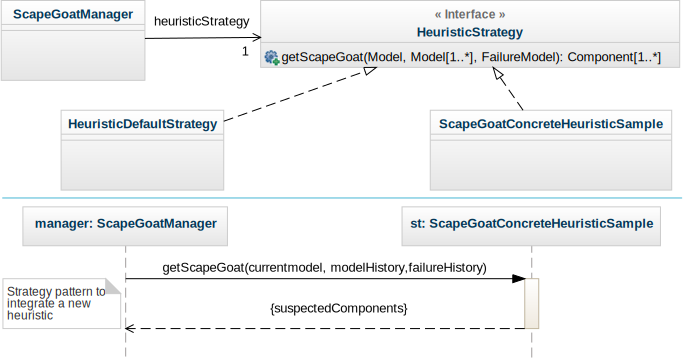
\includegraphics[width=0.9\textwidth]{chapter5/figures/strategy}
\caption{\label{fig:strategy}Scapegoat's extensibility}
\end{figure}

A second extensible aspect of the framework is the admission control system.
The framework provides an API to hook user-defined actions when new components are submitted for deployment.
Basic data describing the execution platform in terms of resource availability, information about the already deployed components and the new component's contract are sent to the user-defined admission control system.
On each request, the admission control system has to accept or refuse the new component.
In this paper, we are using an approach which check the theoretical availability of resources whenever a component is deployed, and accept the new component if the contract can fit in the remaining available resources.
ScapeGoat is meant to support other policies as, for instance, overcommitment.
 
A last element that can be specialized to user needs is the contracts semantic.
In section~\ref{componentcontract} we describe how we interpret the contract in this work.
However, it is possible to define other contract semantics, for instance, accepting values that are closed to the limit defined in the contract, or using fuzzy values instead of sharp values.
It is worth noting that modifying the semantic of the contract would likely involved redefining the domain-specific language to describe contract and also modifying the admission control system.

\subsubsection{Implementation strategy}
Scapegoat aims at minimizing monitoring overhead when the framework is running in \textit{Global Monitoring} mode. 
To achieve this, ScapeGoat removes as many monitoring probes as possible and only activates probes that are required.
This requires changing the bytecode that defines the application's classes at runtime, when the monitoring mode changes.
Bytecode is changed at a per-component basis.
We use the ASM library to perform bytecode manipulation and a Java agent to get access to and transform the classes.
Bytecode manipulation has been proposed before for resource accounting and profiling in Java \cite{binder_portable_2006,Binder200645,czajkowski_jres:_1998}.

The framework also proposes an on demand memory monitoring solution based on exploring the heap.
We built this solution on top of the JVM Tool Interface (JVMTI) by implementing the algorithms proposed in~\cite{Price:2003:GCM:829515.830545, Geoffray5270296}, with the main difference being that our solution works without modifying the garbage collector.
This makes our approach portable and allows it to work with different garbage collector implementations. 

\subsection{Leveraging Models@run.time to build an efficient monitoring framework}\label{sec:heuristic-based-on-modeling}

As presented in section \ref{monitorContainer}, our approach offers a dynamic way to activate and deactivate fine-grain localized monitoring.
We use a heuristic to determine which components are more likely to be faulty.
Suspected components are the first to be monitored.

Our framework can support different heuristics, which can be application or domain-specific.
In this paper we propose a heuristic that leverages the use of the Models@run.time approach to infer the faulty components.
The heuristic is based on the assumption that the cause of newly detected misbehavior in an application is likely to come from the most recent changes in the application.
This can be better understood as follows:
\begin{itemize}
\leftskip -.2in
  \item recently added or updated components are more likely to be the source of a faulty behaviour;
  \item components that directly interact with recently added or updated components are also suspected.
\end{itemize}

We argue that when a problem is detected it is probable that recent changes have led to this problem, or else, it would have likely occurred earlier.
If recently changed components are monitored and determined to be healthy, it is probable that the problem comes from direct interactions with those components.
Indeed, changes to interactions can reveal dormant issues with the components.
The algorithm used for ranking the components is presented in more detail in listing \ref{algo:heuristic}.
In practice, we leverage the architectural-based history of evolutions of the application, which is provided by the Models@run.time approach.


\begin{lstlisting}[escapeinside={(*}{*)},caption=The ranking algorithm (uses the model history for ranking).,label=algo:heuristic,float=!h]
ranker() : list<Component>
	visited = (*$\emptyset$*)
	ranking = {}
	for each model M (*$\in$*) History
		N = {c (*$\mid$*) c was added in M}
		Neighbors (*$ = \bigcup_{c \in N}{c.neighbors}$*)
		ranking.add N(*$\setminus$*)visited
		visited = visited (*$\cup$*) N
		SortedNeighbors = sort (Neighbors (*$\setminus$*) visited)
		ranking.add SortedNeighbors
		visited = visited (*$\cup$*) Neighbors
	return ranking
	
sort (S : Set<Component>) : list<Component>
	r = {}
	if (*$S \ne \emptyset$*)
		choose (*$b \mid b \in S$*) (*$\wedge$*) b is newer than any other element in S
		r.add b, sort (S(*$\setminus$*){b})
	return r
\end{lstlisting}

\section{ScapeGoat Performance Evaluation\label{sec:evaluation}}

In this section we present a first series of experiments and discuss the usability of our approach.
We focus on the following research questions to assess the quality and the efficiency of ScapeGoat:

\begin{itemize}
	\item \textbf{What is the impact of the various levels of instrumentation on the application?}
	Our approach assumes high overhead for full monitoring and low overhead for a lightweight global monitoring system. The experiments presented in section \ref{sec:OverheadFullMonitoring} show the overhead for each instrumentation level.
	\item \textbf{What is the performance cost of using instrumentation-based and heap-exploration-based memory monitoring?}
	Since both mechanisms have by design different features, the experiments in section \ref{sec:OverheadFullMonitoring} show the overhead each mechanism produces. 
	\item \textbf{Does our adaptive monitoring approach have better performance than state-of-the-art monitoring solutions?}
	The experiment presented in section \ref{sec:adaptive-vs-full} highlights the performances benefits of our approach considering a real-world scenario.
	\item \textbf{What is the impact of using a heuristic in our adaptive monitoring approach?}
	The experiment presented in section \ref{sec:switch-heuristic} highlights the impact of the application and component sizes, and the need of a good heuristic to quickly identify faulty components.
%Our last experiments aims at showing the potential benefits of the Heuristics in our approach. The experiment presented in section \ref{heuristic_eval} highlights the benefits of using a heuristics with a growing size of the application.
\end{itemize}

The efficiency of our monitoring solution is evaluated on two dimensions: the overhead on the system and the delay to detect failures.
We show there is a trade-off between the two dimensions and that ScapeGoat provides a valuable solution that increases the delay to detect a faulty component but reduces accumulated overhead.
This evaluation has been conducted on a Cyber Physical System case study.
It corresponds to a concrete application that leverage the Kevoree framework for dyamic adaptation purpose.

We have built several use cases based on a template application from our motivating example in section \ref{sec:motivatingexample}.
We reused an open-source crisis-management application for firefighters that has been built with Kevoree components.
We use two functionalities of the crisis-management application.
The first one is for managing firefighters.
The equipment given to each firefighter contains a set of sensors that provides data for the firefighter's current location, his heartbeat, his body temperature, his acceleration movements, the environmental temperature, and the concentration of toxic gases. 
These data are collected and displayed in the crisis-management application, which provides a global-view of the situation. 
The second functionality uses drones to capture real-time video from an advantageous point-of-view.

Figure \ref{fig:complete-usecase} shows the set of components that are involved in our use-case, including components for firefighters, drones and the crisis-management application\footnote{More information about these components is given in \url{http://goo.gl/x64wHG}}. The components in the crisis-management application are used in our experiments, but the physical devices (drones and sensors) are simulated through the use of mock components.
The application presents two components: the first one is a web browser that shows information about each firefighter in the terrain, and the second one allows to watch the video being recorded by any drone in the field.
A Redis database is used to store the data that is consumed for the application's GUI.

\begin{figure*}[!bt]
	\centering
	\includegraphics[scale=0.4]{./chapter5/figures/complete-usecase-new2}
	\caption{\label{fig:complete-usecase}The component configuration for our crisis-management use-case.}
\end{figure*}

Every use case we present extends the crisis-management base application by any one of the following possibilities: adding new or redundant components, adding external Java applications with wrapper components (e.g., Weka, DaCapo), or modifying existing components (e.g., to introduce a fault into them).
Using this template in the experiments allow us to measure the behavior of our proposal in a more realistic environment where many components with different features co-exist.
%is extended in every use case by: modifying existent components (e.g, to introduce faulty behavior), adding new redundant components and adding external java applications with a wrapper component.
%The particular features of each component are details in each experiment.

\subsection{Measurement Methodology} \label{sec:measurement_metodology}
To obtain comparable and reproducible results, we used the same hardware across all experiments: a laptop with a 2.90GHz Intel(R) i7-3520M processor, running Fedora 19 with a 64 bit kernel and 8GiB of system memory.
We used the HotSpot Java Virtual Machine version 1.7.0\_67, and Kevoree framework version 5.0.1.
Each measurement presented in the experiment is the average of ten different runs under the same conditions. 
%In addition to the template application we presented, we introduce a new component to execute an external jar file. This new component is used to measure the impact of the faulty behavior on the execution of the system by measuring its execution time.

The evaluation of our approach is tightly coupled with the quality of the resource consumption contracts attached to each component.
We built the contracts following classic profiling techniques. 
The contracts were built by performing several runs of our use cases, without inserting any faulty components into the execution.
Firstly, we executed the use cases in an environment with global monitoring activated to get information for the global contract.
Secondly, per-component contracts were created by running the use cases in an environment with full monitoring.

\subsection{Overhead of the instrumentation solution\label{sec:OverheadFullMonitoring}}
Our first experiment compares the various instrumentation levels to show the overhead of each one. 
In this section, \emph{Memory instrumentation} refers to the technique for accounting memory which leverage bytecode instrumentation, while \textit{Heap Exploration} refers to the memory accouting technique which leverage on-demand heap exploration.
%The results of the evaluation are fundamental because they justify the interest of our adaptative monitoring approach. 
%Additionally, these results are the baseline to understand the rest of the evaluation. 
In this experiment, we compare the following instrumentation levels: \emph{No monitoring}, \emph{Global monitoring}, \emph{Memory instrumentation}, \emph{Instructions instrumentation}, \emph{Memory and instructions instrumentation} (i.e., Full monitoring).
We also evaluate the impact on performance of the two fine-grain memory monitoring approaches we proposed: instrumentation-based and heap-dump-based.

In this set of experiments we used the DaCapo 2006 benchmark suite \cite{DaCapo:paper}. 
We developed a Kevoree component to execute this benchmark~\footnote{\url{http://goo.gl/V5T6De}}.
The container was configured to use full monitoring and the parameters in the contract are upper bounds of the real consumption\footnote{Scripts are generated from those available at \url{http://goo.gl/FR8LC7}.}.

\begin{figure}[!ht]
\centering
\begin{tikzpicture}
\begin{axis}[
every axis legend/.append style={nodes={right}},
ybar=0pt,
legend style={at={(0.25,1.1)},
anchor=north,legend columns=1, font=\tiny},
ylabel={Time (seconds)},
y label style={at={(0.04, 0.5)}},
scaled y ticks = false,
      y tick label style={/pgf/number format/fixed,
      /pgf/number format/1000 sep = \thinspace % Optional if you want to replace comma as the 1000 separator 
      },
xtick=data,ymin=0,
width = 13cm,
height = 5cm,
bar width = 6,
x tick label style={rotate=45,anchor=east, font=\small},
 axis lines*=left, % Don't display the top and right lines
 symbolic x coords={antlr,fop,hsqldb,jython,chart,luindex,xalan,lusearch}
]
\addplot[fill=black] coordinates 
	{(antlr,1.28) (fop,1.101) (hsqldb,2.337) (jython,2.351) (chart,2.534) (luindex,3.561) (xalan,1.224) (lusearch,1.305)};
\addplot[fill=gray] coordinates 
	{(antlr,1.023) (fop,1.039) (hsqldb,2.284) (jython,2.524) (chart,2.417) (luindex,3.165) (xalan,1.191) (lusearch,1.321)};
\addplot[pattern=north east lines] coordinates 
	{(antlr,2.164) (fop,1.188) (hsqldb,8.655) (jython,10.688) (chart,4.806) (luindex,8.001) (xalan,4.885) (lusearch,9.349)};
\addplot[pattern=crosshatch] coordinates 
	{(antlr,6.235) (fop,1.905) (hsqldb,9.091) (jython,10.905) (chart,8.985) (luindex,44.988) (xalan,8.026) (lusearch,9.261)};
\addplot[pattern=dots] coordinates 
	{(antlr,7.468) (fop,1.970) (hsqldb,15.888) (jython,18.625) (chart,11.502) (luindex,51.660) (xalan,11.188) (lusearch,18.975)};
\legend{No monitoring, Global monitoring, Memory instrumentation,Instructions instrumentation, Memory \& Instructions instrumentation}
\end{axis}
\end{tikzpicture}
\caption{Execution time for tests using the DaCapo Benchmark\label{overhead-of-monitoring}}
\end{figure}

Figure \ref{overhead-of-monitoring} shows the execution time of several DaCapo tests under different scenarios when only instrumentation is used to provide fine-grain monitoring.
First, we wish to highlight that Global monitoring introduces no overhead compared with the \emph{No monitoring} mode.
Second, the overhead due to memory accounting is lower than the overhead due to instruction accounting.
This is very important because, as we described in section \ref{monitorContainer}, memory probes cannot be deactivated dynamically.

To perform the comparison, we evaluate the overhead produced for each monitoring mode. We calculated the overhead as: \[overhead=\frac{WithInstrumentation}{GlobalMonitoring}\]

The average overhead due to instruction accounting is 5.62, while the value for memory accounting depends on the monitoring mechanism.
If bytecode instrumentation is used, the average overhead is 3.29 which is close to the values reported in \cite{Binder:2009:PPV:1464245.1464249}.
In the case of instruction accounting, these values are not as good as the values reported in \cite{Binder:2009:PPV:1464245.1464249}; because they obtain a better value between 3.2 and 4.3 for instructions accounting.
The performance difference comes from a specific optimization that we chose not to apply.
The optimization provides fast access to the execution context by adding a new parameter to each method.
Nevertheless, this solution needs to keep a version of the method without the new parameter because native calls cannot be instrumented like that. 
We decided to avoid such an optimization because duplication of methods increases the size of the applications, and with it, the memory used by the heap.
In short, our solution can reach similar values if we include the mentioned optimization, but at the cost of using more memory.
On the other hand, the values we report are far lower than the values reported in \cite{Binder:2009:PPV:1464245.1464249} for hprof.
Hence, we consider that our solution is comparable to state of the art approaches in the literature.

In figure~\ref{overhead-of-monitoring-with_heapexplorer} we compare the execution time of the same benchmarks but using different memory monitoring approaches.
This comparison is important because, as explained in section~\ref{monitorContainer}, the two approaches have different CPU footprint.
These are controlled experiments where, in order to stress the technique, we demand the execution of a \textit{heap exploration} step every two seconds, which is not the expected usage pattern.
On the contrary, the memory instrumentation technique is executed with the expected usage pattern.
In comparison to using memory instrumentation where the average execution time is 3.29, the average overhead in execution time  decreases to 1.79 if the \textit{Heap Exploration} monitoring mechanism is used.
This value is better than the value reported in \cite{Binder:2009:PPV:1464245.1464249}.
These results suggest that this technique has less impact on the behavior of applications being monitored.

\begin{figure}[!ht]
\centering
\begin{tikzpicture}
\begin{axis}[
every axis legend/.append style={nodes={right}},
ybar=0pt, legend style={at={(0.25,1.1)},
anchor=north,legend columns=1, font=\tiny},
ylabel={Time (seconds)},
y label style={at={(0.04, 0.5)}},
scaled y ticks = false,
      y tick label style={/pgf/number format/fixed,
      /pgf/number format/1000 sep = \thinspace % Optional if you want to replace comma as the 1000 separator 
      },
xtick=data,ymin=0,
width = \textwidth,
height = 5cm,
bar width = 6,
x tick label style={rotate=45,anchor=east, font=\small},
 axis lines*=left, % Don't display the top and right lines
 symbolic x coords={antlr,fop,hsqldb,jython,chart,luindex,xalan,lusearch}
]
% no monitoring
\addplot[fill=black] coordinates 
	{(antlr,1.28) (fop,1.101) (hsqldb,2.337) (jython,2.351) (chart,2.534) (luindex,3.561) (xalan,1.224) (lusearch,1.305)};
% memory
\addplot[pattern=north east lines] coordinates 
	{(antlr,2.164) (fop,1.188) (hsqldb,8.655) (jython,10.688) (chart,4.806) (luindex,8.001) (xalan,4.885) (lusearch,9.349)};
% heap dump
\addplot[pattern=crosshatch dots] coordinates 
	{(antlr,1.143) (fop,1.125) (hsqldb,8.639) (jython,2.762) (chart,2.836) (luindex,3.589) (xalan,1.822) (lusearch,5.078)};
% memory and instructions
\addplot[pattern=dots] coordinates 
	{(antlr,7.468) (fop,1.970) (hsqldb,15.888) (jython,18.625) (chart,11.502) (luindex,51.660) (xalan,11.188) (lusearch,18.975)};
% heap dump and instructions
\addplot[fill=white] coordinates 
	{(antlr,6.159) (fop,1.188) (hsqldb,14.647) (jython,10.950) (chart,9.059) (luindex,44.758) (xalan,7.812) (lusearch,15.990)};
% legend
\legend{No Monitoring, Memory instrumentation, Heap Exploration, Memory \& Instructions instrumentation, Heap Exploration \& Instructions Instrumentation}
\end{axis}
\end{tikzpicture}
\caption{Comparison of execution time for tests using two different memory monitoring techniques\label{overhead-of-monitoring-with_heapexplorer}}
\end{figure}

The results of our experiment shown in figures~\ref{overhead-of-monitoring} and~\ref{overhead-of-monitoring-with_heapexplorer} demonstrate the extensive impact of the \emph{Full monitoring} mode, which uses either \emph{Memory instrumentation} or \emph{CPU instrumentation}, has on the application. Thus, our \emph{Adaptive monitoring} mode, which uses \emph{Global monitoring} and switches to \emph{Full monitoring} or \emph{localized monitoring}, has the potential to reduce this accumulated overhead due to the fact that \emph{Global monitoring} has no appreciable overhead. 
%The results of the evaluation are fundamentals because they justify the interest of our adaptative monitoring approach. 
%Additionally, these results are the baseline to understand the rest of the evaluation. 

In addition, we plan to study alternatives to improve instruction accounting. %These alternatives are about using peak monitoring and learning monitoring.
For example, we plan to study the use of machine learning for monitoring \cite{tesauro2006hybrid}. Based on a machine learning approach, it is possible to train the monitoring system to do the instruction instrumentation. Then, instead of doing normal instruction instrumentation, we might only do, for example, method-calls instrumentation and with the learning data, the monitoring system should be able to infer the CPU usage of each call, whilst lowering the overhead.

\subsection{Overhead of Adaptive Monitoring vs Full Monitoring\label{sec:adaptive-vs-full}}
The previous experiment highlights the potential of using \emph{Adaptive monitoring}. However, switching from \emph{Global monitoring} to either \emph{Full} or \emph{Localized monitoring} introduces an additional overhead due to having to instrument components and activate monitoring probes.
Our second experiment compares the overhead introduced by the adaptive monitoring with the overhead of \emph{Full monitoring} as used in state-of-the-art monitoring approaches. 
%The result of this experiment shows the potential interest of the adaptive monitoring approach.

Table \ref{use-cases-sheet2} shows the tests we built for the experiment.
We developed the tests by extending the template application. Faults were introduced by modifying an existing component to break compliance with its resource consumption contract.
We reproduce each execution repetitively; thus, the faulty behaviour is triggered many times during the execution of the application. The application is not restarted.
%\hl{We selected as heuristic in almost every case \textit{number-of-failures} which is the best because there is only a single faulty component.}\todo{must be explain later}

\begin{table*}[!hb]
\centering
\caption{Features of use cases.\label{use-cases-sheet2}}
\begin{tabular}{|c|p{2.1cm}|p{1.4cm}|p{2cm}|p{2.5cm}|}
\hline Test Name & Monitored\newline Resource & Faulty\newline Resource & Heuristic & External Task \\ 
\hline UC1 & CPU, Memory & CPU & number\newline of failures & Weka, training neural network \\ 
\hline UC2 & CPU, Memory & CPU & number\newline of failures & dacapo, antlr \\ 
\hline UC3 & CPU, Memory & CPU & number\newline of failures & dacapo, chart \\ 
\hline UC4 & CPU & CPU & number\newline of failures & dacapo, xalan \\ 
\hline UC5 & CPU, Memory & CPU & less number\newline of failures  & dacapo, chart \\ 
\hline UC6 & Memory & CPU & number\newline of failures & Weka, training neural network \\ 
\hline 
\end{tabular} 
\end{table*}


Figure \ref{adaptive-vs-full} shows the execution time of running the use cases with different scenarios.
Each scenario uses a specific monitoring policy (\emph{Full monitoring}, \emph{Adaptive monitoring with All Components}, \emph{Adaptive monitoring with Localized monitoring}, \emph{Global monitoring}).
All these scenarios were executed with the heap explorer memory monitoring policy. 
This figure shows that the overhead differences between \textit{Full monitoring} and \emph{Adaptive monitoring with All Components} is clearly impacted by scenarios that cause the system to transition too frequently between a lightweight Global and a fine-grain Adaptive monitoring.
Such is the case for use cases UC3 and UC4 because the faulty component is inserted and never removed.
%As we explained in section \ref{analysis}, 
Using \emph{Adaptive monitoring} is beneficial if the overhead of \emph{Global monitoring} plus the overhead of switching back and forth to \emph{All Components monitoring} is less than the overhead of the \emph{Full monitoring} for the same execution period.
If the application switches between monitoring modes too often then the benefits of adaptive monitoring are lost.

The overhead of switching from \emph{Global monitoring} to \emph{full components} or \emph{Localized monitoring} comes from the fact that the framework must reload and instrument classes to activate the monitoring probes.
Therefore, using \emph{Localized monitoring} reduces the number of classes that must be reloaded.
This is shown in the third use-case of figure~\ref{adaptive-vs-full}, which uses a heuristic based on the number of failures.
Because we execute the faulty component many times, the heuristic is able to select, monitor and identify the faulty component quickly. This reduces overhead by 92.98\%. We use the following equation to calculate overhead:

\[ Gain=100-\frac{OurApproach-GlobalMonitoring}{FullMonitoring-GlobalMonitoring}*100 \]

We also evaluate the execution time for each use case using the instrumentation-based memory monitoring mode.
The average gain in that case is 81.49\% and, as shown in previous section, in average it behaves worse than the \textit{Heap Exploration} mechanism.
However, it is worth noting that the difference between using memory monitoring based on instrumentation and heap exploration is less remarkable than in the previous experiment.
Observe how in test UC4, using a combination of heap exploration and adaptive monitoring with all components behaves worse than using plain instrumentation-based memory monitoring.
In this particular test, activating and deactivating the monitoring probes dominate the execution time.
Alas, adding a heap exploration step right after the probes are activated, just add some extra overhead.
On the contrary, there is no additional step executed when we use instrumentation to measure the memory usage.
Apparently, what matter when the all components strategy is guiding the adaptive monitoring is the ratio among the amount of allocations performed by components and the size of those components.

\begin{figure}
\centering
\begin{tikzpicture}
\begin{axis}[
every axis legend/.append style={nodes={right}},
ybar=0pt, legend style={at={(0.8,1.2)},
anchor=north,legend columns=1, font=\tiny},
ylabel={Time (seconds)},
y label style={at={(0.04, 0.5)}},
scaled y ticks = false,
      y tick label style={/pgf/number format/fixed,
      /pgf/number format/1000 sep = \thinspace % Optional if you want to replace comma as the 1000 separator 
      },
xtick=data,ymin=0,
width = \textwidth,
height = 5cm,
bar width = 6,
x tick label style={rotate=45,anchor=east, font=\small},
 axis lines*=left, % Don't display the top and right lines
 symbolic x coords={UC1,UC2,UC3,UC4,UC5,UC6}
]
% full monitoring
\addplot[fill=black] coordinates 
	{(UC1,613.000) (UC2,46.363) (UC3,63.899) (UC4,78.324) (UC5,49.144) (UC6,132.949)};
% adaptive with all component
\addplot[fill=red, pattern=crosshatch dots] coordinates 
	{(UC1,432.744) (UC2,70.501) (UC3,198.554) (UC4,187.036) (UC5,32.340) (UC6,127.711)};
% adaptive with all component and heap dump
\addplot[fill=yellow, pattern=crosshatch] coordinates 
	{(UC1,410.790) (UC2,61.808) (UC3,95.503) (UC4,204.479) (UC5,16.864) (UC6,123.381)};
% adaptive with heuristic
\addplot[fill=green, pattern=north west lines] coordinates 
	{(UC1,176.413) (UC2,16.741) (UC3,29.461) (UC4,19.470) (UC5,27.001) (UC6,123.813)};
% adaptive with heuristic and heap dump
\addplot[fill=pink, pattern=dots] coordinates 
	{(UC1,169.467) (UC2,12.520) (UC3,16.403) (UC4,20.251) (UC5,15.110) (UC6,124.294)};
% global monitoring
\addplot[fill=cyan, pattern=north east lines] coordinates 
	{(UC1,166.759) (UC2,10.646) (UC3,14.37) (UC4,20.860) (UC5,14.77) (UC6,120.16)};
\legend{
	Full monitoring, 
	Adaptive with All Components using Memory Instrumentation, 
	Adaptive with All Components using Heap Exploration, 
	Localized monitoring using Memory Instrumentation, 
	Localized monitoring using Heap Exploration,
	Global Monitoring}
\end{axis}
\end{tikzpicture}
\caption{Execution time for some use cases under different monitoring policies.}\label{adaptive-vs-full}
\end{figure}

\subsection{Overhead from switching monitoring modes, and the need of a good heuristic\label{sec:switch-heuristic}}
As we explain in the previous experiments, even if using \emph{Localized monitoring} is able to reduce the overhead of the monitoring system, the switch between \emph{Global} and \emph{Localized monitoring} introduces additional overhead.
If this overhead is too high, the benefits of adaptive monitoring are lost.

In this experiment we show the impact of the application's size, in terms of number of components, and the impact of the component's size, in terms of number of classes, on adaptive monitoring. We also show that the choice of the heuristic to select suspected components for monitoring is important to minimize the overhead caused from repeated instrumentation and probe activation processes.

For the use case, we created two components and we introduced them into the template application separately.
Both components perform the same task, which is performing a \textit{primality test} on a random number and sending the number to another component.
However, one of the components causes 115 classes to be loaded, while the other only loads 4 classes.
%An additional component is in charge of generating random numbers to be consumed by the primality tester components.

We used the same basic scenario with a varying number of \textit{primality testing's} components and component sizes.
In this way, we were able to simulate the two dimensions of application size.
The exact settings, leading to 12 experiments, are defined by the composition of the following constraints:
\begin{itemize}
	\item $N_{comp} = \left\lbrace 4, 8, 16, 32, 64, 128 \right\rbrace$  which defines the number of components for the application
	\item $Size_{comp}=\left\lbrace 4, 115 \right\rbrace$ which defines the number of classes for a component
\end{itemize} 

With these use cases, we measured the delay to find the faulty component and the execution-time overhead caused by monitoring.
Figures \ref{fig:delay-time-115} and \ref{fig:delay-time-4} show the delay to detect the faulty component with regards to the size of the application.
In the first figure, the component size is 115 classes, and in the second figure, the component size is four classes.
%Figures \ref{fig:execution-time-many-115} and \ref{fig:execution-time-many-4} show the overhead of monitoring based on the execution time of the main task and according to the size of the application. In the first one, the component size is 115 classes and in the second one, the component size is four classes.

\input{./chapter5/delayTime}
\input{./chapter5/executionTimeManyComponents}

\subsubsection{Impact of the application size}
%\paragraph{Impact of the application size}
Using figures \ref{fig:delay-time-4} and \ref{fig:execution-time-many-4}, we see that the size of the application has an impact on the delay to detect faulty components, and also on the monitoring overhead.
We also calculated the time needed to find the faulty component with the \emph{All components} mode after its initialization (the time needed to switch from \emph{Global monitoring}).
This time is around 2 seconds no matter the size of the application.
That is the reason the switch from \emph{Global monitoring} to \emph{All components} has such a large effect on overhead.

These figures also show that using \emph{Localized monitoring} instead of \emph{All components} when switching from \emph{Global monitoring} helps reduce the impact of the application's size by reducing the number of components to monitor and the number of classes to instrument.
However, we also see that using a sub-optimal heuristic may have negatively impacted the delay to detect faulty components.
This can be explained by the multiple switches that the Random heuristic may often require to locate the faulty component.

\subsubsection{Impact of the component size}
%and \ref{fig:execution-time-many-115}, \ref{fig:execution-time-many-4}
In figures \ref{fig:delay-time-115} and \ref{fig:delay-time-4} we can observe that the component size greatly impact the performance and the delay for ScapeGoat to find the faulty comopnent. 
Similar to the explanation for the application's size, component size impacts the switch from \emph{Global monitoring} to \emph{Localized monitoring}, beacause of the class reloading and instrumentation.
A good heuristic rastically reduces the number of transitions; thus, it has a huge impact on the delay. 
When the components size increase, the choice of a good heuristics becomes even more important, because the cost of dynamic monitoring probes injection increase with the size of the components.

\subsection{Threats to validity}
Our experiments show the benefits of using adaptive monitoring instead of state-of-the-art monitoring approaches.
As in every experimental protocol, our evaluation has some bias which we have tried to mitigate.
All our experiments are based around the same case study. 
We have tried to mitigate this issue by using an available real case study.
We have also used different settings across our experiments, even if all of the experiments are based on the same case study.
Thus, our experiments limit the validity of the approach to applications with the same characteristics of the presented case study.
New experiments with other use cases are needed to broaden the validation scope of our approach.

The evaluation of the heuristic mainly shows the potential impact of using an ideal heuristic. 
More case study and experiments are needed to fully validate the value of our Models@run.time based heuristic.
\section{Scapegoat to spot faulty components in a scalable diverse web application}\label{sec:WebStudy}
In this section, we present another application that benefits from the Scapegoat approach.
Although the general goal of spotting components that behave abnormally regarding resource consumption remains the same, with this use case we highlight the possibility of using Scapegoat 
%on a real application 
%and a specific usage of Scapegoat 
to automatically find buggy components on a scalable modular web application.
The section \ref{MdMS} presents an introduction to the application use case, while the remainder of the section deals with the experimental setup and the results.


\subsection{Use case presentation}\label{MdMS}
We are applying the Scapegoat approach to check resource consumption contracts on a web application called MdMS.\footnote{\url{https://github.com/maxleiko/mdms-ringojs}}
This application offers a web Content Management System based on the Markdown language for editing posts. 
MdMS uses a typical architecture (as shown in Figure \ref{fig:webapp}) for scalable web applications: a load-balancer connected to a set of workers (called MdMS Sosie in the Figure \ref{fig:webapp}), which are themselves connected to a distributed database to retrieve the application specific content.
The worker layer of this application can be duplicated across various machines to support a growing number of clients.
The web application is currently online\footnote{\url{http://cloud.diversify-project.eu/}}. 

\begin{figure*}[!bt]
	\centering
	\includegraphics[scale=0.45]{./chapter5/figures/webapp2}
	\caption{\label{fig:webapp}Architecture of MdMS along with Scapegoat and additional components to adapt the system.}
\end{figure*}

The main characteristic of MdMS is that all workers are not pure clones but diverse implementations of the MdMS server stack~\cite{alliermulti}.
This proactive diversification of MdMS targets safety~\cite{avizienis85} and security~\cite{Forrest97} purposes.
In particular, we have used our recent technique for the automatic synthesis of \textit{sosie} programs~\cite{baudry2014tailored} in order to automatically diversify the workers. 
A \textit{sosie} is a variant of a program that exhibits the same functionality (passes the same test suite) and a diverse computation (different control or data flow). 
\textit{Sosie} synthesis is based on the transformation of the original program through statement deletion, addition or replacement.
%The MdMS application is leveraging this diversified set of workers in order to reach the scalability property while icluding diversity in the software layer to prevent the so-called BOBE (Blow Once, Blow Everywhere) attacks~\cite{alliermulti}.

While the construction of \textit{sosies} focuses on preserving functional correctness, it ignores all the non-functional aspects of the program.
Consequently, a \textit{sosie} offers no guarantee regarding its resource consumption and may contain memory leaks or other overhead on resource consumption that can significantly impact the performance of MdMS.

In this experiment, we use Scapegoat to monitor the resource consumption of the various \textit{sosies} of the MdMS workers.
This technique enables us to identify \textit{sosies} in a production environment that do not behave according to the resource consumption contracts, allowing the system to remove these workers and use other \textit{sosies}.
Our goal in this experiment is to answer the following question:

\begin{itemize}
 \item Does Scapegoat correctly identify the faulty components in a system which includes many variants of the same component?   
\end{itemize}

\subsection{Experimental setup}

We devised this experiment as a scenario where many clients interact with the web application at the same time by adding and removing articles.
The stress produced by these requests increases the resource consumption on the server side which is running on top of Kevoree components.
Figure~\ref{fig:webapp} depicts the server side's configuration.
Since MdMS is a web application developed on top of RingoJS~\footnote{\url{https://github.com/ringo/ringojs}}, a JavaScript runtime written in Java, our \textit{sosies} include the RingoJS framework and the application that has been wrapped into Kevoree components.

In this experiment, we deploy many of these components as back-end servers of the web application and we use Scapegoat to monitor the consumption of each server.
Their contracts regarding resource consumption were built using the mechanism described in section \ref{sec:measurement_metodology} but with the original MdMS worker as a reference component.
The application also contains a component acting as a front-end that evenly distributes the requests among back-end servers.
This load balancer implements a plain round robin policy.
%There is an additional component running on the platform, it is in charge of adapting the system.
%This component reacts to events produced by Scapegoat and modifies the deployed system following the Models@run.time paradigm.

To produce a realistic load on the web server we have recorded a set of standard activities on the MdMS web site using Selenium~\footnote{\url{http://www.seleniumhq.org/}}.
We then use the Selenium facilities to replay these activities many times in parallel to provide the required work load on the server.
% of resource consumption, we generate many accesses to the system.
%We use Selenium~\footnote{http://www.seleniumhq.org/} to accomplish this purpose since MdMS is a web application.
Our experimental settings feature 120 clients which are scheduled by a pool of 7 concurrent Selenium workers.
Each client adds 10 articles to the database through the Website GUI, which represents 16 requests per article, for a total of 19200 requests to the MdMS workers sent through the load balancer.
In this experiment, the Selenium workers are executed on the same physical device as the web server, with the same testing platform described in section~\ref{sec:measurement_metodology}.

The experiment is configured as follows.
Using the diversification technique described in~\cite{baudry2014tailored}, we synthesized 20 \textit{sosies} of the MdMS workers.
These \textit{sosies} are used to execute the application with a varying number of back-ends (from 4 to 10).
One particular \textit{sosie} has been modified by hand to ensure that it violates the original component's contract.
We execute all the described components as well as the Scapegoat components on a single instance of Kevoree.

\subsection{Experimentation results}

Figure~\ref{fig:execution-time-web-app} shows the time required on the server side to reply to all the requests sent by Selenium.
Although the values might look surprisingly high at first, they are in fact the result of a heavily loaded system.
Selenium is actually rendering a couple of web pages for each added article; hence at least 2400 pages are rendered.
Moreover, both clients and servers are sharing resources because they run on the same physical device.
%Another point to highlight is that the time needed to execute all these requests remains stable when no monitoring is used and only changes abruptly when deploying ten \textit{sosies}.
%The execution times remain stable when monitoring is not activated, which is expected because the number of requests does not change between experiments, the load balancer distributes these requests evenly, and we are using the same physical device to execute all back-end servers.
%The stability of the executions when monitoring is not activated is expected because the number of requests does not change between experiments, the load balancer distributes these requests evenly, and we are using the same physical device to execute all back-end servers.
This leads to very stable execution times when monitoring is not activated because the number of requests does not change between experiments, the load balancer distributes these requests evenly, and we are using the same physical device to execute all back-end servers.
%\todo{Please, read below the explanation for: Why the execution time decreases?}
In the \textit{local monitoring} series, the global time to execute decreases until reaching 9 \textit{sosies}.
Although counterintuitive, it is caused by the effect of having \textit{localized monitoring} and \textit{load balancing} at the same time.
For instance, when four \textit{sosies} are used, the monitoring probes are periodically injected into one component out of four, hence roughly a quarter of the requests are handled by a slower \textit{sosie}.
However, with eight components the slow execution path is only taken by around 12.5\% of the requests.
The overhead of \textit{Localized monitoring} when ten \textit{sosies} are deployed increases because the physical machine reaches its limit and begins thrashing.
As a consequence, low-level interactions with the hardware (e.g. cache misses), the operating system and the JVM slow down the execution.
On average, the overhead due to monitoring with both instruction instrumentation and memory instrumentation is 1.59, which is lower than the values shown in section~\ref{sec:OverheadFullMonitoring} for full monitoring despite only one of the instrumentation mechanisms being enabled in those experiments.
The values in this section are better even if we are monitoring both resources because we are using the adaptive approach.
   

\input{./chapter5/webAppResults}

In these experiments, we evaluate the accuracy of the output and its quality in terms of the time needed to find the faulty component.
Scapegoat always spots the correct \textit{sosie}.
It does so because it is an iterative process that continues until finding the faulty component.
In addition, Scapegoat does not output false positives during these experiments.
The delay to detect faulty components is shown in Figure~\ref{fig:delay-time-web-app}.
In this case, the values remain close to 2 seconds no matter the number of \textit{sosies} used nor the execution time.
This behavior is consistent with the experiments in section~\ref{sec:evaluation} because we are also using a good heuristic for the use case.
It shows that Scapegoat can spot faulty components with an acceptable delay in a real application.

\subsection{Discussion of the use case}
This use case shows that Scapegoat is able to provide useful information in real applications.
It also highlights how the framework can help select software variants at runtime in the context of software diversity.
Or, more generally, in the field of software oriented architectures where many stakeholders may provide the same services, Scapegoat can help to choose services.
Moreover, this use case leads to a distributed usage of Scapegoat, where the policies for admission control and resource consumption monitoring can be coordinated among distributed devices.

Finally, in systems where there are many variants of the same component or service, Scapegoat provides essential information to drive application reconfiguration.
For example, the adaptation component in Figure~\ref{fig:webapp} may use Scapegoat's faulty component selection to replace a faulty \textit{sosie} or to modify the scheduling policy in the load balancer.





%\section{Related work}\label{sec:related}

The Scapegoat framework is related to component monitoring, Models@run.time, component isolation and component performance prediction approaches.

Performance and resource-consumption prediction approaches are complementary to the Scapegoat framework because they can assist in better specifying the component contracts.
Some approaches require developers to provide extensive per-component metadata at design-time in order to calculate the application's overall performance or resource consumption \cite{Becker:2007:MPP:1216993.1217006,Jonge03scenario-basedprediction}.
Prediction approaches have been achieved by using combinations of design-time and runtime analyses \cite{autili2012hybrid}.
However, although many approaches to performance prediction have been proposed, none of them have obtained widespread use \cite{Koziolek:2006:QDD:2171366.2171393}.

%In \cite{Ghezzi2009}, the authors propose using performance models based on Queuing Networks to cope with the problem of architectural reasoning.
%The authors keep Models@run.time to enable re-estimation of model parameters based on the behavior of the running system and they present a mechanism to update the parameters when usage profiles change.
%The authors target the same problem we are dealing with, although we are not facing the prediction of behavior.

KAMI \cite{Ghezzi2009} builds performance models at design-time but uses and continually refines them at runtime.
By collecting runtime data, they are able to build performance and resource consumption models that reflect real usage.
They are able to adapt the application according to changes in components' behavior, but they do not use nor propose an adaptive monitoring system to minimize overhead.

%\todo{For Walter: Review this paragraph}
State of the art monitoring systems \cite{FrenotS04,KregerHaroldWilliamson03,Binder200645} extract steady data-flows of system parameters, such as, the time spent executing a component, the amount of I/O and memory used, and the number of calls to a component.
The overhead that these monitoring systems introduce into applications is high, which makes it unlikely for them to be used in production systems.
Maurel et al. \cite{Maurel:2012:AME:2304736.2304763} propose an adaptive monitoring framework for the OSGi platform.
Similar to our approach, they propose a global monitoring system that changes to a localized monitoring system when a problem is detected.
However, their work is focused on CPU usage and does not consider other resources, such as memory or I/O.
Exploring the Java heap to obtain useful information about resource consumption has been proposed in~\cite{Price:2003:GCM:829515.830545, Geoffray5270296}.
As in our work, they account objects to the resource principal being explored (in their case to OSGi bundles) the first time an object is reached.
Their solutions modify the garbage collector in order to reduce overhead, but this causes resource accounting to be tied to, and performed on, each collection cycle.
%but it means that the accounting step is performed on each collection cycle.
In contrast, our approach can be executed on demand, albeit at the cost of further passes over the heap.
%although our accounting step requires further passes over the heap, we can precisely specify when to execute it.

Gama and Donsez \cite{Gama:2010:SCS:2176905.2176915} propose using virtual machines in separate processes or using MVM isolates \cite{czajkowski2012multitasking} to manage trusted and untrusted components.
After an evaluation period, untrusted components can be moved to the trusted JVM if no problems are detected.
This allows the main application to depend on potentially faulty components without risking severe crashes.
We can also cite Microsoft technologies such as COM (Component Object Model) components which can be either loaded in the client application process or provided in an isolated process \cite{lowy2001and}.
In addition to process virtualization, some operating systems also propose user-space virtualization, which isolates not only the processes but also the memory, the network interface and the file system. Examples of these approaches are Jails\footnote{\url{http://www.freebsd.org/doc/handbook/jails.html}} for BSD, LXC\footnote{\url{http://lxc.sourceforge.net/}} and CGroups for Linux, and lmctfy\footnote{\url{https://github.com/google/lmctfy}}.
All of these approaches have the drawback of limiting code and instance sharing and introduce additional overhead in cross-boundary component interactions.
Furthermore, depending on the complexity of the approach, there is also overhead in having to manage multiple processes.

\section{Conclusions}\label{sec:conclusion}
In this chapter we presented Scapegoat, an adaptive monitoring framework to perform lightweight yet efficient monitoring of Component-Based Systems.
In Scapegoat, each component is augmented with a contract that specifies its resource usage, such as peak CPU and memory consumption.
Scapegoat uses a global monitoring mode that has low overhead on the system, and an on-demand fine-grained localized monitoring mode that performs extensive checking of the components' contracts.
The system switches from the global monitoring mode to the localized monitoring mode whenever a problem is detected at the global level in order to identify the faulty component.
Furthermore, we proposed a heuristic that leverages information produced by the Models@run.time approach to quickly predict the faulty components. 

Scapegoat has been implemented on top of the Kevoree component framework which uses the Models@run.time approach to tame the complexity of distributed dynamic adaptations.
The evaluation of Scapegoat shows that the monitoring system's overhead is reduced by up to 92.98\% in comparison with state-of-the-art full monitoring systems. 
The evaluation also presents the benefits of using a heuristic to predict the faulty component.
In the second part of the evaluation, we highlighted the benefit of Scapegoat on a classical web server architecture to dynamically determine faulty components.
This second example also exposes the capacity of Scapegoat to be applied to different application domains and confirms its relatively low overhead on the running system.
Scapegoat contributes to the state of the art by providing a monitoring framework which adapts its overhead depending on current execution conditions and leverages the architectural information provided by Models@run.time to drive the search for the faulty component.

The approach proposed in this chapter contributes to answer two research questions that were presented in the introduction of this thesis (see Section \ref{sec:intro-challenges}).
In particular, it answers \textit{\ref{rq:rq1}} (\textit{How can we provide portable and efficient support for resource consumption monitoring?}) by describing a monitoring framework that produces low performance overhead and is fully portable.
Likewise, our proposal partially answers \textit{\ref{rq:rq3}} (\textit{How can we leverage the knowledge about the architecture of applications to drive
a mechanism for resource management?}) by using knowledge about the structure of applications to drive the behavior of the framework.


\selectlanguage{english}
\chapter{Building Efficient Domain-Specific Memory Profilers}
\label{chp:dsl-memory}
\markboth{Building Efficient Domain-Specific Memory Profilers}{Chapter6}

\coolphrase{This is something here}{Fight Club}

%#Context  
%Domain-specific abstractions are increasingly used in industry to ease the development of applications. These abstractions take various forms, (e.g., domain-specific languages (DSL), macros, component models). Workbenches exist to define tooling over such abstractions. For example, DSL workbenches support the development of editors and code generators. 
% #Problem 
%However, profiling applications which use these abstractions requires significant development efforts to keep the traceability links between these abstractions and the runtime data-structures. This effort must be balanced with the limited audience of these abstractions. 
%Sate of the art profilers are able to represent such abstractions through generic query evaluation, but they suffer from bad performance issue. 

%#Contribution
%In this paper, we propose an approach to ease the development of efficient memory analysis tools to be used during the production stage.
%Our approach provides a DSL to express the mapping between abstractions and runtime data structure.
%At runtime, the generated  memory analysis tools leverage the object graph traversal mechanism to efficiently collect the specific memory data required.
%#Evaluation
%To evaluate our approach, we compare memory analysis tools produced with our DSL against: i) hand written optimized solutions, and ii) solutions based on existing tools which offer lower performance.
%The results show that our approach offers performance gain compared to previous solutions, and simplify the definition of memory analysis tools.

\lstset{
  aboveskip=5mm,
  belowskip=5mm,
  showstringspaces=false,
  columns=flexible,
  basicstyle=\color{black}\scriptsize,
  numbers=none,
  numberstyle=\color{gray}\scriptsize,
  keywordstyle=\color{black}\scriptsize\bfseries,
  commentstyle=\color{dkgreen}\scriptsize,
  stringstyle=\color{purple}\scriptsize,
  identifierstyle=\color{dkgray}\scriptsize,
  breaklines=true,
  breakatwhitespace=true,
  tabsize=4,
  captionpos=b,
}

\lstdefinelanguage{AlgLang}
{
literate={aaa}{bbb}3,
morekeywords={input, foreach, action, if, return, routine, values},
morekeywords={instances_for, have_id},
sensitive=true,
%frame=tblr,
morecomment=[l]{//},
morecomment=[s]{/*}{*/},
morestring=[b]",
}

\lstdefinelanguage{DSL}
{
literate={aaa}{bbb}3,
morekeywords={data, set_type, void, int, bool, Objects, THIS, is, ENTITY},
morekeywords={instances_for, have_names},
sensitive=true,
morecomment=[l]{//},
morecomment=[s]{/*}{*/},
morestring=[b]",
}

\lstdefinelanguage{OCL1}
{
literate={aaa}{bbb}3,
morekeywords={context,inv,and,or,self, if, not, else, endif, then},
sensitive=true,
frame=L,
morecomment=[l]{//},
morecomment=[s]{/*}{*/},
morestring=[b]",
xleftmargin=1\parindent,
}

\lstdefinelanguage{DSL2}
{
literate={aaa}{bbb}3,
frame=L, % tblr
%numbersep=2pt,
numbers=left,
numberstyle=\color{black}\scriptsize,
morekeywords={void, int, bool, in, is, or, and, struct, tableOf, ret},
morekeywords={membership, initialValues, updates, structure, initialObjects, create, using, constructor, foreach},
sensitive=true,
morecomment=[l]{//},
morecomment=[s]{/*}{*/},
morestring=[b]",
ndkeywords={false, true, this, referrer, threads, this_structure},
ndkeywordstyle=\color{blue}\bfseries,
xleftmargin=2\parindent
}

\lstdefinelanguage{OQL}
{
literate={aaa}{bbb}3,
numbers=left,
numberstyle=\color{black}\scriptsize,
morekeywords={SELECT, FROM, WHERE, UNION, AS, DISTINCT, ALL, GROUP, BY},
sensitive=true,
frame=tblr,
morecomment=[l]{//},
morecomment=[s]{/*}{*/},
morestring=[b]",
xleftmargin=1\parindent
}

\lstdefinelanguage{CYPHER}
{
literate={aaa}{bbb}3,
morekeywords={MATCH, RETURN, WITH, sum},
sensitive=true,
frame=tblr,
morecomment=[l]{//},
morecomment=[s]{/*}{*/},
morestring=[b]",
numbers=left,
numberstyle=\color{black}\scriptsize,
xleftmargin=1\parindent
}



The \gls{SLE} community aims at reducing the effort required in engineering new languages and their corresponding development tools, thus improving the efficiency of both people in charge of designing new languages and their users~\cite{sle}. 
However, as far as we know, they do not take into account profiling tools, which are essentials for software maintenance and optimization.
Indeed, although specific tools are needed to monitor running systems in order to detect defects or abnormal behaviors~\cite{duesterwald2000software, Jovic:2011:CMY:2076021.2048081},
little support exists to ease their creation.

In this chapter, we focus on the problem of easing the creation of memory profilers for domain-specific software abstractions that are designed to be executed on top of MRTEs. 
We first propose a metalanguage to specific what data about the memory use is of interest in a domain (see Section~\ref{sec:approach}).
A profiler is then generated to collect the data and present it in terms of concepts of that language. 
In addition, we present a tooled DSL based on such a metalanguage, which generates profilers for the JVM (see Section~\ref{sec:dsl-implementation}).
An important point of our approach is the low overhead induced by these profilers; this makes them usable in production environments (see Sections~\ref{sec:expressiveness} and~\ref{sec:dsl-evaluation}).

The contributions of this chapter are as follows:
\begin{itemize}
\item A metalanguage to describe what information a profiler must collect.
In addition, programs in this metalanguage also defines how to collect the information.
Although knowledge of the underline execution model is required, the procedure to obtain data is mostly defined without using low-level details.  

\item A concrete implementation of this metalanguage that target the JVM.
In particular, by using the \glslink{JVMTI}{JVMTI}, we are able to generate memory profilers with low overhead.
Concrete profilers already generated are portable to any implementation of the JVM that supports JVMTI.

\item A discussion of the metalanguage's expressiveness, and an evaluation of the performance overhead induced by three profilers in real-world use cases.
\end{itemize}

%\section{Motivating example}\label{sec:scapegoat-motivaing-example}

%\subsection{Motivating example\label{sec:motivatingexample}}

%In this section we present a motivating example for the use of an optimistic adaptive monitoring process in the context of a real-time crisis management system in a fire department. 
During a dangerous event, many firefighters are present and need to collaborate to achieve common goals.
%In a situation where many firefighters are present and need to collaborate to handle a dangerous event, 
Firefighters have to coordinate among themselves and commanding officers need to have an accurate real-time view of the system.

The Daum project\footnote{\url{https://github.com/daumproject}} provides a software application that supports firefighters in these situations.
The application runs on devices with limited computational resources because it must be mobile and taken on-site.
%As the software have to be mobile to take it on site, it is running on devices with limited computation resources.
It provides numerous services for firefighters depending on their role in the crisis.
In this chapter, we focus on the two following roles:
\begin{itemize}
\leftskip -.2in
 \item A collaborative functionality that allows commanding officers to follow and edit tactical operations. The firefighters' equipment include communicating sensors that report on their current conditions.
 \item A drone control system which automatically launches a drone equipped with sensors and a camera to provide a different point-of-view on the current situation.
\end{itemize}

%\todo{I don't get this for example. It is not relate to the previous sentence.}For example, one service is related to firefighter information monitoring to know the location, activity and health status of each firefighter involved on the crisis but also to get some information on their environment (e.g. temperature, toxic gas). Another service is in charge of the management of victims. They must be redirected according to their needs.

As is common in many software applications, the firefighter application may have a potentially infinite number of configurations. These configurations depend on the number of firefighters involved, the type of crisis, the available devices and equipment, among other parameters. 
Thus, it is generally not possible to test all configurations to guarantee that the software will always function properly. 
Consequently, instead of testing all configurations, there is a need to monitor the software's execution to detect faulty behaviours and prevent system crashes. 
However, fine-grained monitoring of the application can have excessive overhead that makes it unsuitable with the application and the devices used in our example.
Thus, there is a need for an accurate monitoring system that can find faulty components while reducing overhead.

The Daum project has implemented the firefighter application using a Component Based Software Architecture.  The application makes extensive use of the Kevoree\footnote{\url{http://www.kevoree.org}\label{note:kevoree}} component model and runtime presented in chapter \ref{chap:abstractions_and_resource_management}.

% Using our adaptive monitoring solution, we are able to reduce the overhead of the monitoring process keeping enough well response time to find faulty behaviors.



\section{Kevoree Component Model}

Kevoree~\footnote{\url{http://kevoree.org/}} is an execution platform for distributed software systems.
It is built around a component model, and it leverages the model@runtime approach to ease the construction of reconfigurable systems.

Built on top of dynamic component frameworks, Models@run.time denote model-driven approaches that aim at taming the complexity of dynamic adaptation.
It basically pushes the idea of reflection~\cite{morin09a} one step further by considering the reflection-layer as a real model: ``something simpler, safer or cheaper than reality to avoid the complexity, danger and irreversibility of reality''.
In practice, component-based and service-based platforms offer reflection APIs that allow instrospecting the application (e.g., which components and bindings are currently in place in the system) and dynamic adaptation (e.g., changing the current components and bindings).
While some of these platforms offer rollback mechanisms to recover after an erroneous adaptation~\cite{leger2010reliable}, the purpose of Models@run.time is to prevent the system from actually enacting an erroneous adaptation. 
In other words, the ``model at runtime'' is a reflection model that can be decoupled from the application (for reasoning, validation, and simulation purposes) and then automatically resynchronized.
This model can not only manage the application's structural information (i.e., the architecture), but can also be populated with behavioural information from the specification or the runtime monitoring data.

Kevoree provides multiple concepts that are used to create a distributed application that allows dynamic adaptation. The \emph{Node} concept is used to model the infrastructure topology and the \emph{Group} concept is used to model the semantics of inter-node communication, particularly when synchronizing the reflection model among nodes. 
Kevoree includes a \emph{Channel} concept to allow for different communication semantics between remote \emph{Components} deployed on heterogeneous nodes. 
All Kevoree concepts (\textit{Component}, \textit{Channel}, \textit{Node}, \textit{Group}) obey the object type design pattern~\cite{johnson_type_1997} in order to separate deployment artifacts from running artifacts.  

%Platforms
Kevoree supports multiple execution platforms (e.g.,~Java, Android, MiniCloud, FreeBSD, Arduino). For each target platform it provides a specific runtime container. 
%Tools
Moreover, Kevoree comes with a set of tools for building dynamic applications (a graphical editor to visualize and edit configurations, a textual language to express reconfigurations, several checkers to valid configurations). 

As a result, Kevoree provides a promising environment by facilitating the implementation of dynamically reconfigurable applications in the context of an open-world environment.
Because our goal is to design and implement an adaptive monitoring system, the introspection and the dynamic reconfiguration facilities offered by Kevoree suit the needs of the ScapeGoat framework.

\begin{comment}
\subsection{Kevoree}
Kevoree is an open-source dynamic component platform, which relies on Models@run.time~\cite{BlairBF09} to properly support the dynamic adaptation of distributed systems.
Our use case application and the implementation of the Scapegoat framework make extensive use of the Kevoree framework.
The following subsections detail the background on component-based software architecture, introduce the Models@run.time paradigm and give an overview of the Kevoree platform.

\subsubsection{Component-based software architecture}

Software architecture aims at reducing complexity through abstraction and separation of concerns by providing a common understanding of component, connector and configuration~\cite{xadl,Medvidovic:2000,VanOmmering-et-al-00}.
One of the benefits is that it facilitates the management of dynamic architectures, which becomes a primary concern in the Future Internet and Cyber-Physical Systems~\cite{DBLP:journals/ase/NittoGMPP08, Johnson:2015:CSM:2735960.2735979}.
Such systems demand techniques that let software react to changes by self-organizing its structure and self-adapting its behavior~\cite{PanzicaLaManna:2012:LDU:2304736.2304764, Johnson:2015:CSM:2735960.2735979, Zhang:2009:MVD:1509239.1509262}.
Many works~\cite{cbse-conference} have shown the benefits of using component-based approaches in such open-world environments~\cite{baresi2006toward, Caporuscio:2010:AIA:1985522.1985547, Perez-Palacin:2010:PAO:1712605.1712614}.

To satisfy the needs for adaptation, several component models provide solutions to dynamically reconfigure a software architecture through, for example, the deployment of new modules, the instantiation of new services, and the creation of new bindings between components~\cite{Porter:2014:RMC:2602458.2602471, Zheng:2014:RCC:2679601.2680405, Irmert:2008:RAS:1370018.1370036, Ghezzi:2010:QDD:2163764.2163774}. 
In practice, component-based (and/or service-based) platforms like Fractal~\cite{bruneton06}, OpenCOM~\cite{BlairCULJ04}, OSGi~\cite{OSGI:r5} or SCA~\cite{SEINTURIER:2011:INRIA-00567442:1} provide platform mechanisms to support dynamic architectures.

%As a result, component-based platforms offer a challenging playground for building adaptive monitoring framework as they raise a new challenge in easing the open-world paradigm and they can be an element of the solution. 

%In this context, traditional software development, based on the closed-world assumption that the  boundary between system and environment is known and unchanging does not work.


\subsubsection{Models@run.time}
Built on top of dynamic component frameworks, Models@run.time denote model-driven approaches that aim at taming the complexity of dynamic adaptation.
It basically pushes the idea of reflection~\cite{morin09a} one step further by considering the reflection-layer as a real model: ``something simpler, safer or cheaper than reality to avoid the complexity, danger and irreversibility of reality''.
In practice, component-based and service-based platforms offer reflection APIs that allow instrospecting the application (e.g., which components and bindings are currently in place in the system) and dynamic adaptation (e.g., changing the current components and bindings).
While some of these platforms offer rollback mechanisms to recover after an erroneous adaptation~\cite{leger2010reliable}, the purpose of Models@run.time is to prevent the system from actually enacting an erroneous adaptation. 
In other words, the ``model at runtime'' is a reflection model that can be decoupled from the application (for reasoning, validation, and simulation purposes) and then automatically resynchronized.
This model can not only manage the application's structural information (i.e., the architecture), but can also be populated with behavioural information from the specification or the runtime monitoring data.


\subsubsection{The Kevoree framework\label{sec:kevoree}}	
% Se proteger un peu plus sur Kevoree pour big node / placer plus de ref / comparaison ?
%Language

%\todo{THIS SECTION IS VERY UNCLEAR!!!}

Kevoree provides multiple concepts that are used to create a distributed application that allows dynamic adaptation. The \emph{Node} concept is used to model the infrastructure topology and the \emph{Group} concept is used to model the semantics of inter-node communication, particularly when synchronizing the reflection model among nodes. 
Kevoree includes a \emph{Channel} concept to allow for different communication semantics between remote \emph{Components} deployed on heterogeneous nodes. 
All Kevoree concepts (\textit{Component}, \textit{Channel}, \textit{Node}, \textit{Group}) obey the object type design pattern~\cite{johnson_type_1997} in order to separate deployment artifacts from running artifacts.  

%Platforms
Kevoree supports multiple execution platforms (e.g.,~Java, Android, MiniCloud, FreeBSD, Arduino). For each target platform it provides a specific runtime container. 
%Tools
Moreover, Kevoree comes with a set of tools for building dynamic applications (a graphical editor to visualize and edit configurations, a textual language to express reconfigurations, several checkers to valid configurations). 

%The remainder of this section describes the main concepts of the Kevoree component model that are useful to understand the scapegoat approach.
%\todo{One sentence to explicit how Kevoree and Model@Runtime help the development of our approach}

As a result, Kevoree provides a promising environment by facilitating the implementation of dynamically reconfigurable applications in the context of an open-world environment.
Because our goal is to design and implement an adaptive monitoring system, the introspection and the dynamic reconfiguration facilities offered by Kevoree suit the needs of the ScapeGoat framework.
%As a result, component-based platforms offer a challenging playground for building adaptive monitoring framework as they raise a new challenge in easing the open-world paradigm and they can be an element of the solution. 



%\subsection{Dynamic Adaptation with Kevoree}
%Kevoree aims at providing advanced adaptation capabilities to different types of nodes:
%\begin{itemize}
%\setlength{\itemsep}{0pt}
%\setlength{\parskip}{0pt}
%\setlength{\parsep}{0pt}
%\item 
%\noindent{\bf Level 1: Parametric adaptation.} Dynamic update of parameter values, e.g. change of sampling rate in a component that wraps a physical sensor (adaptation of instance properties).

%\item 
%\noindent{\bf Level 2: Architectural adaptation.} Dynamic addition or removal of bindings or components, e.g. replication of software components and channels on different nodes to perform load balancing (adaptation of instances graph).

%\item 
%\noindent{\bf Level 3: Dynamic provisioning of types.} Hot deployment of component types that were not foreseen before the initial deployment of the system. 
%This allows for system evolution by enabling parametric and architectural reconfigurations, including management of instances for types that are added and managed dynamically (adaptation of types).

%%\item 
%%\noindent{\bf Level 4: Adaptation for remote management.} Nodes supporting level~4 adaptation participate in a remote management layer, which supervises less powerful nodes. 
%%This layer monitors remote nodes by requesting their current Kevoree model;
%%the layer triggers dynamic adaptation of nodes by sending precomputed reconfiguration scripts to them. 
%%This remote adaptation process supports seamless management of less powerful nodes by a more powerful one, which has enough resources to build and evaluate new and appropriate  configurations.
%\end{itemize}

%The adaptation engine relies on a model comparison between two Kevoree models to compute a  script for a safe system reconfiguration; execution of this script brings the system from its current configuration to the new selected configuration~\cite{morin09a}. 
%Model comparison yields  a delta-model defining changes (using CRUD operations) that should be applied on the source model to obtain the target model. 
%Planification algorithms~\cite{daubert} use this delta-model as input in order to defined an efficient schedule of the adaptation steps. 
%The delta-model is finally compiled into a Kevoree script. 
%The Kevoree Script language (KevScript for short) is a core language for describing reconfiguration.
%KevScript  is comparable to FScript for Fractal Component Model~\cite{DBLP:journals/adt/DavidLLC09}. 
%Execution of a KevScript directly adapts a Kevoree system, without the need for  a full Kevoree model definition. 
%Such adaptation scripts are written by designers, or they can be generated  by automated processes ({\em e.g.} within a  control loop managing the Kevoree system).

%\hl{(Johann) What is the point of having so much detail about the Kevoree adaptation framework for this paper? It's not clear to me or we should have a last paragraph explaining a bit in what this is usefull for the rest of the paper.}

\end{comment}


%\section{Motivating example}\label{sec:motivation}
%For the motivating example talk about the case of online memory consumption monitoring.
%Explain how it is useful to perform the monitoring stage of the MAPE Loop.
%Explain the particular case of Component-Based Software Systems built on top of Java (e.g. OSGi, Kevoree)
Online application performance monitoring is a very important concern to detect misbehavior, failures or even potential attacks.
%Self-adaptive and autonomic systems~\cite{kephart2003vision} are systems capable of dynamically adapting their behavior in reponse to changes in their execution environment (failure, performance degradation and so on).
%Self-adaptive systems are generally following a standard architecture called the MAPE-K loop~\cite{Huebscher:2008:SAC:1380584.1380585} which stand for
%Monitoring, Analysis, Planning and Execution.
%Monitoring is the step where the control loop collects meaningful information to drive the system adaptations.
%A self-adaptive system must thus collect data regarding computational resource consumption in order to be resource-aware~\cite{Maheo:2004:MSD:1018420.1019675, Simao:2012:VEJ:2310096.2310158, Guidec:2003:JMP:1899290.1899304}.
At the same time, online memory usage monitoring and analysis is a complex problem when the application development has leveraged specific abstractions. 
This section discusses three motivating examples in which developers use specific abstractions provided by a framework or by himself. 
For each of these examples, we illustrate the mismatch between the concepts used by developers and the concepts manipulated by the state of the art profiling tools. 

Our first example leverage the use of active annotations in the XTend~\cite{bettini2013implementing} language.
Active annotations allow developers to participate in the translation process of Xtend source code to Java code via library.
This is particularly useful when Java requires to write a lot of boilerplate manually. 
For instance, many of the good old design patterns fall into this category. 
An active annotation is an annotation declared either in Java or Xtend, which is itself annotated with Active. 
\textit{@Active} takes a type literal as a parameter pointing to the processor. 
It can be seen as a subset of macro mechanism that exists in Scala or smalltalk~\cite{burmako2013scala}. 
Such mechanism is often used directly by developers to introduce their own abstraction or defining their own internal DSL. 
For example, in the K3-AL\footnote{Available at https://github.com/diverse-project/k3/wiki} project, we use active annotations to create an open-class mechanism in Java~\cite{Clifton:2000:MMO:353171.353181}. 
As a result, the annotation processor change the program structure to implement this feature. 
It adds some methods indirection (to $AASpect$), create new set of objects that represents the state of one conceptual object ($AASpectProperty$), use the Xtend extension method feature, etc\dots 
Figure~\ref{fig:famous} shows the result of this translation process. 
The left part illustrates the code written by the developer, the middle part shows the developer view (the code that can be written to use the open-class mechanism), the right part describes the runtime view. 
 
The current issue is the lack of traceability in the translation process. 
As a result, the abstraction used by the profiler does not match the abstractions used by the developer. 
Adapting profiling tools for these abstractions still requires significant development efforts that must be balanced with the limited audience of these abstractions.

\begin{figure*}
\centering
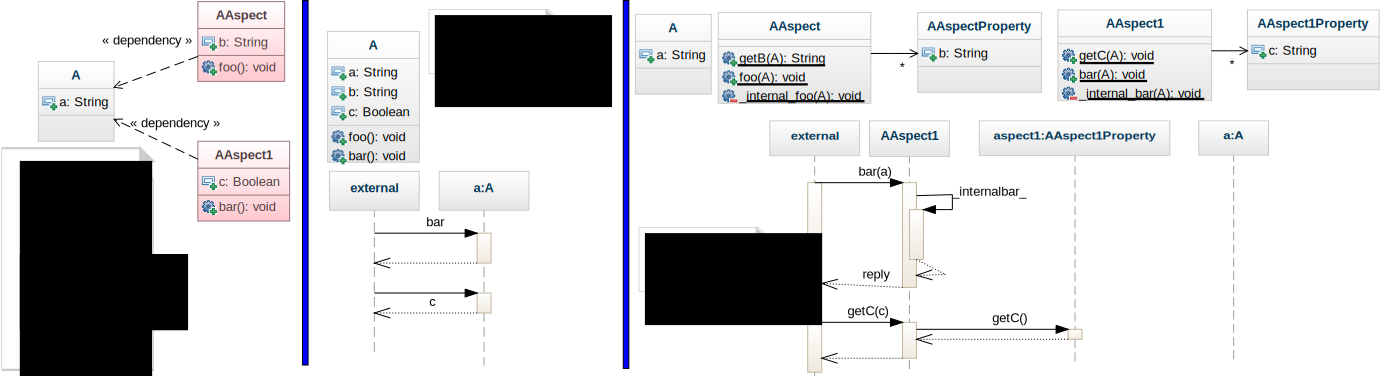
\includegraphics[width=0.9\linewidth]{chapter6/fig/famous}
\caption{Translation process used for building developer abstraction using annotations}
\label{fig:famous}
\end{figure*}

An other example is the OSGi framework. 
In OSGi, developers and users deploy many bundles on top of a single JVM.
It is therefore very complex to decide which bundle should be accounted for the consumption of a particular object because the heap is shared by all the bundles.
A solution to this problem is to account an object $O$ to a bundle if the object $O$ was loaded using the classloader $C$ associated with such a bundle: you can find a path from $C$ to $O$ in the graph of live objects.
This particular solution can be implemented because the mapping between bundle and Java abstractions is known. 
Hence, we can hard-code this mapping in a specific profiler written in JVMTI or we can modify the garbage collector.
Nonetheless, different component-models implementations may map components to different Java abstractions; therefore, the previous solution does not work for all of them.
Thus developers have to design and implement specific profilers from scratch for all the framework and specific abstractions they are using. 
This is a very error prone, hard to debug and time consuming task. 

Finally, the Spring Framework provides a comprehensive programming and configuration model for modern Java-based enterprise applications - on any kind of deployment platform. 
A key element of Spring is its infrastructural support at the application level.
Spring focuses on all the repetitive manual tasks a developer has to handle when developing enterprise applications so that teams can focus on the business logic, without unnecessary ties to specific deployment environments. 
To take care of all these repetitive tasks, Spring provides Dependency Injection, Aspect-Oriented Programming including Spring's declarative transaction management, RESTful web service framework, support for JDBC, JPA, JMS, \dots. 
For all these features, Spring provides abstractions through Java annotations for developers, injects at runtime dynamic proxies to handle these repetitive tasks and adapts the wiring of objects. 
As a result, it exists a mismatch between the running set of objects and the application design. 
This mismatch makes the application profiling difficult and error prone. 


\section{Approach}\label{sec:approach}

In this chapter, we propose a tool to create custom memory profilers for MRTEs.
We are interested on easing the task of defining new profilers without sacrificing their performance regarding CPU consumption.
Keeping the profiler's overhead as low as possible is of utmost importance for us because lightweight profilers can be use both during the development phase and during the application execution in a production environment.
To reach this goal, we propose a Domain Specific Language (DSL) and its code generator which aims at describing and generating efficient online memory profilers. 

We next present the syntax, semantics and usage examples of our domain-specific language.


\subsection{Brief overview of the domain}

Memory profilers aim at capturing information regarding how an application use memory.
In an object-oriented runtime environment such as Java, this information can be as simple as the number of objects of a specific class, but it can also be  as complex  as the list of possible memory leak sources.
Along this paper, the term memory profiler refers to any kind of process to retrieve data about the memory usage.
Some examples include: computing the number of objects reachable from a specific class object; finding out if there is an instance of class $A$ which is referencing an instance of class $B$.
A last example could be computing for each instance of the class \textit{String} its length and the number of references to it.
It is worth mentioning that the data collected by a profiler may have an arbitrary type.
For instance, in the previous examples the types are primitives integer, boolean and a non-primitive type.

%The rest of this section introduces the vocabulary we use in the domain of memory profilers.

In this paper, we are interested in \textbf{\textit{objects}} as in object-oriented programming.
We also see an \textit{object} as an atomic entity that consumes memory to store the values of its attributes.
We have  reduced the available operations on objects to: accessing attributes, obtaining the amount of memory used to represent the object, and accessing meta-data such as the class name.

The \textbf{\textit{memory heap}} is the region of memory used to store dynamically allocated \textit{objects}.
Although this concept is pervasive in general purposes programming languages, we are only interested on MREs such as Java where every \textit{object} must be allocated in this region.

A \textbf{\textit{structure}} is an important concept in our domain.
It consists of a set of related \textit{objects} in the \textit{memory heap}.
The smallest non-empty \textit{structure} we can consider, is a structure containing a single object.
The \textit{memory heap} is the universe of objects and each \textit{structure} is a subset of this universe.

A \textbf{\textit{memory profile}} is a value associated to a \textit{structure} which can be derived out of the indivdual \textit{objects} included in the \textit{structure}. 
An example of useful derived value for a \textit{structure} is its total size: $\textit{total\_size(S)} = \sum_{o \in S} {sizeof(o)}$.
A common usage is to identify many \textit{structures} in the heap to obtain a \textit{memory profile} for each of them.
These two steps: identifying \textit{structures} and computing their \textit{memory profile} correspond to what we call \textbf{\textit{memory profiling}}. 

Finally, a \textbf{\textit{structure type}} provides a description of the behavior of a set of \textit{structures}. 
In particular, it provides (i) a function to evaluate whether an object is member of the \textit{structure}, (ii) a way to define the values corresponding to the \textit{memory profile} of the \textit{structure}, and finally (iii) a factory to identify all  corresponding \textit{structures} in the \textit{memory heap}.

\subsection{Abstract Syntax}\label{sec:abstract-syntax}

The metamodel shown in Figure~\ref{fig:as} describes the abstract syntax of our DSL.
The main concept of this metamodel is a \textit{CustomProfiler} which is composed of \textit{UserDefined} types and a \textit{StructureFactory}.
The concepts related to \textit{UserDefined} types are shown on the left part of the metamodel, while the right part describes the \textit{StructureFactory} which represents both the set of  structures to identify and the value to compute on these structures.

\subsubsection{User-defined types}
In addition to various \textit{BasicTypes} such as \textit{Integer}, \textit{String} and \textit{Boolean}, the language supports the definition of both \textit{Records} and \textit{Lists}.
As expected, a \textit{record} contains \textit{fields} to hold values of previously defined types.
Likewise, a \textit{list} refer to a \textit{base type}; hence all the members of a list must be of the same type.
In a custom profiler, \textit{UserDefined} types can be composed in arbitrary ways as long as no type contains a recursive declaration.
We can formalize such a constrain using OCL (Object Constraint Language~\footnote{http://www.omg.org/spec/OCL/}):

\begin{lstlisting}[escapeinside={(*}{*)},
label=fig:membership,
language=OCL, frame=tblr]
context Record inv: 
   not fields->oclAsSet()->closure(t)->exists(t | t = self)

context List inv:
   not baseType->oclAsSet()->closure(t)->exists(t | t = self)
\end{lstlisting} 

A \textit{List} has operations to manipulate any value which represent a list.
Figure~\ref{fig:as} shows a subset of these operations.
In general, these operations correspond to the set of \textit{standard} operations of any implementation of the list data type.

\subsubsection{Defining structures to profile}
Defining the \textit{StructureFactory} is the core of writing a custom profiler.
A \textit{StructureFactory} contains an \textit{Expression} through the \textit{instances} relationship which indicates a pattern to identify structures in the memory heap.
Notice that a single instance of \textit{StructureFactory} creates many data structures in memory; thus the \textit{Expression} corresponds to a list indicating that a new structure must be instantiated for each element of the list.
Forcing the \textit{Expression} to be a \textit{List} can be easily formalized using OCL:

\begin{lstlisting}[escapeinside={(*}{*)}, label=fig:instances, language=OCL, frame=tblr]
context StructureFactory inv: instances.type.oclIsTypeOf(List)
\end{lstlisting}

Defining a new \textit{StructureFactory} implies defining its \textit{type} which is an instance of \textit{StructureType}.
This concept describes the mechanism used to populate, out of objects, a structure and its information.
In short, each structure in memory instanciated through a \textit{StructureFactory} has a type \textit{StructureType}.
For example, we may be interested in finding all the \textit{SimplyLinkedList} in the memory snapshot depicted in Figure~\ref{fig:simple_snapshot}.
In such a case, there are two \textit{SimplyLinkedList}, but we only need one mechanism to identify them because they have the same pattern in memory. 

\begin{figure*}
\centering
\includegraphics[width=0.87\linewidth]{chapter6/fig/AS}
\caption{Custom profiler Metamodel}
\label{fig:as}
\end{figure*}

\begin{figure}
\centering
\includegraphics[width=0.65\linewidth]{chapter6/fig/lists}
\caption{Memory snapshot with three linked lists}
\label{fig:simple_snapshot}
\end{figure}

A \textit{StructureType} is composed of \textit{Assignments} that are used as \textit{initialValues} for each \textit{Variable} holding information - similar to a constructor in object-oriented programming.
Once a new structure is created, the \textit{Assignments} are executed to assign the initial value of each \textit{Variable}.
Observe that \textit{variables} do not refer to a \textit{Type}.
Our DSL is strongly typed and the \textit{type} of each user-defined variable is inferred from its initial value.
Nevertheless, there is a built-in variable in each \textit{StructureType} that is only accessible during initialization.
Its type is predetermined as part of the language specification.
We force the use of the proper type using OCL:

\begin{lstlisting}[escapeinside={(*}{*)}, label=fig:instances, language=OCL, frame=tblr]
context StructureType inv:  initialValues->exists(a: Assignment | 
     a.lvalue.name = 'initialObjects' and a.rvalue.type.oclIsTypeOf(List)
   ) 
\end{lstlisting}

In addition, a \textit{StructureType} contains a boolean \textit{expression} which is the \textit{membership function} used to decide whether an object should be included in the structure instance.
Finally, it also contains a set of \textit{Assignments} to update the value of each \textit{variable} every time a new object is included in the structure.
This set of \textit{Assignments} is used to compute the actual value of the memory profile.
The major constraint regarding these \textit{updates} is that they must refer to already initialized \textit{variables} and the new assigned values must match the previous types.
We formalize such a constrain using OCL:

\begin{lstlisting}[escapeinside={(*}{*)}, label=fig:lvalue, language=OCL, frame=tblr]
context StructureType inv:  updates->forAll(a: Assignament | 
    self.initialValues->exists(aa : Assignament | 
       aa.lvalue = a.lvalue and aa.rvalue.type = a.rvalue.type
     ))
\end{lstlisting}

In our DSL, \textit{expressions} play a big role.
For the sake of readability, Figure~\ref{fig:as} only shows a couple of concepts related to them.
However, it is noteworthy that, in addition to \textit{arithmetic}, \textit{boolean} and \textit{literals} for basic types, the language includes lambda expressions, literal for records and lists.
Moreover, the language defines \textit{built-in rvalues} which are nothing but expressions initialized by the runtime within a specific scope.
Instead of being user-defined, the types of these expressions are also defined by the runtime.
There are two types of \textit{built-in rvalues}, target independent and dependent.
Among the firsts, we have the list of  \textit{objects}, a reference to the \textit{current data structure} and a reference to the \textit{current object}.
Target dependent \textit{rvalues} in Java include the list of \textit{loaded classes} and the list of \textit{threads}.
The precise meaning of these \textit{rvalues} as well as their scopes are precisely discussed in sections~\ref{sec:concrete-syntax}, ~\ref{sec:semantic} and~\ref{sec:implementation} along the concrete syntax, the language semantic and the tooling support.

Finally, if we use the memory snapshot depicted in Figure~\ref{fig:simple_snapshot}, calculating the number of nodes belonging to a specific \textit{SimplyLinkedList} is an example that illustrates the language's concepts.
To solve this problem we can instantiate the metamodel of our DSL as follow:
\begin{itemize}
\item Define a \textit{StructureFactory} in which the \textit{instances} property is a list which contains the objects \textit{list0} and \textit{list1}.
\item Instantiate a \textit{StructureType} where the built-in variable \textit{initialObjects} receives as value a list with one member - list0 or list1.
      The other properties of this \textit{StructureType} instance are detailed in the next steps: 
      \begin{enumerate}
      \item Define a variable \textit{n} with initial value zero.
      \item Define a membership function which return true if an object is instance of \textit{NodeEntry} and it is referenced by an object for which the membership function also return true. Observe how this recursive function returns true for each element in \textit{list0} because the initial object's list contains object \textit{list0}. 
      \item Update the variable \textit{n} by increasing its value by one.
      \end{enumerate}  
\end{itemize}
Further details about this example are discussed in the next section.

\subsection{Concrete Syntax}\label{sec:concrete-syntax}

%\setlength{\grammarparsep}{20pt plus 1pt minus 1pt}
{
\scriptsize
\begin{figure}[!ht]
\begin{mdframed}[outermargin=0.5cm, innermargin=0.5cm]

\newcommand{\grule}[1]{\hfill{\scriptsize (#1)}}
\setlength{\grammarindent}{5em}
\begin{grammar}

<program> ::= <types> <structures> \grule{1}

<types> ::= <type> <types> | <empty> \grule{2, 3}

<type> ::= <id> `:' `table-of' <id> | <id> `:' `struct' `{' <fields> `}' \grule{4, 5}

<fields> ::= <id> `:' <id> <fields> | <id> `:' <id> \grule{6, 7}

<structures> ::= <struct-factory> <structures> | <struct-factory> \grule{8, 9}

<struct-factory> ::= `foreach' <id>`:'<expr> `create' <body> \grule{10}

%<Header> ::= `create structure foreach' <id>`:'<expr>

<body> ::= <constructor> `membership' <expr> <updates> \grule{11}

<constructor> ::= `constructor' <statements> \grule{12}

%<membership> ::= 

<updates> ::= `updates' <statements> \grule{13}

<statements> ::= <s> <statements> | <s> \grule{14}

<s> ::= <id> `=' <e>  \grule{16} 

<e> ::= <e> <binary-op> <e> | <unary-op> <e> \grule{17a, 17b}
\alt <e> `in' <id> | <e> `is' <id> \grule{17c, 17d}
\alt <e> `.' <id> `(' <expr-list> `)' \grule{18}
\alt <e> `.' <id> `(' `[' <id> `|' <statements> `]' `)' \grule{19}
\alt <e> `.' <id> \grule{20}
\alt `#[' <expr-list> `]' | `struct' <id> `{' <expr-list> `}' \grule{21, 22}
\alt <int-literal> | <string-literal> | <bool-literal> \grule{23, 24, 25}
\alt <id> | `(' <e> `)' \grule{26, 27}

<expr-list> ::= <e> `,' <expr-list> | <empty> 

<binary-op> ::= `+' | `*' | `-' | `/' | `and' | `or'

<unary-op> ::= `-' | `not'


\end{grammar}
\end{mdframed}
\end{figure}
}

\mathlig{->}{\rightarrow}
\mathlig{|-}{\vdash}
\mathlig{=>}{\Rightarrow}
\mathlig{"}{\rho}

\mathligson

% classics
\[
% true
\inference[It(25):]{}{so, E, S|-true:Bool(true),S}
\quad\quad
% false
\inference[It(25):]{}{so, E, S|-false:Bool(false),S}
\]

\[
% integers
\inference[It(23):]{\textit{i is an integer literal}}{so, E, S|-i:Int(i),S}
\quad\quad
% strings
\inference[It(24):]{\textit{s is a string literal of length l}}{so, E, S|-s:String(s,l),S}
\]

\[
% id
\inference[It(26):]{
l_{id}=E(id) \\
v = S(l_{id})
}{so, E, S|-id:v,S}
\quad\quad
% strings
\inference[It(27):]{
so, E, S|-e:v,S_1
}
{so, E, S|-(e):v,S_1}
\]

\[
% unary operators
\inference[It(17b):]{
so, E, S|-e_0:v_0,S_1
}{so, E, S|--e_0:-v_0,S_1}
\quad\quad
% binary operators
\inference[It(17a):]{
so, E, S|-e_0:v_0,S_1 \\
so, E, S_1|-e_1:v_1,S_2
}{so, E, S|-e_0+e_1:v_0+v_1,S_2}
\]

\[
% in operator
\inference[It(17c mal):]{
so, E, S|-e_0:v_0,S_1 \\
so, E, S_1|-e_1:v_1,S_2
}{so, E, S|-e_0 \; in \; id:v,S_2}
\quad\quad
% is operators
\inference[It(17d):]{
so, E, S|-e_0:v_0,S_1 \\
v_0 = X(a_1=l_1, \ldots, a_n=l_n) \\
v = \textit{X is subtype of T?} \; Bool(true) \textit{:} Bool(false) \\
}{so, E, S|-e_0\; is \; T:v,S_1}
\]

\[
% assignment
\inference[It(16):]
{
so,E,S|-e_0:v_0,S_1\\
l_{id} = E(id) \\
S_2 = S_1[v_0/l_{id}]
}
{so, E, S|-id = e_0:v_0, S_2}
\quad\quad
% statements
\inference[It(14)]
{
so, E, S|-s_1:v_1,S_1 \\
so, E, S_1|-s_2:v_2,S_2 \\
\dots \\
so, E, S_{n-1}|-s_n:v_n,Sn
}
{so, E, S|-s_1,\dots,s_n:v_n,S_n}
\]

\[
% struct literal
\inference[It(22):]
{
so,E,S|-e_1:v_1,S_1 \\
\ldots \\
so,E,S_{n-1}|-e_n:v_n,S_n \\
class(T)=(a_1:T_1, \ldots, a_n:T_n) \\  % take the fields of the object
l_i = newloc(S_n) \; for \; i = 1 \ldots n \\
v=T(a_1=l_1, \ldots, a_n=l_n) \\ % assign locations to fields
S_f = S_n[v_1/l_1, \ldots, v_n/l_n]
}
{so, E, S|-struct\;T\;\{ e_1, \ldots, e_n \}:v,S_f}
\quad\quad
% list literal
\inference[It(21):]
{
so,E,S|-e_1:v_1,S_1 \\
\ldots \\
so,E,S_{n-1}|-e_n:v_n,S_n \\
l_i = newloc(S_n) \; for \; i = 1 \ldots n \\
v=Table(a_1=l_1, \ldots, a_n=l_n) \\
S_f = S_n[v_1/l_1, \ldots, v_n/l_n]
}
{so, E, S|-\#[e_1, \ldots, e_n]:v,S_f}
\]

\[
% accessing field
\inference[It(20):]{
so,E,S|-e:v0,S_f \\
v0 = X(a_1=l_1, \dots, a_n=l_n) \\
l_{id} = l_i \; where \; a_i = id \\
v = S_1(l_{id}) \\
}
{so,E,S|-e.id:v,S_f}
\quad\quad
% calling method
\inference[It(18):]{
so,E,S|-e_1:v_1,S_1 \\
\ldots \\
so,E,S_{n-1}|-e_n:v_n,S_n \\
so,E,S_n|-e_0:v_0,S_{n+1} \\
v_0 = X(a_1=l_1, \dots, a_n=l_m) \\
impl(X,f) = (x_1, \dots, x_n, f_{body}) \\
l_{x_i} = newloc(S_{n+1}) \; for \; i = 1 \dots n \\
E' = [a_1:l_1, \dots, a_m:l_n][l_{x_1}/x_1, \dots, l_{x_n}/x_n] \\
S_{n+2} = S_{n+1}[v_1/l_{x_1}, \dots, v_n/l_{x_n}] \\
v_0, E', S_{n+2}|-f_{body}:v,S_f
}
{so,E,S|-e_0.f(e_1, \ldots, e_n):v,S_f}
\]

% news

% lambda expressions
\inference[It(19) mal]{so,E,S|-statements:v,S_1}{so,E,S|-[id|statements]:v,S_1}

A textual concrete syntax has been defined for our DSL allowing the domain expert to define a custom memory profiler.
As an example, the next listing shows how to compute the length of each \textit{SimplyLinkedList} in the memory snapshot depicted in Figure~\ref{fig:simple_snapshot}.
The mechanism is based on counting the number of \textit{NodeEntry} referenced by the \textit{SimplyLinkedList}.
Each \textit{NodeEntry} is used to wrap one element of data and to point to the next element.

\begin{lstlisting}[escapeinside={(*}{*)}, 
label=lst:listLengt, language=DSL2
]
create structure foreach e:objects.filter(l| l is SimplyLinkedList) using
  constructor
    initialObjects = #[e] // a list literal with one element: e
    n = 0
  membership (this is NodeEntry) and (referrer in this_structure)
  updates 
    n = n + 1
\end{lstlisting}

In the example, only one \textit{StructureFactory} is necessary.
In line 1, we define the list of structures we are interested in.
We do so by selecting instances of class \textit{SimplyLinkedList} as elements of the \textit{StructureFactory}.
Since there are two simply linked lists in the memory snapshot, we are going to build two structures.
Observe the usage of a built-in \textit{rvalue} named \textit{objects} which contains all the objects in memory.
The valid scope of this rvalue is in both the definition of the set of structures and the computation of the initial values.
Thereafter, lines 2-4 specify the initial values.
Line 3 in particular initializes the set of objects included in the structure.
Notice the usage of a list literal to include the object referenced by \textit{e}.
In the initialization scope, the rvalue \textit{e} is equal to one of the element within the list of structures - either \textit{list0} or \textit{list1}.

In line 5 we define the membership function, which is used to determine if an object is part of the structure.
There are four built-in rvalues during the evaluation of the function as well as during the update of the variables.
First, the value named \textit{this} is the current visited object. 
The \textit{membership} boolean \textit{expression} aims at determining if this object is part of the \textit{structure} or not. 
The value \textit{this\_structure} identifies the structure.
As our runtime profiler will traverse the graph of in memory objects following references between objects, the object through which we have reached the \textit{this} object is known as \textit{referrer}.
The last value, which is target dependent, is the kind of reference.
Operator \textbf{is} checks if \textit{this} is an instance of class \textit{NodeEntry}.
Likewise, operator \textbf{in} checks whether the \textit{referrer} is already a member of the structure.
Finally, line 7 updates the length of the list when an object is detected as member of the structure.

\subsection{Translational Semantics}\label{sec:semantic}

An instance of our metamodel is compiled into a custom memory profiler.
This compilation produces a library written in \textit{C++} which is in charge of collecting the desired information from the runtime environment.
The generated source code has two parts.
First, for each \textit{StructureType} in the model, the compiler generates a subclass of \textit{AbstractStructureType} which is shown below.
Every subclass contains attributes to store the variables used in the associated \textit{StructureType}.
In the listing below, the class \textit{Context} holds the built-in values we mention in the previous section.
\begin{lstlisting}[language=C++, frame=tblr,
numbers=left,
numberstyle=\color{black}\scriptsize,]
class AbstractStructureType {
public:
	void initialize(Context& ctx) = 0;
	bool membership(Context& ctx) = 0;
	void update(Context& ctx) = 0;
}
\end{lstlisting}

The second part of the generated code is formed by a set of initialization routines, one for each \textit{StructureFactory}.
Each routine creates a list of structures with a specific \textit{AbstractStructureType} - the \textit{T} parameter in the listing.
Formally, the signature and behavior of these routines are as follow:
\begin{lstlisting}[language=C++, frame=tblr,
numbers=left,
numberstyle=\color{black}\scriptsize,]
template <typename T> void
[name](Context& ctx, std::vector<AbstractStructureType*>& s){
  for (Object obj : ctx.instances) {
    AbstractStructureType* ns = new T();
    ctx.e = obj;
    ns->initialize(ctx);
    s.add(ns); // not valid in the STL, but simpler to read
  }
}
\end{lstlisting}
An important concern during the transformation lies on efficiently mapping our concepts to \textit{C++} concepts.
Moreover, since each target platform provides facilities to get metadata regarding the objects in memory, using such facilities efficiently is specially important in order to reduce the performance overhead due to profiling.

The final profiler is built using both the generated code and a template algorithm.
The template is target dependent, but in general we use the underline target facilities to collect meta-data, access fields in certain steps, traverse the objects in memory and also to populate the built-in rvalues.
A simplified version of the used algorithm is shown below:
\begin{lstlisting}[escapeinside={(*}{*)},
frame=tb, label=lst:template, language=AlgLang,
numbers=left,
numberstyle=\color{black}\scriptsize]
values:
   structures: vector<AbstractStructureType*>
routine:
   foreach (initialization rountine (*$R_i$*) associated to a StructureFactory)
      create context
	  call (*$R_i$*)(context, structures)
   foreach (r: references among objects)
      if (r.target has no membership)
         create context // context.this = r.target
         S = structures.findfirst(s | s.membership(context))
         make context.this a member of S
         S.update(context)
   return structures 
\end{lstlisting}
There are two loops in the algorithm. 
The former loop is in charge of creating the set of structures the program is intended to collect information about.
The creation of the context in line 5 depends on the target platform.
It basically creates values such as the list of objects in memory or the list of loaded classes.
The latter loop traverses all the references among objects in memory.
During each iteration, the algorithm finds the first structure for which the membership function is true.
Notice that we only select the first because for some memory accounting problems, it is too hard to define a membership functions that build disjoints structures~\cite{dsn/09/geoffray/ijvm,Attouchi:2014:MMM:2602458.2602467}.
Thereafter, the information for such a structure is updated.

%The complete execution of a program in our language is as follow. Subgraph instances are initialized using listing~\ref{onInitialization}.
%Afterward, all the references in the graph of objects are traversed running listing~\ref{lst:onNodeFoundData}.
%The output data for all subgraph instances has been collected after all the references are traversed once.

%Finally, in listings~\ref{lst:onNodeFound},~\ref{lst:onNodeFoundData} and~\ref{onInitialization} we use built-in properties that are defined by the user.
%These properties must have access to some data describing the content of the memory in order to successfully identify subgraphs and calculate output values.
%Such data is wrapped in what we call execution context.
%In our DSL there are two different execution contexts: \textit{global context} and \textit{local context}.
%The former includes built-in values such as: i) lists of \textit{objects}, \textit{threads}, \textit{classes}, etc. , and ii) a value called \textit{Entity} representing a subgraph instance.
%The latter only contains the object \textit{THIS} which is being visited, a label of the reference representing its type, \textit{REFERRER} which is the object referencing the visited and again the \textit{Entity} value.
%The \textit{global context} is available in listing~\ref{onInitialization} while the \textit{local context} is available in both listings~\ref{lst:onNodeFound} and~\ref{lst:onNodeFoundData}.

\subsection{Language Usage}

There are several possibilities for using our DSL in the various stage of an application lifecycle.
These include checking: local data structure invariants, reachability properties, memory consumption properties and combinations of those.
Below, we show some examples to highlight possible usage of our language. 
 
The first example shows how to assert the existence of a value satisfying some properties, independently of which object contains it. 
The result is obtained through the use of a filter on the list of objects.
The assertion successes if the heap contains an object with an attribute named $data$ with a value comprised between $3.141$ and $3.142$.

\begin{lstlisting}[escapeinside={(*}{*)},
%label=assertion, 
language=DSL2]
create structure foreach e:#["whole-jvm"] using
  constructor
    initialObjects = #[]
    existValue = false
  membership true
  updates 
    existValue = existValue or (this.data > 3.141 and this.data < 3.142)
\end{lstlisting}

The goal of next listing is to detect a bug identified in~\cite{Aftandilian:2009:GAU:1543135.1542503}.
This listing aims at finding if there exists an instance of the class $Order$
with the value of its field $field$ being equal to $specialValue$.
This technique is used to detect if one object has been garbage collected or if someone still holds a reference on it preventing its garbage collection.

\begin{lstlisting}[escapeinside={(*}{*)},
%caption=Detecting a knwon bug in pseudojbb., 
%label=pseudojbb,
%float=!h,
language=DSL2]
create structure foreach e:#["whole-jvm"] using
  constructor
	initialObjects = #[]
	fault = false
  membership  true
  updates
    fault = fault or (this is Order and this.field = specialValue)
\end{lstlisting}

The next example computes a combination of reachability and memory consumption properties.
It calculates the number of objects, and their total memory consumption, that are reachable from the threads.
We can notice how the membership property discards those objects that are not referenced by an already included object.  

\begin{lstlisting}[escapeinside={(*}{*)},
caption={Calculating objects reachables from threads},
label=kevoreeaccounting,
%float=!h,
language=DSL2]
create structure foreach e:#["whole-jvm"] using
  constructor
    initialObjects = threads
    nbObjects = 0 
    nbSize = 0 
  membership ( this in None and referrer in this_structure )
  updates 
    nbObjects = nbObjects + 1  
    nbSize = nbSize + this.size
\end{lstlisting}

We can also express complex structures in memory.
For instance, to find the consumption of K3-Al object namely \textit{K3Object} as described in Section~\ref{sec:chapter2-introduction}, we must find all instances of \textit{HashMap.Entry} that have \textit{K3Object} as the \textit{key}. These entries should be added to the consumption of the object \textit{K3Object} as well as all the objects reachable from the \textit{HashMap.Entry.value}.
To come out with this solution a good understanding of how K3-Al implements aspects is required.
The rationale here is that K3-Al stores the state of aspects in a separate HashMap, using as key the object to be aspectized.

\begin{lstlisting}[escapeinside={(*}{*)},
%caption=Computing the consumption of each K3-Al Object along with its aspects., 
%label=k3,
%float=!h, 
language=DSL2]
create structure foreach e:objects(*{.filter}*)([it|it is K3Object]) using
  constructor
    initialObjects = #[e]
    nbSize = 0
  membership (referrer in this_structure and this in None ) or
    (this is HashMap.Entry and this.key in this_structure and 
      this.key is K3Object)
  updates
    nbSize = nbSize + 1
\end{lstlisting}

\section{Tooling}\label{sec:dsl-implementation}

To validate our approach, we have implemented a tool chain to ease the definition of custom memory profilers for Java-based systems.~\footnote{Available at: \url{https://github.com/intigonzalez/heapexplorer\_language}}
These profilers can be executed in any JVM as long as it provides support for the JVMTI.

In this section, we present tools built to support the definition of memory profilers using our language; this is done by taking into account how engineers in different roles may interact with these tools and with the resultant profilers.
Indeed, in dealing with memory profilers, we have to take into consideration the two usual roles -- developers of profilers and their users; after all, profilers built using our language are themselves software abstractions.
A developer must know how the target domain-specific abstractions are represented on top of the JVM, and she/he must also have a clear understanding of how our language is executed.
On the contrary, users only need to be aware of the interface provided by our framework, and the structure of the data collected by a profiler.
In the rest of this section, we discuss details that are important to these roles.

Additionally, we present low-level details regarding how the language is implemented atop of the JMVTI.
The decision of implementing our approach by relying on JVMTI has advantages and disadvantages.
On the one hand, the obvious advantage lies on the portability of this solution, which makes it more valuable from a practical point of view.
On the other hand, building profilers on top of the JVMTI, instead of directly modifying the JVM, impacts the performance of the generated profilers and, unfortunately, hinders (in extreme case it even prevents) the implementation of some language constructs.
Nonetheless, it is our belief that guarantying profilers' portability should be of maximum priority.
Moreover, in writing this implementation, we have found that the limitations in the JVMTI preventing the construction of better profilers can be overcome with, at most, a few additions to the API.


\subsection{Developers of domain-specific abstractions}

%\extracomment{FIX}{I am fixing this section, you can continue in Section~\ref{sec:dsl-tooling-users}}

In our vision, developers of software libraries and component frameworks, as well as software language engineers may use our approach to  define customized memory profilers for the abstractions they create.
This is, in addition to delivering artifacts such as libraries, source code, simulators, text editors for DSLs, and compilers for these DSLs; engineers would also ship profilers to simplify the use of these abstractions.
For instance, the developers of the Spring framework~\footnote{\url{https://spring.io/}} may create a set of specific profilers to reduce the cost of maintaining applications written using the framework.
These profilers can serve as both internal tools to help in the development of abstractions, and mechanisms allowing users to better use abstractions.

Figure~\ref{fig:dsl-tooling-developer} summarizes the viewpoint of developers of domain-specific abstractions.
To write a profiler, they use knowledge about the abstraction and the tool chain to generate the executable profiler. 
Our implementation of the language is built using Xtext~\cite{Eysholdt:2010:XIY:1869542.1869625}; it provides a textual editor that is able to handle the proposed concrete syntax.
This editor provides syntax highlighting, error detection during editing, auto-completion, and compilation to native Java agents written in \textit{C++}.

\begin{figure}
\centering
\includegraphics[scale=0.45]{./chapter6/fig/developer-profiler-view.png}
\caption{Developer viewpoint. Memory profilers are built from the description of software abstractions.}\label{fig:dsl-tooling-developer}
\end{figure}

To perform low-level tasks related to memory profiling, we use \glslink{JVMTI}{JVMTI}~\footnote{\url{http://docs.oracle.com/javase/8/docs/platform/jvmti/jvmti.html}} and \glslink{JNI}{JNI}.
These APIs are used by both profilers and the core memory profiling library, so-called Native Agent in Figure~\ref{fig:dsl-tooling-developer}.
In this native agent, a \textit{plugins} system, which allows users to load/unload profiles without shutting down the JVM, is implemented.
Given a profiler definion, the compiler output is a package that contains a package with the native binary code for the profiler, and a Java library you can use to access the collected data using plain Java objects.

To reduce the overhead of profilers, developers must be aware of the details of the abstraction for which the profiler is being built, the semantic of our language, and the details of its implementation.
In particular, it is advisable reducing the usage of \textit{lists} and the evaluation of nested lambda expressions.
Likewise, heavily using the built-in rvalue \textit{objects} is specially discouraged because it can easily contain many elements.
It is also discouraged because, in order to reduce memory consumption, we rely on an iterator built on top of JVMTI operations that can be costly to use in terms of CPU time.

Finally, we added some built-in rvalues in this implementation because they are both useful in the context of Java and easy to obtain using the JVMTI.
These values are \textit{classes}, \textit{classloaders}, \textit{threads} and \textit{objects}; they are lists of anonymous built-in record types.
The relations among these types and their operations are depicted in Figure~\ref{fig:dsl-built-in-types}.

\begin{figure}
\centering
\includegraphics[scale=0.45]{./chapter6/fig/diagram-classes.png}
\caption{Viewpoint of developers. Memory profilers are built from the description of software abstractions.}\label{fig:dsl-built-in-types}
\end{figure}

%Indeed, the process of code generation is driven by the need of reducing the performance impact.
%In our implementation, we apply a set of platform dependent optimizations taking into account the profiler description.
%First, since a profiler does not always need built-in rvalues (e.g., \textit{threads}, \textit{threadgroups} and \textit{classes}, etc.), we selectively skip the construction of them.
%When possible, we also skip the construction of some structures (e.g., class of each object, its classloader, field names, etc.).

\subsection{Users of domain-specific abstractions} \label{sec:dsl-tooling-users}

We envision that a set of memory profilers can be shipped in addition to other ``classic'' deployment artifacts that users of a software abstraction receive. 
These profilers would support the use of the corresponding software abstraction.
For instance, a user who is relying on a new extension of the Xtend language to build a system, might use specific profilers written in our language to understand the memory consumption, and in general, the behavior of the system.

The generated profilers can be used in two different ways, either as development tools or as mechanisms to support resource awareness at runtime.
Due to the scope of this thesis, the reference implementation we provide is biased towards the second scenario, but it should be relatively simple to adapt it to support the software development process.
To access memory profilers, a JVM must be launched with a native Java agent loaded, and a library to collect profiling data in its classpath.
Once the application is running, it can trigger profiling by simple issuing a few method calls using the profiling API.
Figure~\ref{fig:user-profiling-library-view} illustrates the process of collecting memory profiles, the software components involved, and the APIs that must be used.
Observe how the profiling framework issues a call to a handler once it is done, a parameter contains the data computed.
These data are encoded in a \textit{list}, in which each elements correspond to the data computed for each identified structure in the heap.
%The problem is knowing the type and shape of each list element.

\begin{figure}[!b]
\centering
\includegraphics[scale=0.6]{./chapter6/fig/user-profiler-view.png}
\caption{Viewpoint of users. Memory profilers are black-boxes accessed through Java interfaces. Data collected is in the form of plain Java objects.}\label{fig:user-profiling-library-view}
\end{figure}

The output of a profiler is a list of Java objects containing the collected information; and the type of these objects depend on the profiler definition.
Indeed, as part of our implementation, the profiler generator creates a set of Java classes to represent the data collected in a form that is easy to digest at runtime by a Java application.
Once a profiler collects the information in an internal format, it populates a representation in Java using the Java Native Interface (JNI); the code to do so is also generated by the compiler of our language.
In Figure~\ref{fig:dsl-generated-java}, the classes generated for a profiler are shown.
Notice that a class is created for each \textit{record} declared, and also for each \textit{StructureType}.
It can be seen how `lists' are directly represented in Java by mean of generic Java lists.
The \textit{id} field in both \textit{MemoryProfile1} and \textit{MemoryProfile2} is the value used to parametrize each structure;
in this particular example, where two structures are identified, the value of \textit{MemoryProfile1.id} is ``lists'' and the value of \textit{MemoryProfile2.id} is ``otherObjects''.

Given the fact that the data computed by a profiler is returned as a list of objects, and their layout is unclear, the remaining problem is how to process such data; there are two options.
First, users can make the application code depend on the Java code created by the profiler generator.
In this way, your application has a new dependency, but you can profit from knowing at development time the types used in the code.
A second approach is using the reflection capabilities of Java to explore the data.
In the evaluation, we use such an approach to log the result of an arbitrary profiler, printing all the information it has computed.
Using reflection, it is also possible to build a user interface to explore the results in a customized way.  

\begin{figure}
\centering
\begin{minipage}[t]{0.60\linewidth}
\begin{lstlisting}[language=DSL2]
name "basic info" 

T : struct {
	classname : String
	size: int
}
create structeres for e:#["lists"]
using
	constructor
		initialObjects = #Object[]
		data1 = #T[];
	membership
		(this is String) or (this is Array)
	updates
		data1 = data.add(struct T { this.classname, this.size})
		
create structeres for e:#["otherObjects"]
using
	constructor
		initialObjects = #Object[]
		data2 = #T[];
	membership true
	updates
		data2 = data.add(struct T { this.classname, this.size})
\end{lstlisting}
\end{minipage}
\hspace{0.07\linewidth}
\begin{minipage}[t]{0.30\linewidth}
\begin{lstlisting}[language=java, frame=L, numbers=left,numberstyle=\color{black}\scriptsize]
class T {
	final String classname;
	final int size;
}

class MemoryProfile1 {
	final Object id;
	final List<T> data1;
}

class MemoryProfile2 {
	final Object id;
	final List<T> data2;
}
\end{lstlisting}
\end{minipage}
\caption{Representation of profiling data in Java, as users of profilers see it. Accessing these structures is useful to support resource awareness.} \label{fig:dsl-generated-java}
\end{figure}




%The process of code generation is driven by the need of reducing the performance impact.
%In general, there are two ways of optimizing the impact of the memory's analysis.
%First, we can apply platform dependent optimizations.
%The second option is to apply platform independent optimizations; for instance, simplifying the evaluation of each expression.
%In our implementation, we use both platform dependent and independent optimizations.
%
%A set of platform dependent optimizations we perform is related to the construction of the built-in values \textit{threads}, \textit{threadgroups}, \textit{classes}, etc. 
%Since not all memory analysis depends on such values, we selectively skip the construction of them.
%For instance, in listing~\ref{assertion} there is no need to compute any of such values as is also unnecessary to identified the class of each object.
%Extending this idea to other cases (e.g., class of each object, its classloader, field names, etc.) is straightforward.
%To implement these optimizations, we used a parametrized code template, so the code generate depends on the values of these parameters which we can tune to satisfy our needs.
%
%An other optimization we perform is related to the existence of collections as data type in our DSL.
%These collections can be potentially large, in particular, the \textit{objects} value is costly to compute and keep in memory.
%This fact combined with the usage of operations on collections such as \textit{map} and \textit{filter} may harm the performance of an analysis.
%That is why we devise two strategies to deal with collection values.
%User-defined and most built-in collections are kept in memory using linear space.
%On the contrary, we represent the built-in collection \textit{objects} as a generator.
%This representation is feasible because the mechanism provided by JVMTI to access the objects is based on callbacks.
%
%A last optimization is reducing the nodes of the graph that must be traversed
%As an illustration, we only produce code to explore primitive fields of each object, which are represented as leaf nodes in the graph, if there exist some expression accessing a field.
%
%As for platform independent optimizations, we mostly change the order in which boolean expressions are evaluated.
%We try to guarantee that subexpressions accessing collections and fields are evaluated as little as possible.
%
%The current implementation is limited in the number of optimization it applies.
%The main overhead reduction is achieved thanks to the execution model in which many paths of the graph are not traversed.
%Other benefits come from deciding at compilation time if some parts of the graph such as the leaf nodes must be explored or not.


\section{Discussion On Language Expressiveness}\label{sec:expressiveness}

A main feature of our approach is that it makes explicit how the data is collected.
In short, our language follows the imperative paradigm when it comes to data collection.
However, many well-known and established languages to recover data provide a declarative style because it simplifies the coding of queries.

Designing a domain specific language for memory analysis is a deliberate attempt to make explicit to the user what is the complexity of the analysis he tries to perform.
We acknowledge that our approach limits,  for two reasons, the kind of memory analysis that users can express.
First, it is not possible to recover all the information contained in the graph of live objects in linear time on the set of objects.
Second, an imperative style forces the users to understand the underlying execution model which is not required with declarative query languages.
Nonetheless, we claim that getting rid of some expressiveness is a trade-off worth to consider in order to guarantee efficient memory analysis.
The rational behind this assumption is that of the two strategies we followed to achieve efficient memory analysis, namely: i) generating efficient native code to collect the data, and ii) reducing the data recollection capabilities by carefully designing the language; the second one has a bigger impact on the performance gain.

At this point, it is worthy noting why declarative approaches fail to deliver the adequate performance in production.
Listings~\ref{k3OQL} and~\ref{k3Cypher} show possible solutions, in OQL and Cypher/Neo4j, to the K3-Al example presented in section~\ref{sec:motivation}.
There are two aspects affecting the performance of this kind of queries.
We next discuss them.

\begin{lstlisting}[escapeinside={(*}{*)},caption={Using OQL to compute the consumption of each K3-Al Object along with its aspects. Actually, this query cannot be executed in Eclipse Mat nor in VisualVM since they do not provide a complete OQL implementation. }, label=k3OQL,float=!h, language=OQL]
SELECT id, sum(size) as s
FROM (
	SELECT
		e.key.@objectId AS id, 
		e.@usedHeapSize + e.value.@retainedHeapSize AS size
	FROM java.util.HashMap$Entry e
	WHERE (classof(e.key).@name = "K3Object")
	UNION ALL
	SELECT 
		k3.@objectId AS id, k3.@retainedHeapSize AS size 
	FROM K3Object k3
)
GROUP BY id
\end{lstlisting}

First, many queries are intrinsically complex to answer.
For instance, it is known that answering SPARQL queries - which was used as inspiration for Cypher/Neo4j, is PSPACE-complete~\cite{Schmidt:2010:FSQ:1804669.1804675, Perez:2009:SCS:1567274.1567278}. 

The second aspect affecting the performance of declarative queries for in production memory analysis lies in the nature of data we are exploring. 
Indeed, even if declarative queries can be executed efficiently, the optimization steps required are in most cases impossible to execute for the type of data we are considering - a graph of objects that constantly changes.
Often, these query optimizations require access to indexes, additional storage and multiples passes on the data~\cite{Elhemali:2007:ESS:1247480.1247598, Dageville:2002:SMM:1287369.1287454} that are not accessible on the graph of objects.

%\todo{cite: Foundations of SPARQL query optimization}

\begin{lstlisting}[escapeinside={(*}{*)},caption=Using Cypher/Neo4j to compute the consumption of each Kermeta 3's Object along with its aspects., label=k3Cypher,float=!h, language=CYPHER]
MATCH 
	(key:K3Object)<-[:key]-(entry:HashMap$Entry)-[:value]->value
WITH entry, key, value
MATCH 
	key-[:1..1]->fieldK
WITH entry, key, value, fieldK
MATCH 
	value-[:1..1]->fieldV
RETURN key, entry.size + key.size + fieldK.size + sum(value.size) + sum(fieldV.size);
\end{lstlisting}

On the contrary, as we already mention, our language makes explicit both the time and space complexities of the analysis.
We also believe that the mental model required to code memory analysis with our DSL is simple enough since
we have tried to mimic the ``think as a vertex'' paradigm of Pregel which has proven to be successful~\cite{Malewicz:2010:PSL:1807167.1807184}.

%\begin{lstlisting}[escapeinside={(*}{*)},caption=Detecting a knwon bug in pseudojbb., label=pseudojbbOQL,float=!h, language=OQL]
%SELECT o
%FROM Order o
%WHERE o.field = specialValue
%\end{lstlisting}

\section{Evaluating performance of profilers}\label{sec:dsl-evaluation}
%\todo{Add research questions}

In this section, we evaluate the implementation of our approach.
To do so, we present experiments to measure the performance overhead induced by memory profilers built using the proposed approach.
This section aims at assessing whether our approach induces low overhead across different applications and types of analysis.
Indeed, using memory profilers that have different levels of complexity, makes our evaluation closer to the expected use in real-world scenarios.

The goal of this section is answering the following research questions:
\begin{enumerate}
\item \textbf{RQ1. Does our approach produce profilers with lower overhead than state-of-the-art tools when used to perform many iterations of memory analysis at runtime?} To answer this question, we assess the overhead on total execution time produced by the periodic computation of a specific analysis.
In this experiment, we measure and compare the overhead of our approach against the overhead produced by other solutions.
\item \textbf{RQ2. Is significant the difference between the time needed to execute a single analysis with our approach in comparison to previous solutions? }
In a second experiment, we measure the execution time needed to perform a single memory analysis step instead of focusing on the total application execution time.
\item \textbf{RQ3. Does the advantage of our approach remain for real applications? }
 Finally, we perform memory analysis on actual applications, including \textit{Eclipse}, \textit{NetBean}, and others, to assess the overhead of profiling in ``real-life'' scenarios. 
\end{enumerate}

In general, these experiments show that our language produces specific profilers with lower overhead for applications running in production environments than well-known memory profilers.

\subsection{Methodology and Setup}\label{sec:MethodologyAndSetup}
Our system is implemented on top of the JVMTI; thus, we compute our results using the HotSpot JVM version 1.7.0\_76, with a heap size of 2GiB for all the experiments.
Across this section, we use Eclipse Memory Analyzer 1.4.0 (Eclipse MAT), a production ready memory profiler, to perform several experiments.
We use this tool in \gls{CLI} mode; this executes the desired analysis in a separate process.
In other words, in performing a memory analysis on a JVM instance \textit{A}, we dump its heap and invoke Eclipse MAT in a separate JVM instance to collect profiling data.

We use DaCapo benchmarks version 2006-10-MR2~\cite{Blackburn:2006:DBJ:1167473.1167488} in the first two experiments, large input size in the first experiment, and default input sizes in the second one.
In the third experiment, we use a set of actual applications based on OSGi, these applications are listed in the relevant section~\footnote{Links are available at \url{https://en.wikipedia.org/wiki/OSGi}}.
Although the details are specific to each experiment, in general, each measurement presented is the average of several runs under the same conditions.

To obtain comparable and reproducible results, we used the same hardware across all experiments: a 2.90GHz Intel(R) i7-3520M processor, running Linux with a 64 bit kernel version 3.17.3 and 8GiB of system memory.

\subsection{Impact of Analysis on the Total Execution Time}

In this experiment, we assess how much our approach affects the execution time of applications.
To do so, we compare the time reported by the execution of DaCapo benchmarks without any kind of memory analysis against the execution time when our language is used to perform the analysis in Listing~\ref{lst:kevoreeaccounting}.
In addition, we check how our approach behaves in comparison to other approaches for memory analysis.
In this case, the profiler finds the number of objects, and their total size, when threads are used as only roots to traverse the graph of live objects.

The experiment was configured as follows: within a JVM instance, we wrap the execution of the DaCapo Benchmark.
Each DaCapo test is configured to execute 20 warm-up iterations before the final test execution.
This number of warm-ups is used to guarantee a long enough execution time.
A separate thread periodically performs a \textit{memory consumption monitoring step} every 2 seconds by using one of the methods we want to compare: 

\begin{description}
\item[No analysis] In this case, we simply execute the DaCapo Benchmarks without any additional task affecting its performance. This is the baseline for the comparison.  

\item[Handwritten JVMTI] In this solution, we traverse all references in the graph of live objects starting on the threads, during this process the JVM is fully halted, impacting the total application's execution time.

\item[Our approach] We use our language to define the profiler in Listing~\ref{lst:kevoreeaccounting}. It is compiled and used at runtime.

\item[Heap Dump + Eclipse MAT] This method uses the approach described in Section \ref{sec:MethodologyAndSetup}; when an analysis is required, the JVM dumps the heap and executes Eclipse MAT in a separate process in CLI mode.
\end{description}

%We then record the total execution time; in other words, the time required for the 20 warm-ups plus the time used in the final test.
%The idea is to check how much the performance is affected by each method.


\begin{figure}[!ht]
\centering
\begin{tikzpicture}
\begin{axis}[ybar=0pt, legend style={at={(0.72,1)},
every axis legend/.append style={nodes={right}},
anchor=north,legend columns=1, font=\tiny},
ylabel={Overhead (\%)},
y label style={at={(0.02, 0.5)}},
scaled y ticks = false,
      y tick label style={/pgf/number format/fixed,
      /pgf/number format/1000 sep = \thinspace % Optional if you want to replace comma as the 1000 separator 
      },
xtick=data,ymin=0,
width = 0.9\columnwidth,
height = 4.2cm,
bar width = 7,
x tick label style={rotate=45,anchor=east},
 axis lines*=left, % Don't display the top and right lines
 symbolic x coords={antlr,fop,hsqldb,jython,chart,luindex,xalan,lusearch, pmd, eclipse}
]
\addplot coordinates 
	{(antlr,3.9781514264) (fop,4.605707750) (hsqldb,29.2388250106) (jython,1.3401924419) (chart,2.9126870659) (luindex,7.4126736676)
	(xalan,3.5175679043) (lusearch,2.1071653048) (pmd,2.1071653048) (eclipse,13.2922104461) };
\addplot coordinates 
	{(antlr,4.6792415918) (fop,10.920169369) (hsqldb,33.4078193658) (jython,7.3669103815) (chart,10.0961181121) (luindex,5.8949045922) 
	(xalan,10.6595492114) (lusearch,8.8185623499) (pmd,11.7847827707) (eclipse,15.7219232736)};
\addplot coordinates 
	{(antlr,28.7859273871) (fop,23.7271506764) (hsqldb,46.0448750552) (jython,32.4395399802) (chart,44.6349538836) (luindex,31.9874187461) 
	(xalan,37.7533619117) (lusearch,12.9664891096) (pmd,33.9112866499) (eclipse,32.6863711858)};
\legend{Handwritten JVMTI, Our approach, Heap Dump + Eclipse MAT}
\end{axis}
\end{tikzpicture}
\caption{Overhead on execution time compared to the execution without memory analysis for different tests in the DaCapo Benchmark\label{fig:evaluationTotalTime}}
\end{figure}

In this experiment, we measure the total time needed to complete the 20 warm-up iterations plus the time required to execute the final test.
The idea is to check how much the performance is affected by each method.
We repeat this process 10 times for each test in the DaCapo Benchmark suite, and take the average as final measurement.

It is useful to discuss how varies the number of times the analysis is performed.
As we mentioned, profilers runs periodically in this set of experiments; thus, the number of invocations to a profiler depends on the benchmark, and the overhead produced by the profiler itself.
For instance, using our approach, the memory analysis is executed a minimum of 10 times in the \textit{fop} benchmark, and a maximum of 366 times in the \textit{eclipse} benchmark.

Figure~\ref{fig:evaluationTotalTime} depicts the overhead in total execution time for different profiling strategies and Dacapo tests.
The values are shown as the percentage with respect to the baseline, which in this case is obtained when \textit{no analysis} is executed.
It is noteworthy that our approach performs close to the handwritten solution.
Moreover, our solution outperforms the \textit{Heap Dump + Eclipse MAT} approach even when the latter is executing mostly on a separate process without halting the JVM during profiling.
The overhead in our approach remains between 4-33\%, and it is 11.93\% in average.

\subsection{Comparing Analysis Time for an Assertion}

In the previous section, we show the performance overhead on total execution time for different profiling mechanisms.
However, these mechanisms are not executed under the same conditions.
For instance, as we mention in Section~\ref{sec:dsl-implementation}, our implementation suspends the execution of the application while it performs the analysis.
On the contrary, the \textit{Heap Dump + Eclipse MAT} approach only suspends the application while dumping the heap, but the analysis is done in a separate process; hence, it likely runs in parallel.
Therefore, in this experiment, we measure only the \textbf{analysis time}, which is the amount of elapsed time from the beginning of analysis to its end.
To perform these experiments, we use again the Dacapo benchmarks.
Since the analysis time depends on the number of objects visited during the computation, in this experiment, we assess the behavior of our approach using a memory profiler that must iterate over all objects to complete.
For the same reason, we repeat the analysis using different input size for each benchmark; this implies that a different number of objects is found in memory.

The \textbf{assertion} used in this experiment checks \textbf{whether an instance of a specific class exists in the heap}.
The following listing shows how to implement such an assertion using our language.
By defining the membership function as the \textit{true} constant, we guarantee that all objects are visited.

\begin{lstlisting}[escapeinside={(*}{*)},
caption={Detecting if there exists an instance of a specific class.}, 
label=lst:SimpleAssertion,
language=DSL2]
create structure foreach e:#["jvm"], using
   constructor
      initialObjects = #Object[]
      exists = false
   membership  true
   updates
      exists = exists or (this is UnusedClass)
\end{lstlisting}

The setting of the experiment is as follow.
The DaCapo benchmark suite is used with two different input sizes, default and large.
Before the final test, twenty warm-ups are executed in order to ensure long enough execution time.
A separate thread periodically checks the assertion and records the analysis time.
The average analysis time along the complete execution of a benchmark (i.e., xalan, fop, ...) is used as data point.
Ten of these data points are obtained through repetition of the previous step and used as final measurement for a pair of benchmark and analysis approach.
As in the previous experiment, we use a handwritten JVMTI agents and an Eclipse MAT extension to check the assertion with those tools.


\begin{figure*}[!ht]
 \centering
 \begin{minipage}[t]{0.45\linewidth}
 \centering
\begin{tikzpicture}
\begin{axis}[
ybar=0pt, 
legend style={at={(0.72,1)},
every axis legend/.append style={nodes={right}},
anchor=north,legend columns=1, font=\tiny},
ylabel={Analysis Time (sec)},
y label style={at={(0.1, 0.5)}},
scaled y ticks = false,
      y tick label style={/pgf/number format/fixed,
      /pgf/number format/1000 sep = \thinspace % Optional if you want to replace comma as the 1000 separator 
      },
xtick=data,ymin=0,
width = \columnwidth,
height = 4.2cm,
bar width = 4,
x tick label style={rotate=45,anchor=east, font=\small},
 axis lines*=left, % Don't display the top and right lines
 symbolic x coords={antlr,fop,hsqldb,jython,chart,luindex,xalan,lusearch, pmd, eclipse}
]
\addplot coordinates 
	{(antlr,1.9781514264) (fop,1.605707750) (hsqldb,2.2388250106) (jython,1.3401924419) (chart,2.9126870659) (luindex,1.4126736676)
	(xalan,1.5175679043) (lusearch,2.1071653048) (pmd,1.1071653048) (eclipse,3.2922104461) };
\addplot coordinates 
	{(antlr,2.2781514264) (fop,1.805707750) (hsqldb,2.5388250106) (jython,1.6401924419) (chart,3.2126870659) (luindex,1.6126736676)
		(xalan,1.7175679043) (lusearch,2.4071653048) (pmd,1.3071653048) (eclipse,3.5922104461) };
\addplot coordinates 
	{(antlr,2.9781514264) (fop,2.605707750) (hsqldb,3.2388250106) (jython,2.3401924419) (chart,3.9126870659) (luindex,2.4126736676)
		(xalan,2.5175679043) (lusearch,3.1071653048) (pmd,2.1071653048) (eclipse,4.2922104461) };
%\legend{Handwritten JVMTI, Our approach, Heap Dump + Eclipse MAT}
\end{axis}
\end{tikzpicture}
\caption{Analysis time with default input size\label{fig:analysisTimeDefaultSize}}
\end{minipage}
\hspace{0.05\linewidth}
\begin{minipage}[t]{0.45\linewidth}
 \centering
\begin{tikzpicture}
\begin{axis}[ybar=0pt, legend style={at={(0.28,1.13)},
every axis legend/.append style={nodes={right}},
anchor=north,legend columns=1, font=\tiny},
ylabel={Analysis Time (sec)},
y label style={at={(0.1, 0.5)}},
scaled y ticks = false,
      y tick label style={/pgf/number format/fixed,
      /pgf/number format/1000 sep = \thinspace % Optional if you want to replace comma as the 1000 separator 
      },
xtick=data,ymin=0,
width = \columnwidth,
height = 4.2cm,
bar width = 4,
x tick label style={rotate=45,anchor=east, font=\small},
 axis lines*=left, % Don't display the top and right lines
 symbolic x coords={antlr,fop,hsqldb,jython,chart,luindex,xalan,lusearch, pmd, eclipse}
]
\addplot coordinates 
	{(antlr,2.3781514264) (fop,1.905707750) (hsqldb,2.7388250106) (jython,1.8401924419) (chart,3.1126870659) (luindex,1.6126736676)
	(xalan,1.7175679043) (lusearch,2.2171653048) (pmd,1.3171653048) (eclipse,3.3822104461) };
\addplot coordinates 
	{(antlr,2.5781514264) (fop,1.945707750) (hsqldb, 2.7818250106) (jython,2.0401924419) (chart,3.6326870659) (luindex,1.912632376)
		(xalan,1.9375679043) (lusearch,2.4071653048) (pmd,1.3999716530) (eclipse,3.7922104461) };
\addplot coordinates 
	{(antlr,3.9781514264) (fop,3.605707750) (hsqldb,4.2388250106) (jython,3.3401924419) (chart,4.9126870659) (luindex,3.4126736676)
		(xalan,3.5175679043) (lusearch,4.1071653048) (pmd,3.1071653048) (eclipse,5.2922104461) };
\legend{Handwritten JVMTI, Our approach, Heap Dump + Eclipse MAT}
\end{axis}
\end{tikzpicture}
\caption{Analysis time with large input size\label{fig:analysisTimeLargeSize}}
 \end{minipage}
\hspace{1cm}
\end{figure*}

Figures~\ref{fig:analysisTimeDefaultSize} and~\ref{fig:analysisTimeLargeSize} present the results of the experiments.
In both cases, default and large input size, our approach is in between the handwritten JVMTI agent and the Eclipse MAT approach.
In comparison to Eclipse MAT, our approach reduces the analysis time by 25\% and 39\% for default and large input size respectively.
As expected, the analysis time increases with the number of objects, the slowdown shown between default and large input size is of 8.42\%.

\subsection{Profiling Time in Real Scenarios}
To evaluate the overhead of our approach in actual applications, 
we compute the memory consumption of bundles in real OSGi-based systems.
Since OSGi is a widely used framework, we chose applications built on top of OSGi or supporting it.
The custom profiler definition is based on the idea that bundle consumption is the consumption of a Java classloader.
Such a strategy is common when measuring memory consumption for Java-based component frameworks because modules are often isolated and represented through classloaders.
The complete profiler's definition is shown below:
\begin{lstlisting}[escapeinside={(*}{*)},
caption={Calculating the consumption of top components.},
label=topcomponents,
language=DSL2]
create structure foreach e:classloaders using
  constructor
    initialObjects = #[e]
    size = 0
  membership  ((ref_kind == root and this.class.classloader in this_structure) or
	(ref_kind != root and referrer in this_structure))
  updates
    size = size + this.size
\end{lstlisting}

This experiment aims at evaluating the profiling time for each application using our approach and \textit{Heap Dump + Eclipse MAT}.
In this experiment, each application is executed, once it is initialized, the memory profiler is invoked, and its execution time measured.
This process is repeated ten times for each application and analysis approach in order to use the average as final measurement.
We use \textit{Heap Dump + Eclipse MAT}  to compute the memory retained for top level classloaders using  a standard analysis named \textit{top components} reports. 

To execute the memory analysis from within the applications, we implemented extensions for each application (e.g., an Eclipse plugin, a NetBean module). ~\footnote{ The evaluation code is available online: \url{https://github.com/intigonzalez/heapexplorer\_language}}.

These extensions are in charge of triggering the analysis.
It was necessary because in our approach the analysis must be executed by the JVM that is being profiled.
In this experiment, we perform the analysis on the following systems: Eclipse Luna~\cite{luna}, NetBeans 8.0\cite{netbeans}, dotCMS 3.1~\cite{dotcms}, Cytoscape 3.2.1~\cite{cytoscape}, Glassfish 4.1~\cite{glassfish},  Liferay 6.2.2~\cite{liferay}, and WildFly 8.2~\cite{wildfly}.

\begin{figure}[!h]
\centering
\begin{tikzpicture}
\begin{axis}[ybar=0pt, legend style={at={(0.72,1)},
every axis legend/.append style={nodes={right}},
anchor=north,legend columns=1, font=\tiny},
ylabel={Analysis Time (sec)},
y label style={at={(0.02, 0.5)}},
scaled y ticks = false,
      y tick label style={/pgf/number format/fixed,
      /pgf/number format/1000 sep = \thinspace % Optional if you want to replace comma as the 1000 separator 
      },
xtick=data,ymin=0,
width = 0.8\columnwidth,
height = 4.2cm,
bar width = 7,
x tick label style={rotate=45,anchor=east, font=\small},
 axis lines*=left, % Don't display the top and right lines
 symbolic x coords={Eclipse Luna, NetBean 8.0, dotCMS 3.1,Cytoscape 3.2.1,Glassfish 4.1, Liferay 6.2.2, WildFly 8.2}
]
\addplot coordinates 
	{(Eclipse Luna,3.9781514264) (NetBean 8.0, 4.605707750) (dotCMS 3.1, 9.2388250106) (Cytoscape 3.2.1, 1.3401924419) (Glassfish 4.1, 2.9126870659) (Liferay 6.2.2,4.9126870659) (WildFly 8.2, 3.9126870659) };
\addplot coordinates 
	{(Eclipse Luna,42.133233423) (NetBean 8.0,38.388906289) (dotCMS 3.1,30.9167577408) (Cytoscape 3.2.1,25.99) (Glassfish 4.1, 18.46) (Liferay 6.2.2, 28.9126870659) (WildFly 8.2, 19.9126870659)};
\legend{Our Approach, Heap Dump + Eclipse MAT}
\end{axis}
\end{tikzpicture}
\caption{Analysis time for real applications. It shows the time needed to compute an analysis just once. The analysis aims at finding the consumption of the top components\label{fig:analysisTime}}
\end{figure}

Figure~\ref{fig:analysisTime} presents the analysis time for several applications and two analysis approaches.
Our approach outperforms Eclipse MAT in all applications; the gain is 3x-19x with an average of 8x.
Two factors influence the measurements.
First , Eclipse MAT invests some time parsing the dump file, and creating the internal indexes to accelerate queries' response time.
Second, the \textit{top components} report in Eclipse MAT can only be implemented, using its query language, in terms of the function \textit{retainedHeapSize}, which calculates the amount of memory retained for a given object.
Since this function is costly to compute, Eclipse MAT spends a considerable amount of time on it while building the \textit{top components} report.

%The results shown in figure~\ref{fig:evaluation} confirm the conclusions already discussed.
%Furthermore, they gave an initial estimation of the baseline overhead we can expect when the DSL approach is used.

%\section{Related Work}\label{sec:relatedwork}
Our work is related to the topics of tools to aid at detecting memory issues, and to resource consumption monitoring.

In DeAl~\cite{Reichenbach:2010:GCE:1869459.1869482}, the authors propose a language to compute heap assertions at garbage collection time.
The language design is motivated by concerns of efficiency as our approach.
There is however a large number of differences, first DeAl is only able to compute boolean outputs while our DSL is intended to produce arbitrary data type as output which also includes boolean values.
DeAl is a purely declarative language while our DSL contains a much more complex execution model.
In exchange for the declarative style and the focus on assertions, DeAl is able to guarantee formal properties about the computation that we cannot provide. 
Javana~\cite{Maebe06javana:a} is a system for building Java program analysis tools. It provides a dynamic instrumentation mechanism and a language to express customized profiling tools.
The main difference with our
approach is that it is able to handle fine-grained events but it cannot handle the structure of the heap as a whole.
On the contrary, to the best of our knowledge, our paper focuses on a higher level of abstraction for profiling.
Ansaloni et. al.~\cite{Ansaloni:2010:RDE:1712605.1712616} promote the idea of building Java profilers using high-level aspect-oriented programming.
The authors share our motivation of trying to ease the process of profiler construction but their target is not on memory profiling due to its costs.

In~\cite{Xu:2013:PML:2491509.2491511} the authors propose a framework to detect memory leaks associated with Java containers.
To do so, the framework explores the status of each container object with the goal of identifying leak patterns. The approach is based on finding objects which are keeping references to removed bundles. LeakBots~\cite{Mitchell03leakbot:an} is an automated tool to detect memory leaks. It makes heavy
use of information recollected from the heap in order to identify the more likely structures leading to a leak.
These tools collect data from the heap in order to automatically pinpoint a particular memory issue.
The methods to collect the data are handwritten for efficiency reasons.
Lots of data collected in these works is also available with our approach.

The authors of~\cite{Attouchi:2014:MMM:2602458.2602467} discuss the requirements of memory consumption monitoring in OSGi environments and discuss solutions to identify the source of misbehavior in multi-tenant applications. Our approach aims at handling such scenarios but our focus is more on the efficiency and the usability instead of on the accuracy.
Solutions to the problem of memory monitoring in Java are based on bytecode instrumentation~\cite{binder_extending_2005, binder_portable_2001}.
However, these solutions perform poorly when there is a high allocation rate.
Moreover, they are not easy to implement and extend.



\section{Conclusions}\label{sec:conclusions}

In this chapter, we propose a Domain Specific Language for expressing the mapping between abstractions and runtime data structure to collect information about the memory heap in production.
This language provides an abstraction that is useful to reason about the heap and is, at the same time, easy to translate into a set of low-level routines to efficiently collect the desired information.
In our opinion, this approach is a step forward in the creation of resource-aware software systems for two reasons. 
First, it reduces the complexity of defining customized queries; hence, developers and operators are able to use this feature to solve new problems without the need of high expertise on runtime internals.
Second, such customized queries can be used in a production environment since they have a limited impact on the system's performance.

The approach proposed in this chapter contributes to answer a research questions presented in the introduction of this thesis (see Section \ref{sec:intro-challenges}).
In particular, it answers \textit{RQ4} (\textit{How can we ease the definition and implementation of monitoring tools for new software abstractions?}) by defining a metalanguage to describe the behavior of customized memory profilers.
These profilers are useful to calculate at runtime how components and other domain-specific abstractions consume resources. 

%\part{Conclusions and Perspectives}
%%------------------------------%
%------------------------------%
\chapter{Conclusion et Perspectives}
\markboth{Conclusion et Perspectives}{Conclusion et Perspectives}
%------------------------------%
%------------------------------%
\label{chap:ccl}

\section{Conclusions}


\subsection{Scapegoat}

\paragraph{On reducing the overhead of instrumentation}
In addition, we plan to study alternatives to improve instruction accounting. %These alternatives are about using peak monitoring and learning monitoring.
For example, we plan to study the use of machine learning for monitoring \cite{tesauro2006hybrid}. Based on a machine learning approach, it is possible to train the monitoring system to do the instruction instrumentation. Then, instead of doing normal instruction instrumentation, we might only do, for example, method-calls instrumentation and with the learning data, the monitoring system should be able to infer the CPU usage of each call, whilst lowering the overhead.

\paragraph{Scapegoat's perspectives}
The work presented in this chapter opens various research perspectives. 
Scapegoat currently uses code injection at load-time to perform fine-grained monitoring. 
The adaptive monitoring approach we have presented provides good results, but we believe we can reduce the overhead of CPU and memory monitoring by using a modified JVM and injecting specialized bytecode to cooperate with it.
The modified JVM would account for the resources at a low-level, while the instrumentation code could provide application-level information like the component boundaries. 
This should result in a more efficient solution than calculating resource usage at the application-level only.
A second research perspective consists in proposing appropriate reactions when the source of a problem is discovered by Scapegoat. 
Indeed, reconfiguration policies when a resource-consumption problem is found could range from resource limitations for faulty components, to a replacement of the component or of part of the application, to degrading the applications functionality.
In the context of distributed systems, the set of possible reconfigurations is larger and can include moving components across the distributed infrastructure.
It is necessary to choose how to efficiently reconfigure the system to deal with the discovered fault.


\paragraph{Custom memory profilers}
In the future, we plan to address the limitations of the execution model we propose.
In particular, we are aware that it is not as powerful as other query languages since it is based on a single traversal of the graph.
The advantages of the chosen approach are that it guarantees a low impact on the performance and it is easy to weave with existent technique to explore the heap.
An alternative we consider is to leverage the results from graph databases.
It would provide two benefits: i) algebraic transformation of the queries with all the potential optimizations and, ii) an already known language for developers.

\begin{comment}

\subsection{Transfert du monde académique vers l'industrie }
Les travaux présentés dans cette thèse se sont fait dans le cadre d'un financement CIFRE (Convention Industrielle de Formation par la Recherche). Une partie transfert vers l'industrie reste à effectuer. Nous envisageons d'industrialiser les développements tout en conservant une interaction avec le domaine de la recherche. Cette industrialisation passera par le développement d'un produit logiciel utilisable pour modéliser la variabilité et sélectionner les configuration de tests. Puis de déployer les solutions proposées sur des projets pilotes comme le test d'applications mobiles ou les applications testées doivent s’exécuter sur un large panel de téléphone mobile, puis chez des clients.

Les nombreux travaux de recherche en cours autour de la variabilité, comme le \textit{reverse engineering} de modèle de \textit{features}, répondent à des problématiques concrètes des industriels. La poursuite de ce partenariat académie-industrie serait bénéfique pour les deux parties. D'un coté, la fourniture de cas concret industriels aux chercheurs permet d'alimenter les thématiques de recherches et contribue d'autre part à la présentation de solutions innovantes pour l'entreprise.
\end{comment}


%%------------%%
%%            %%
%%  ANNEXES   %%
%%            %%
%%------------%%
\appendix
%\input{./glossaire/glossaire.tex}

%%------------%%
%%            %%
%%  BIBLIO    %%
%%            %%
%%------------%%
\bibliographystyle{alpha}
\bibliography{./biblio/biblio_these}
\addcontentsline{toc}{chapter}{Bibliographie}

%%------------------%%
%%                  %%
%%  INDEX/TABLES    %%
%%                  %%
%%------------------%%
%
%\newpage
%\cleardoublepage
%\addcontentsline{toc}{chapter}{Table des matières}
%\markboth{Table des matières}{Table des matières}
%\sommaire[2]
%\shorttableofcontents{Table des matières}{2}
%\tableofcontents{Table des matières}
%
\newpage
\cleardoublepage
\addcontentsline{toc}{chapter}{Table des figures}
\markboth{Table des figures}{Table des figures}
\listoffigures
%%
%%\newpage
%%\cleardoublepage
%%\addcontentsline{toc}{chapter}{Liste des algorithmes}
%%\markboth{Liste des algorithmes}{Liste des algorithmes}
%%\listofalgorithms
%%

%%\newpage
%%\cleardoublepage
%%\addcontentsline{toc}{chapter}{Index}
%%\markboth{Index}{Index}
%%\printindex


%\commentaire{%-------------------- debut commentaire -------------------
%% Il faut mettre le résumé sur la quatrième de couverture.
%% Suivant que votre liste de figures comporte un nombre pair
%% ou impair de pages il faudra mettre un nombre pair ou impair
%% de commandes \newpage.
\newpage
%\alignquatriemedecouv
\cleardoublepage
\pagestyle{empty}
\vspace{-2cm}
%---------------------------%
\section*{Résumé}
Aujourd'hui, les syst\`emes logiciels sont omnipr\'esents.
Parfois, les applications doivent fonctionner sur des dispositifs à ressources limit\'ees.
Toutefois, les applications nécessitent un support d'exécution de faire face à de telles limitations. 
Cette thèse aborde le problème de la programmation pour créer des systèmes «conscient des ressources» supporté par des environnements d'exécution adaptés (MRTEs).
En particulier, cette thèse vise à offrir un soutien efficace pour recueillir des données sur la consommation de ressources de calcul (par exemple, CPU, mémoire), ainsi que des mécanismes efficaces pour réserver des ressources pour des applications spécifiques.
Dans les solutions existantes, nous trouvons deux inconvénients importants.
Les solutions imposent un impact important sur les performances à l'exécution des applications.
La création d'outils permettant de gérer finement les ressources pour ces abstractions est encore une tâche complexe.
Les résultats de cette thèse forment trois contributions:
\begin{itemize}
\item Un cadre de surveillance des ressources optimiste qui réduit le coût de la collecte des données de consommation de ressources.

\item Une méthodologie pour sélectionner les le support d’exécution des composants au moment du déploiement afin d'effectuer la réservation de ressources.

\item Un langage pour construire des profileurs de mémoire personnalisées qui peuvent être utilisés à la fois au cours du développement des applications, ainsi que dans un environnement de production.
\end{itemize}

\section*{Abstract}

Software systems are more pervasive than ever nowadays.
Occasionally, applications run on top of resource-constrained devices where efficient resource management is required; hence, they must be capable of coping with such limitations.
However, applications require support from the runtime environment to properly deal with resource limitations.
This thesis addresses the problem of supporting resource-aware programming in execution environments.
In particular, it aims at offering efficient support for collecting data about the consumption of computational resources (e.g., CPU, memory), as well as efficient mechanisms to reserve resources for specific applications.
In existing solutions we find two important drawbacks.
First, they impose performance overhead on the execution of applications.
Second, creating resource management tools for these abstractions is still a daunting task.
The outcomes of this thesis are three contributions:
\begin{itemize}
\item An optimistic resource monitoring framework that reduces
the cost of collecting resource consumption data.

\item A methodology to select components' bindings at deployment time in order to perform resource reservation.

\item A language to build customized memory profilers that can be used both during applications' development, and also in a production
environment. 
\end{itemize}


\end{document}


